\documentclass[12pt, a4paper, twoside, openright]{Thesis} % Paper size, default font size and one-sided paper
\usepackage[utf8]{inputenc}
\usepackage{wrapfig}
\usepackage{lscape}
\usepackage{rotating}
\usepackage{graphicx}
\usepackage{svg}
\usepackage{caption}
\usepackage{amsmath, nccmath}
\usepackage{comment}
\usepackage{afterpage}
\usepackage{multirow}
\usepackage{multicol}
\usepackage{makecell}
\usepackage{booktabs}
\usepackage{longtable}
\usepackage{placeins}
\usepackage{float}
\usepackage{adjustbox}
\usepackage{arydshln} % dashed midline
\usepackage{ragged2e}
\usepackage{lipsum}
\usepackage{mathtools} % To use box inside an aligned environment
\usepackage{enumitem} % for roman letter lists

% --- PACKAGE FIXES ---
% Removed 'subfig' (conflicts with subcaption) and duplicates
\usepackage{subcaption} 
% \usepackage{subfig} % <--- Removed to prevent conflict

% Cleveref must be loaded LAST
\usepackage{cleveref} 

\newcommand\myemptypage{
    \null
    \thispagestyle{empty}
    \addtocounter{page}{-1}
    \newpage
    }

\graphicspath{{Images/}} % Specifies the directory where pictures are stored
\usepackage[numbers,sort&compress]{natbib}
\hypersetup{urlcolor=blue, colorlinks=true} 

\title{\ttitle} 

\usepackage{tikz}
\usetikzlibrary{shapes.geometric, arrows}

% Defining Tikz Style
\tikzstyle{startstop} = [rectangle, rounded corners, minimum width=3cm, minimum height=1cm, text centered, text width = 10cm, draw=black, fill=white]

\tikzstyle{process} = [rectangle, minimum width=3cm, minimum height=1cm, text centered, text width = 6cm, draw=black, fill=white, text width = 10cm]

\tikzstyle{arrow} = [ultra thick,->,>=stealth, line width=0.7mm]

\usepackage[T1]{fontenc}

% --- PDF METADATA FIX ---
% These lines often cause "Undefined control sequence" at \begin{document} 
% if \ttitle, \authornames etc. are not perfectly defined or contain formatting.
% We comment them out to fix the error.
% \hypersetup{pdftitle={\ttitle}}
% \hypersetup{pdfsubject=\subjectname}
% \hypersetup{pdfauthor=\authornames}
% \hypersetup{pdfkeywords=\keywordnames}
\begin{document}

\frontmatter 

\setstretch{1.6} 

% Define the page headers using the FancyHdr package
\fancyhead{} 
\rhead{\thepage} 
\lhead{} 

\pagestyle{fancy} 

\newcommand{\HRule}{\rule{\linewidth}{0.5mm}} 

%----------------------------------------------------------------------------------------
%	TITLE PAGE
%----------------------------------------------------------------------------------------
\pagenumbering{gobble}
\thispagestyle{empty}
\singlespacing
\begin{titlepage}
\begin{center}
    \centering

%=====================================================%
%---------------THESIS TITLE--------------------------%
%=====================================================%
\definecolor{blue}{rgb}{0,0,1}
   \HRule \\[0.4cm]
  {{\Large \textbf{Drishti: Design and Method for Automated Wheat Grain Quality Analysis for FMCG Procurement Environments}\par}}
  \HRule \\[0.4cm]
    \vspace{1cm}

%=====================================================%
%---------------Partial Fulfillment-------------------%
%=====================================================%
    \vspace{0cm}
    {\textit{A Thesis Submitted} \\ \textit{In Partial Fulfillment of the Requirements\\ for the Degree of \textbf{BT-MDes Dual B}} \par}
    \vspace{2cm}

%=====================================================%
%---------------AUTHOR'S NAME-------------------------%
%=====================================================%
    {\textbf{\textcolor{blue}{Ashish Kumar}}\par}
    {\textbf{\textcolor{blue}{Roll No.: 218210212}}\par}
    \vspace{2cm}

%=====================================================%
%---------------UNIVERSITY LOGO-----------------------%
%=====================================================%

\includegraphics[width=0.3\linewidth]{Images/iitk_logo.png}
     \vspace{0.6 cm}

%=====================================================%
%---------------DEPARTMENT'S NAME-------------------------%
%=====================================================%
    {\large \textit{to the}\par}
    \vspace{0.1cm}
    {\large \textbf{{\textcolor{black}{Department of Design,}}}} %say Department of Chemical Engineering or Material Science Programme

    {\large \textbf{{\textcolor{black}{Indian Institute of Technology Kanpur.}}}}
    \vspace{0.4cm}
%=====================================================%
%---------------DATE----------------------------------%
%=================

    {\large {May, 2026}}
%\end{minipage}
\end{center}
\end{titlepage}

%----------------------------------------------------------------------------------------
% Certificate from Supervisor
%----------------------------------------------------------------------------------------
\clearpage
\pagenumbering{roman} 
\setcounter{page}{2}
\let\oldaddcontentsline\addcontentsline
\renewcommand{\addcontentsline}[3]{}
\Declaration{
It is certified that the work contained in the thesis titled \textbf{“Drishti: Design and Method for Automated Wheat Grain Quality Analysis for FMCG Procurement Environments”}, by \textbf{Ashish Kumar} (\textbf{Roll No. 218210212}) has been carried out under my supervision and that this work has not been submitted elsewhere for a degree.
\vspace*{15mm}
\begin{flushleft}
   \textbf{Prof. J. Ramkumar}\\
Department of Design,\\
Indian Institute of Technology Kanpur
\end{flushleft}
\vspace{-27mm}
\begin{flushright}
    \textbf{Prof. Tushar Balasaheb Sandhan}\\
Department of Electrical Engineering,\\
Indian Institute of Technology Kanpur
\end{flushright}
\vspace*{15mm}
May, 2026
\vfill{}
}
\let\addcontentsline\oldaddcontentsline

\clearpage 

%-------------------------------------------------------------
%	DECLARATION PAGE
%-------------------------------------------------------------
\setcounter{page}{3}  
\thispagestyle{plain} 

\begin{center}
    \LARGE \textbf{Declaration}
\end{center}
\vspace{1em}

This is to certify that the thesis titled \textbf{“Drishti: Design and Method for Automated Wheat Grain Quality Analysis for FMCG Procurement Environments”} has been authored by me.
It presents the research conducted by me under the supervision of \textbf{Prof. Tushar Balasaheb Sandhan} and \textbf{Prof. J. Ramkumar}.\par

To the best of my knowledge, it is an original work, both in terms of research content and narrative, and has not been submitted elsewhere, in part or in full, for a degree.
Further, due credit has been attributed to the relevant state-of-the-art and collaborations with appropriate citations and acknowledgments, in line with established norms and practices.
\bigskip
\bigskip
\bigskip
\bigskip

\begin{flushright}
   \vspace{2mm}
\textbf{Ashish Kumar} \\
\textbf{Roll No. 218210212} \\
BT-MDes Dual B\\ 
Department of Design, \\
Indian Institute of Technology Kanpur,\\
Kanpur, 208016, India.
\end{flushright}

%----------------------------------------------------------------------------------------
%	ABSTRACT PAGE
%----------------------------------------------------------------------------------------
%\addtotoc{Synopsis}
\clearpage
\abstract{
\thispagestyle{plain} 
%\addtocontents{toc}{} 
\vspace{-10mm}
{\bigskip
    \HRule \\[0.1cm] 
		\textbf{Name of the Student}: Ashish Kumar \hfill \textbf{Roll No}: 218210212 \\
		\textbf{Degree for which submitted}: BT-MDes Dual B \hfill \textbf{Department}: Design \\
		\textbf{Thesis Title}: Drishti: Design and Method for Automated Wheat Grain Quality Analysis for FMCG Procurement Environments\\
		\textbf{Thesis Supervisor}: Prof. Tushar Balasaheb Sandhan and Prof. J. Ramkumar \\
		\textbf{Month and Year of Thesis Submission}: Month Year\\[0.1cm] }
		\HRule \\[0.1cm] 	
This thesis documents the design and development of the \textbf{``Drishti'' Wheat Grain Analyser}: an automated, AI-driven device for the quality assessment of wheat grain at FMCG procurement warehouses. The research addresses a critical operational inefficiency in FMCG wheat procurement, where the manual classification of a 100-gram wheat sample---comprising approximately 2,800 individual grain entities across twelve quality categories---requires up to sixty minutes per assessment cycle, creating systemic logistical bottlenecks and introducing inconsistencies attributable to operator fatigue and uneven expertise distribution.

The research adopts a design-led methodology, beginning with a structured programme of contextual inquiry at FMCG procurement warehouses and processing factories. Ethnographic observation and in-context stakeholder interviews revealed four primary design constraints: assessment latency, tacit expertise dependency, environmental degradation of inspection quality, and susceptibility to adulteration. These constraints are framed as the empirical foundation of the design brief, from which all subsequent technical interventions were derived.

A central finding of the design process is that the primary barrier to automated grain analysis at industrial density is not computational but physical: the occlusion of grain entities in a dense, multi-layered sample bed renders top-down imaging insufficient for reliable multi-class classification. This ``Single-View Assumption'' problem is resolved through a hardware-software co-design intervention. An electromagnetic solenoid actuation system, governed by a staggered asynchronous pulse protocol with 50-millisecond inter-solenoid delays, achieves grain dispersion and rotation sufficient to expose ventral-side defect signatures to the imaging system across multiple frames. A precision-milled ``Hole-Fitting'' tray mechanism ensures zero-damping energy transfer from solenoid to grain bed.

The computational architecture pairs this mechanical system with a domain-specific machine learning pipeline, trained on a corpus of images captured under the device's own calibrated illumination profile. A FastAPI-based server-client deployment model, containerised via Docker, ensures scalable, sub-five-minute assessment latency across multiple factory sites.

The system was validated by visiting wheat grain quality experts at FMCG procurement warehouses and processing factories, where the device was tested against samples that experienced analysts consider particularly challenging. Expert evaluation confirmed both classification performance and the appropriateness of the human-device interaction design for the high-pressure warehouse environment. Field trials at multiple factory locations are planned for future work.
}
\clearpage
%----------------------------------------------------------------------------------------
%	ACKNOWLEDGEMENTS
%----------------------------------------------------------------------------------------
\setstretch{1.3} 

\acknowledgements{\addtocontents{toc}{}

This research would not have been possible without the generous cooperation of the procurement and quality assurance teams at the FMCG warehouses and processing factories visited during the fieldwork phase, whose openness provided the empirical foundation on which the entire design programme rests. The wheat grain quality experts who gave their time to evaluate the Drishti prototype with the rigour it required have the researcher's deepest gratitude.

The author wishes to thank their thesis supervisor for intellectual guidance that consistently asked harder questions than the ones being asked; and the faculty and peers of the Industrial Design programme at IIT Kanpur, whose critical engagement sharpened the research at every stage.

Finally, to the warehouse workers whose patience, expertise, and practical candour were the most instructive research instruments of all.

\begin{flushleft}
    \textbf{Ashish Kumar}
\end{flushleft}

}
\clearpage 

%----------------------------------------------------------------------------------------
%	LIST OF CONTENTS/FIGURES/TABLES PAGES
%----------------------------------------------------------------------------------------

\pagestyle{fancy} 
\lhead{\emph{Contents}} 

% --- TOC FIX ---
\begingroup
    \let\cleardoublepage\clearpage 
    \tableofcontents 
\endgroup

\begingroup
    \let\cleardoublepage\clearpage 
    \lhead{\emph{List of Figures}} 
    \setcounter{page}{8} 
    \listoffigures 
\endgroup
\myemptypage

% --- LIST OF TABLES ---
\clearpage 
\begingroup 
  \let\cleardoublepage\clearpage 
  \setcounter{page}{9} 
  \lhead{\emph{List of Tables}} 
  \listoftables 
\endgroup

\clearpage

%----------------------------------------------------------------------------------------
%	ABBREVIATIONS
%----------------------------------------------------------------------------------------
\setstretch{1.25} 
\clearpage 
\begingroup 
  \let\cleardoublepage\clearpage 
  \setcounter{page}{10}
\lhead{\emph{Abbreviations}}  
\listofsymbols{ll} 
{
\textbf{AI}    & \textbf{A}rtificial \textbf{I}ntelligence \\
\textbf{AWB}   & \textbf{A}uto \textbf{W}hite \textbf{B}alance \\
\textbf{CNN}   & \textbf{C}onvolutional \textbf{N}eural \textbf{N}etwork \\
\textbf{CV}    & \textbf{C}omputer \textbf{V}ision \\
\textbf{FMCG}  & \textbf{F}ast-\textbf{M}oving \textbf{C}onsumer \textbf{G}oods \\
\textbf{GPIO}  & \textbf{G}eneral-\textbf{P}urpose \textbf{I}nput/\textbf{O}utput \\
\textbf{HDI}   & \textbf{H}uman-\textbf{D}evice \textbf{I}nteraction \\
\textbf{IoU}   & \textbf{I}ntersection \textbf{o}ver \textbf{U}nion \\
\textbf{LCD}   & \textbf{L}iquid \textbf{C}rystal \textbf{D}isplay \\
\textbf{LED}   & \textbf{L}ight-\textbf{E}mitting \textbf{D}iode \\
\textbf{ML}    & \textbf{M}achine \textbf{L}earning \\
\textbf{YOLO}  & \textbf{Y}ou \textbf{O}nly \textbf{L}ook \textbf{O}nce \\
\textbf{W/W\%} & \textbf{W}eight-by-\textbf{W}eight \textbf{P}ercentage \\
}
\endgroup
\clearpage

%----------------------------------------------------------------------------------------
%	SYMBOLS
%----------------------------------------------------------------------------------------
\begingroup 
    \let\cleardoublepage\clearpage 
    \lhead{\emph{Symbols}} 
    \setcounter{page}{11} 
    \listofnomenclature{lll} 
    {
    $W/W\%$ & Weight-by-Weight Percentage & Grain impurity measurement unit \\
    $S_n$    & Solenoid identifier & $n \in \{A, B, C, D\}$ \\
    $T_n$    & Solenoid activation time & Milliseconds from cycle start \\
    $\Delta t$ & Inter-solenoid delay & Set to 50\,ms (empirical optimum) \\
    }
\endgroup 

\clearpage

%----------------------------------------------------------------------------------------
%	DEDICATION
%----------------------------------------------------------------------------------------
\setstretch{1.3} 
\pagestyle{empty} 
\dedicatory{\thispagestyle{empty}\textit{Dedicated to my beloved parents.}} 
\addtocontents{toc}{\vspace{2em}} 

%----------------------------------------------------------------------------------------
%	THESIS CONTENT - CHAPTERS
%----------------------------------------------------------------------------------------

\mainmatter 

\pagestyle{fancy} 

% Chapter 1 --- Introduction

\chapter{Introduction}\doublespacing
\label{Chapter1}
\lhead{Chapter I. \emph{Introduction}}

%----------------------------------------------------------------------------------------
\section{Introduction}
%----------------------------------------------------------------------------------------

The first thing that strikes a visitor to an ITC procurement warehouse is not the scale of the operation---it is the silence of the sorting table. In the midst of arriving trucks, diesel engines, and shouted instructions, multiple technicians sit hunched over a 100-gram spread of wheat, working grain by grain with practiced hands. This act is the quality gate through which every consignment must pass before ITC's \textit{Aashirwad Atta} supply chain can proceed \cite{Reardon2009}.

Watching this process during initial fieldwork, several things became clear almost immediately. The task is extraordinarily difficult to standardise. The categories the assessor must distinguish---\textit{Potia}, \textit{Black Tip}, early \textit{Infested} grain---are not well-defined in written manuals; they live in the assessor's hands and eyes. And the time it takes, on average, 60 minutes per 100-gram sample, creates a bottleneck that no amount of additional personnel can fully resolve because the bottleneck is not headcount. It is the fundamental speed of careful human attention applied to 2,800 individual entities.

This thesis documents the development of the \textbf{``Drishti'' Wheat Grain Analyser}, an automated assessment device designed to address this constraint at its source. The name draws on the Sanskrit word for sight or vision---an appropriate choice given that the system's central challenge is not speed per se, but the quality of observation that speed must not compromise. The device was developed for and in dialogue with ITC Limited, whose procurement scale makes the latency problem both economically significant and technically demanding.

The research was based on the conviction that good design must begin with understanding before it begins with making. No prototype was sketched until substantial time had been spent in the field, in warehouses, at sorting tables, in conversations with assessors, quality managers, and the food analysts at ITC's Bangalore headquarters who ultimately define what ``quality'' means in this context. That orientation, field-first, shaped every technical and design decision that followed.

%----------------------------------------------------------------------------------------
\section{Problem Statement}
%----------------------------------------------------------------------------------------

A trained technician at an ITC procurement warehouse must sort a 100-gram wheat sample into 12 distinct categories: pure wheat, broken wheat, infested, shrivelled, blacktip, kernel burnt, potia, stones, chaff, mud balls, sticks, and other food grains. For each, the weight-by-weight percentage ($W/W\%$) is calculated and checked against acceptance thresholds before a truck is cleared for unloading. This is not a trivial categorisation task. At approximately 2,800 entities per sample, it requires close attention to morphological details, surface colour, kernel geometry, the faint darkening at a grain's tip that marks it as \textit{Black Tip}, that take months, sometimes years, of practice to read reliably.

The time implications are significant. At 60 minutes per cycle, assessment becomes the rate-limiting step in a continuously operating logistics chain. Trucks queue. Assessors, under pressure, tire. And the categories most sensitive to fatigue, the subtle ones like \textit{Potia} and early-stage \textit{Infested} grain, are precisely those where errors carry the most downstream consequence. The problem is not simply that the process is slow. It is that speed and accuracy are in structural tension, and the margin between them narrows as a shift progresses.

The problem, as distilled from extended fieldwork, is therefore compound: one of \textit{assessment latency}, \textit{quality inconsistency across operators and shifts}, and \textit{fragile concentration of tacit expertise} in a small number of senior assessors on whose presence the entire system depends.

%----------------------------------------------------------------------------------------
\section{Research Objectives and Scope}
%----------------------------------------------------------------------------------------

The overarching aim of this research is to design, build, and evaluate an automated wheat grain quality assessment system that is genuinely suited to the conditions of ITC's procurement environment, not an idealised version, but the real one, with its dust, its noise, and its time-pressured operators. From that aim, the following specific objectives were derived:

\begin{itemize}
    \item \textbf{Contextual inquiry of the procurement ecosystem:} To conduct structured field observation at both warehouse and factory sites, mapping the assessment workflow, documenting the record systems in active use, and surfacing the tacit knowledge that shapes how experienced assessors make category calls.

    \item \textbf{Derivation of functional and ergonomic constraints:} To establish, from field evidence rather than assumption, the physical and operational requirements that any viable automated system must satisfy: handling of dense 100-gram samples ($\sim$2,800 entities), dust tolerance, and usability under time pressure.

    \item \textbf{Design of a mechanical-computational intervention:} To develop a system architecture that addresses the fundamental occlusion challenge in dense grain imaging, not by asking the algorithm to compensate for poor observability, but by engineering the physical conditions of observation so that the algorithm's task becomes tractable.

    \item \textbf{Iterative prototype development and expert validation:} To build through successive functional prototypes, from small-scale proof-of-concept to field-ready unit, testing each generation against real grain samples and incorporating feedback from ITC's quality assurance team.

    \item \textbf{Contribution of design guidelines for industrial AI:} To document the design decisions made in this project in terms that are useful to practitioners working at the intersection of industrial design and applied machine learning.
\end{itemize}

The research is scoped to the procurement and storage phases of the ITC wheat supply chain, focusing on the twelve grain and impurity categories specified in ITC's quality standards. Processing and packaging stages fall outside its boundary.

%----------------------------------------------------------------------------------------
\section{Thesis Organisation}
%----------------------------------------------------------------------------------------

The thesis is structured to reflect how the research actually unfolded---from initial field immersion through to design synthesis and expert evaluation.

Chapter~\ref{Chapter2} presents the contextual inquiry: observations and interviews at ITC warehouses and factories that gave shape to the design brief. The reader who skips this chapter will not understand why subsequent design decisions were made.

Chapter~\ref{Chapter3} reviews the relevant literature - computer vision for grain classification, the specific failure modes of dense-object detection, and the hardware-software co-design framework that the research ultimately adopts.

Chapter~\ref{Chapter4} traces the design methodology and prototyping sequence, from early illumination experiments through two prototype generations to the pivot that defined the rest of the project.

Chapter~\ref{Chapter5} addresses the mechanical design problem in detail: why vibration failed, how electromagnetic solenoid actuation was developed as an alternative, and how the asynchronous pulse timing logic was arrived at empirically.

Chapter~\ref{Chapter6} covers the computational architecture: optoelectrical calibration, dataset construction strategy, and the edge-to-server deployment model.

Chapter~\ref{Chapter7} examines human-device interaction, addressing both the physical tray interface and the digital dashboard that communicates assessment outcomes to operators.

Chapter~\ref{Chapter8} reports expert validation outcomes from the demonstration conducted at ITC headquarters in Bangalore.

Chapter~\ref{Chapter9} synthesises the research contributions, acknowledges the study's limitations with appropriate candour, and identifies the most productive directions for future work.

%----------------------------------------------------------------------------------------
\section{Summary}
%----------------------------------------------------------------------------------------

The problem addressed in this thesis is deceptively simple to state: a quality assessment that takes sixty minutes needs to take five. The actual design challenge, as the fieldwork made clear, is considerably more complex. It involves understanding what experienced assessors actually do, and why, before proposing any alternative. The chapters that follow are an account of how that understanding was built and what it made possible.

% Chapter 2 --- Contextual Inquiry

\chapter{Contextual Inquiry}\doublespacing
\label{Chapter2}
\lhead{Chapter II. \emph{Contextual Inquiry}}

%----------------------------------------------------------------------------------------
\section{Field Methodology and Site Observations}
%----------------------------------------------------------------------------------------

The fieldwork was conducted over several visits to procurement sites: a wheat procurement warehouse in active operation and a downstream processing factory. The method followed the contextual inquiry tradition \cite{Holtzblatt1998}. Researchers were embedded in the workspace, observing ongoing work and asking questions as they arose. This approach reveals how a process actually works, rather than how it is supposed to work.

Both sites presented demanding conditions. Warehouse assessment operates under external pressure: truck queues, noise, limited lighting control, and fine dust on every surface. The factory environment is marginally more controlled. Both share the challenge of sustaining precise visual judgement across a full working shift.

%----------------------------------------------------------------------------------------
\section{Stakeholders Involved}
%----------------------------------------------------------------------------------------

Four stakeholder groups were identified, each with a distinct relationship to the assessment process.

\textbf{Warehouse and factory assessors} perform the task directly. Their primary concern is throughput, because truck queues make slowness immediately visible. Under demanding shift conditions, assessors develop coping strategies for borderline specimens rather than deliberating on every ambiguous grain.

\textbf{Quality managers and administrators} interpret results and intervene when values approach rejection thresholds. They hold institutional memory about which vendors routinely supply borderline grain. Their judgements incorporate context that the formal protocol does not capture.

\textbf{Vendors and truck drivers} receive only the outcome: accept or reject. A vendor disputing a rejection has no access to the evidence or reasoning behind it.

\textbf{Food analysts} at headquarters define the quality standard itself. They set thresholds and maintain the category taxonomy. As Polanyi's analysis of expertise predicts \cite{Polanyi1966}, much of their knowledge is not codified in the training materials that warehouse assessors receive.

%----------------------------------------------------------------------------------------
\section{The ``As-Is'' Workflow: Periphery and Master Sampling}
%----------------------------------------------------------------------------------------

The current workflow uses a two-stage logic: rapid gatekeeping first, deeper confirmation second.

\subsection{Periphery Sample Testing}

When a truck arrives, grain portions are collected from outer \textit{boris} (gunny bags) to form a periphery sample. Three checks follow: moisture reading through a digital meter, Hectolitre measurement for variety validation (Dara, Lokwan, Sharbati, Amravati, Durum), and manual classification of a 100-gram sub-sample into twelve categories.

\begin{figure}[H]
    \centering
    \begin{subfigure}[b]{0.48\textwidth}
        \centering
        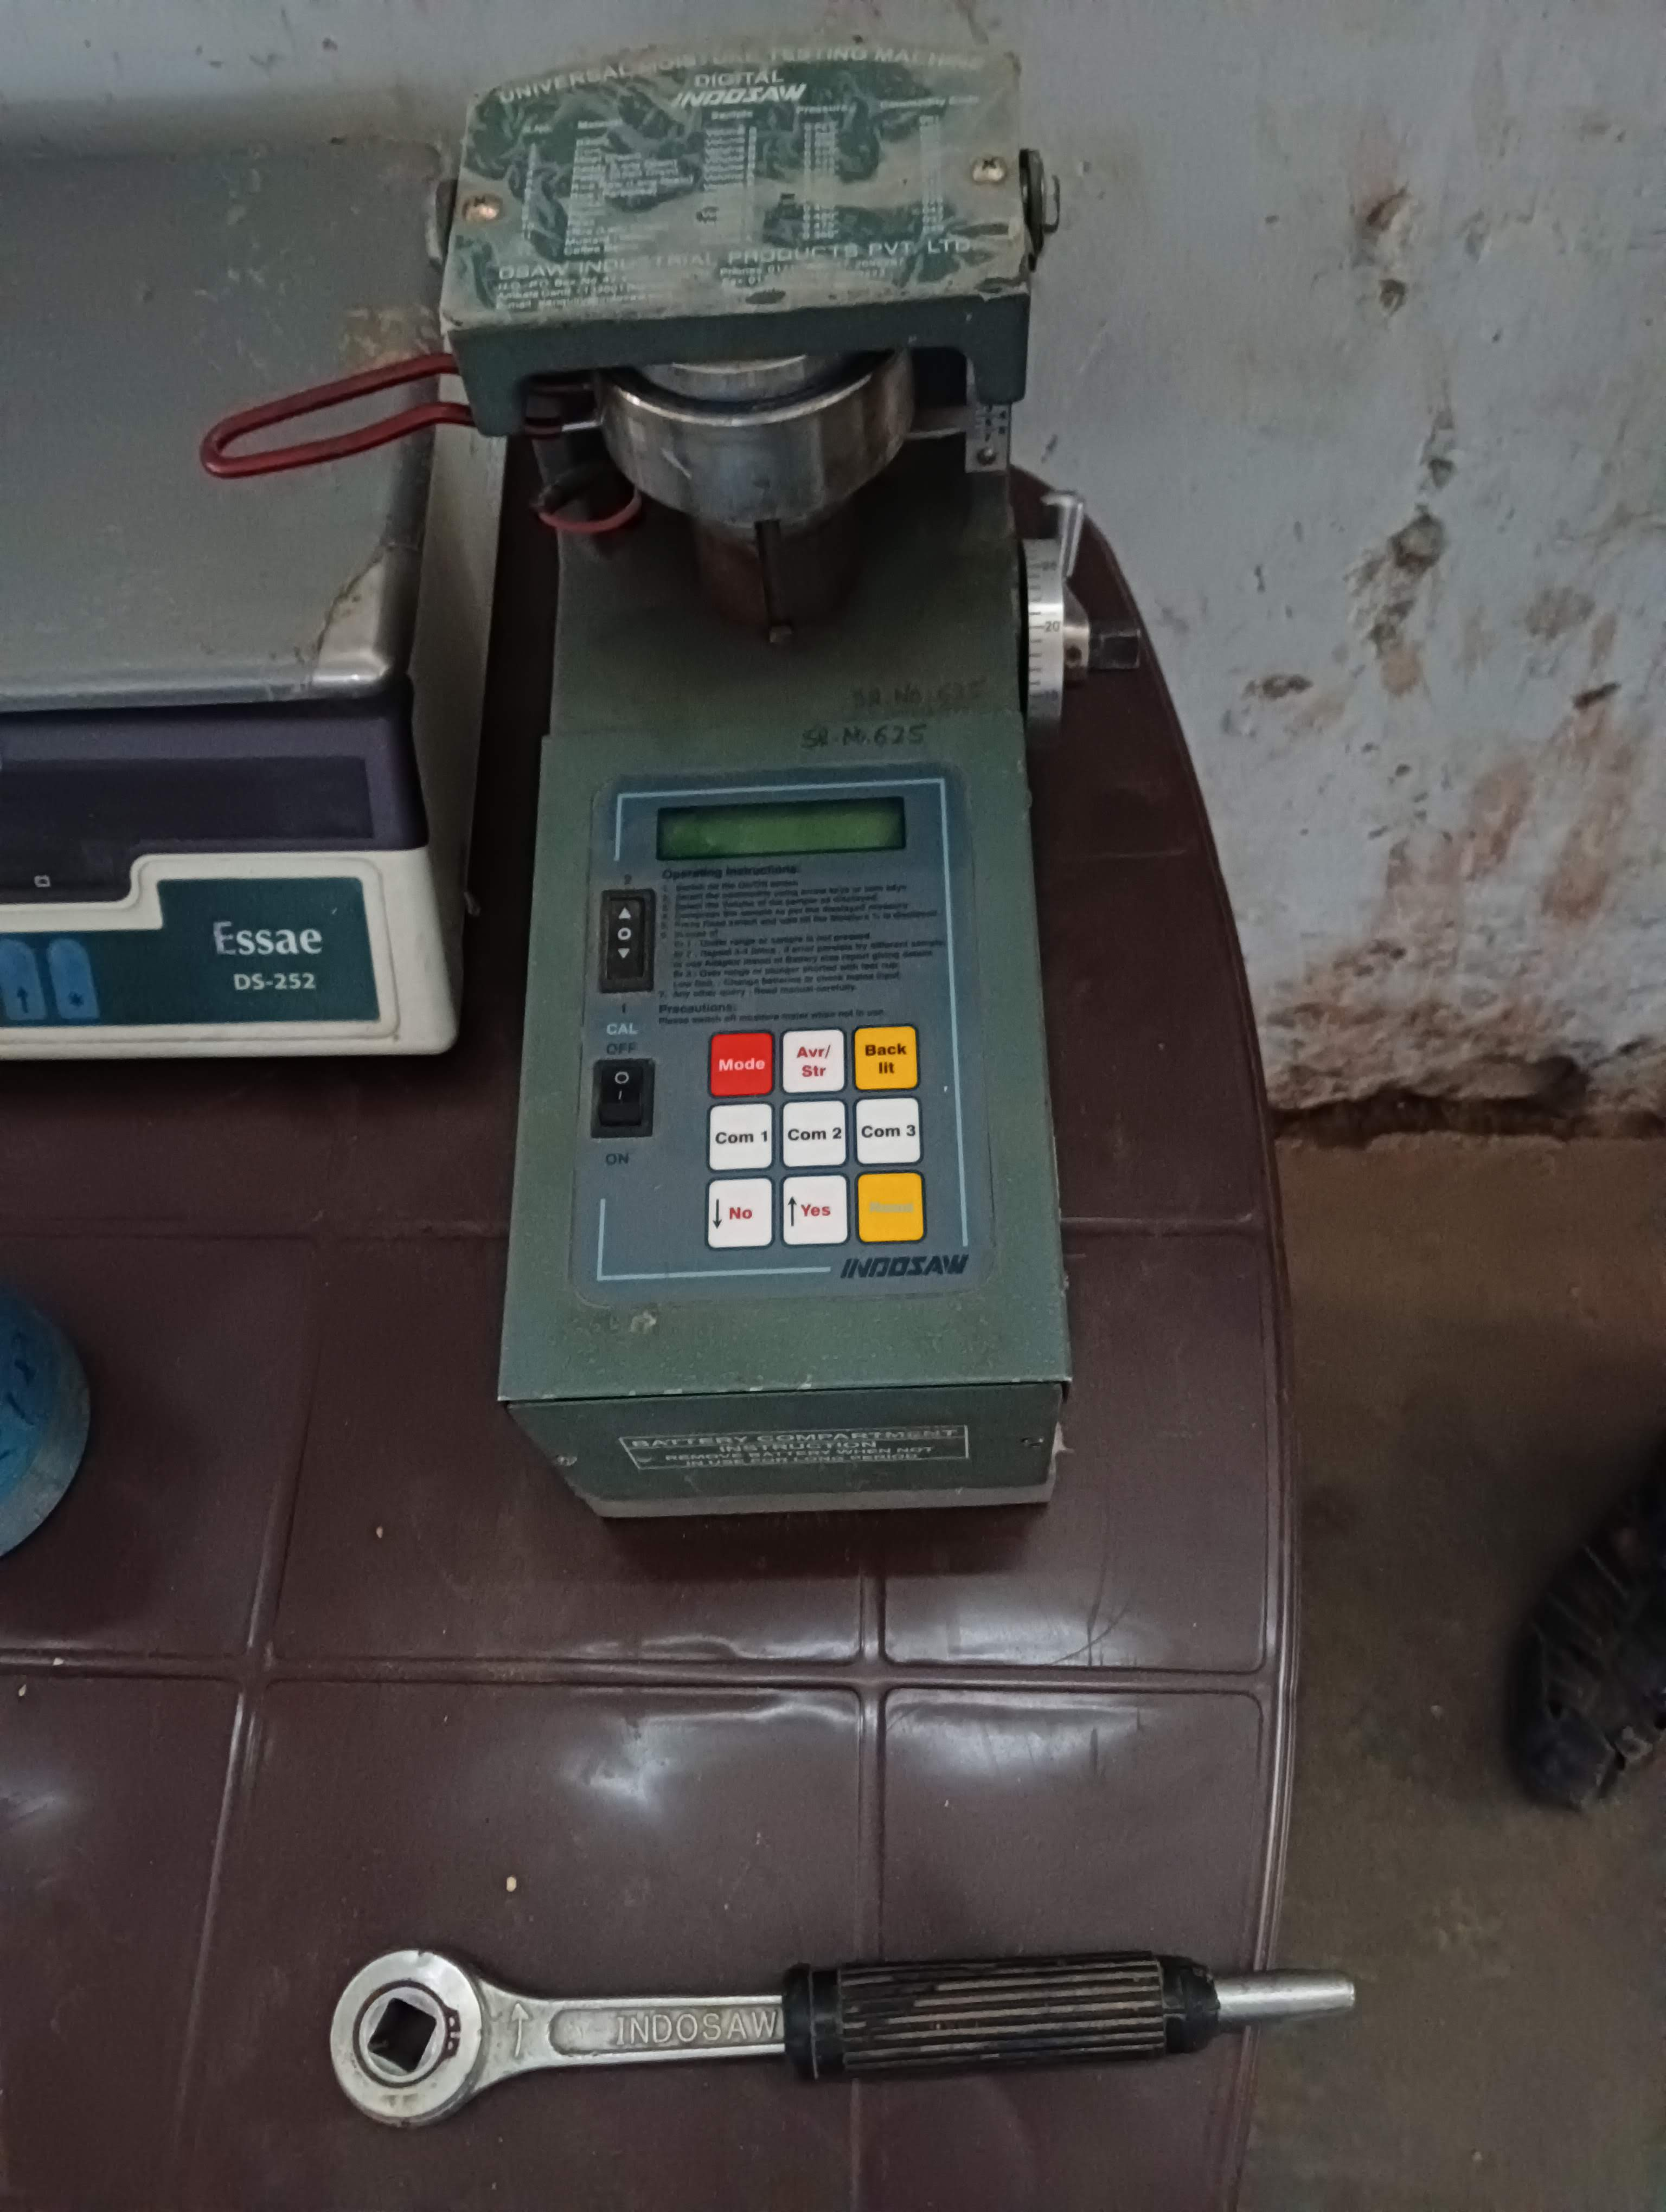
\includegraphics[width=0.8\textwidth]{moisture measurement in godown.jpg}
        \caption{Moisture content reading.}
        \label{fig:moisture_meter}
    \end{subfigure}
    \hfill
    \begin{subfigure}[b]{0.48\textwidth}
        \centering
        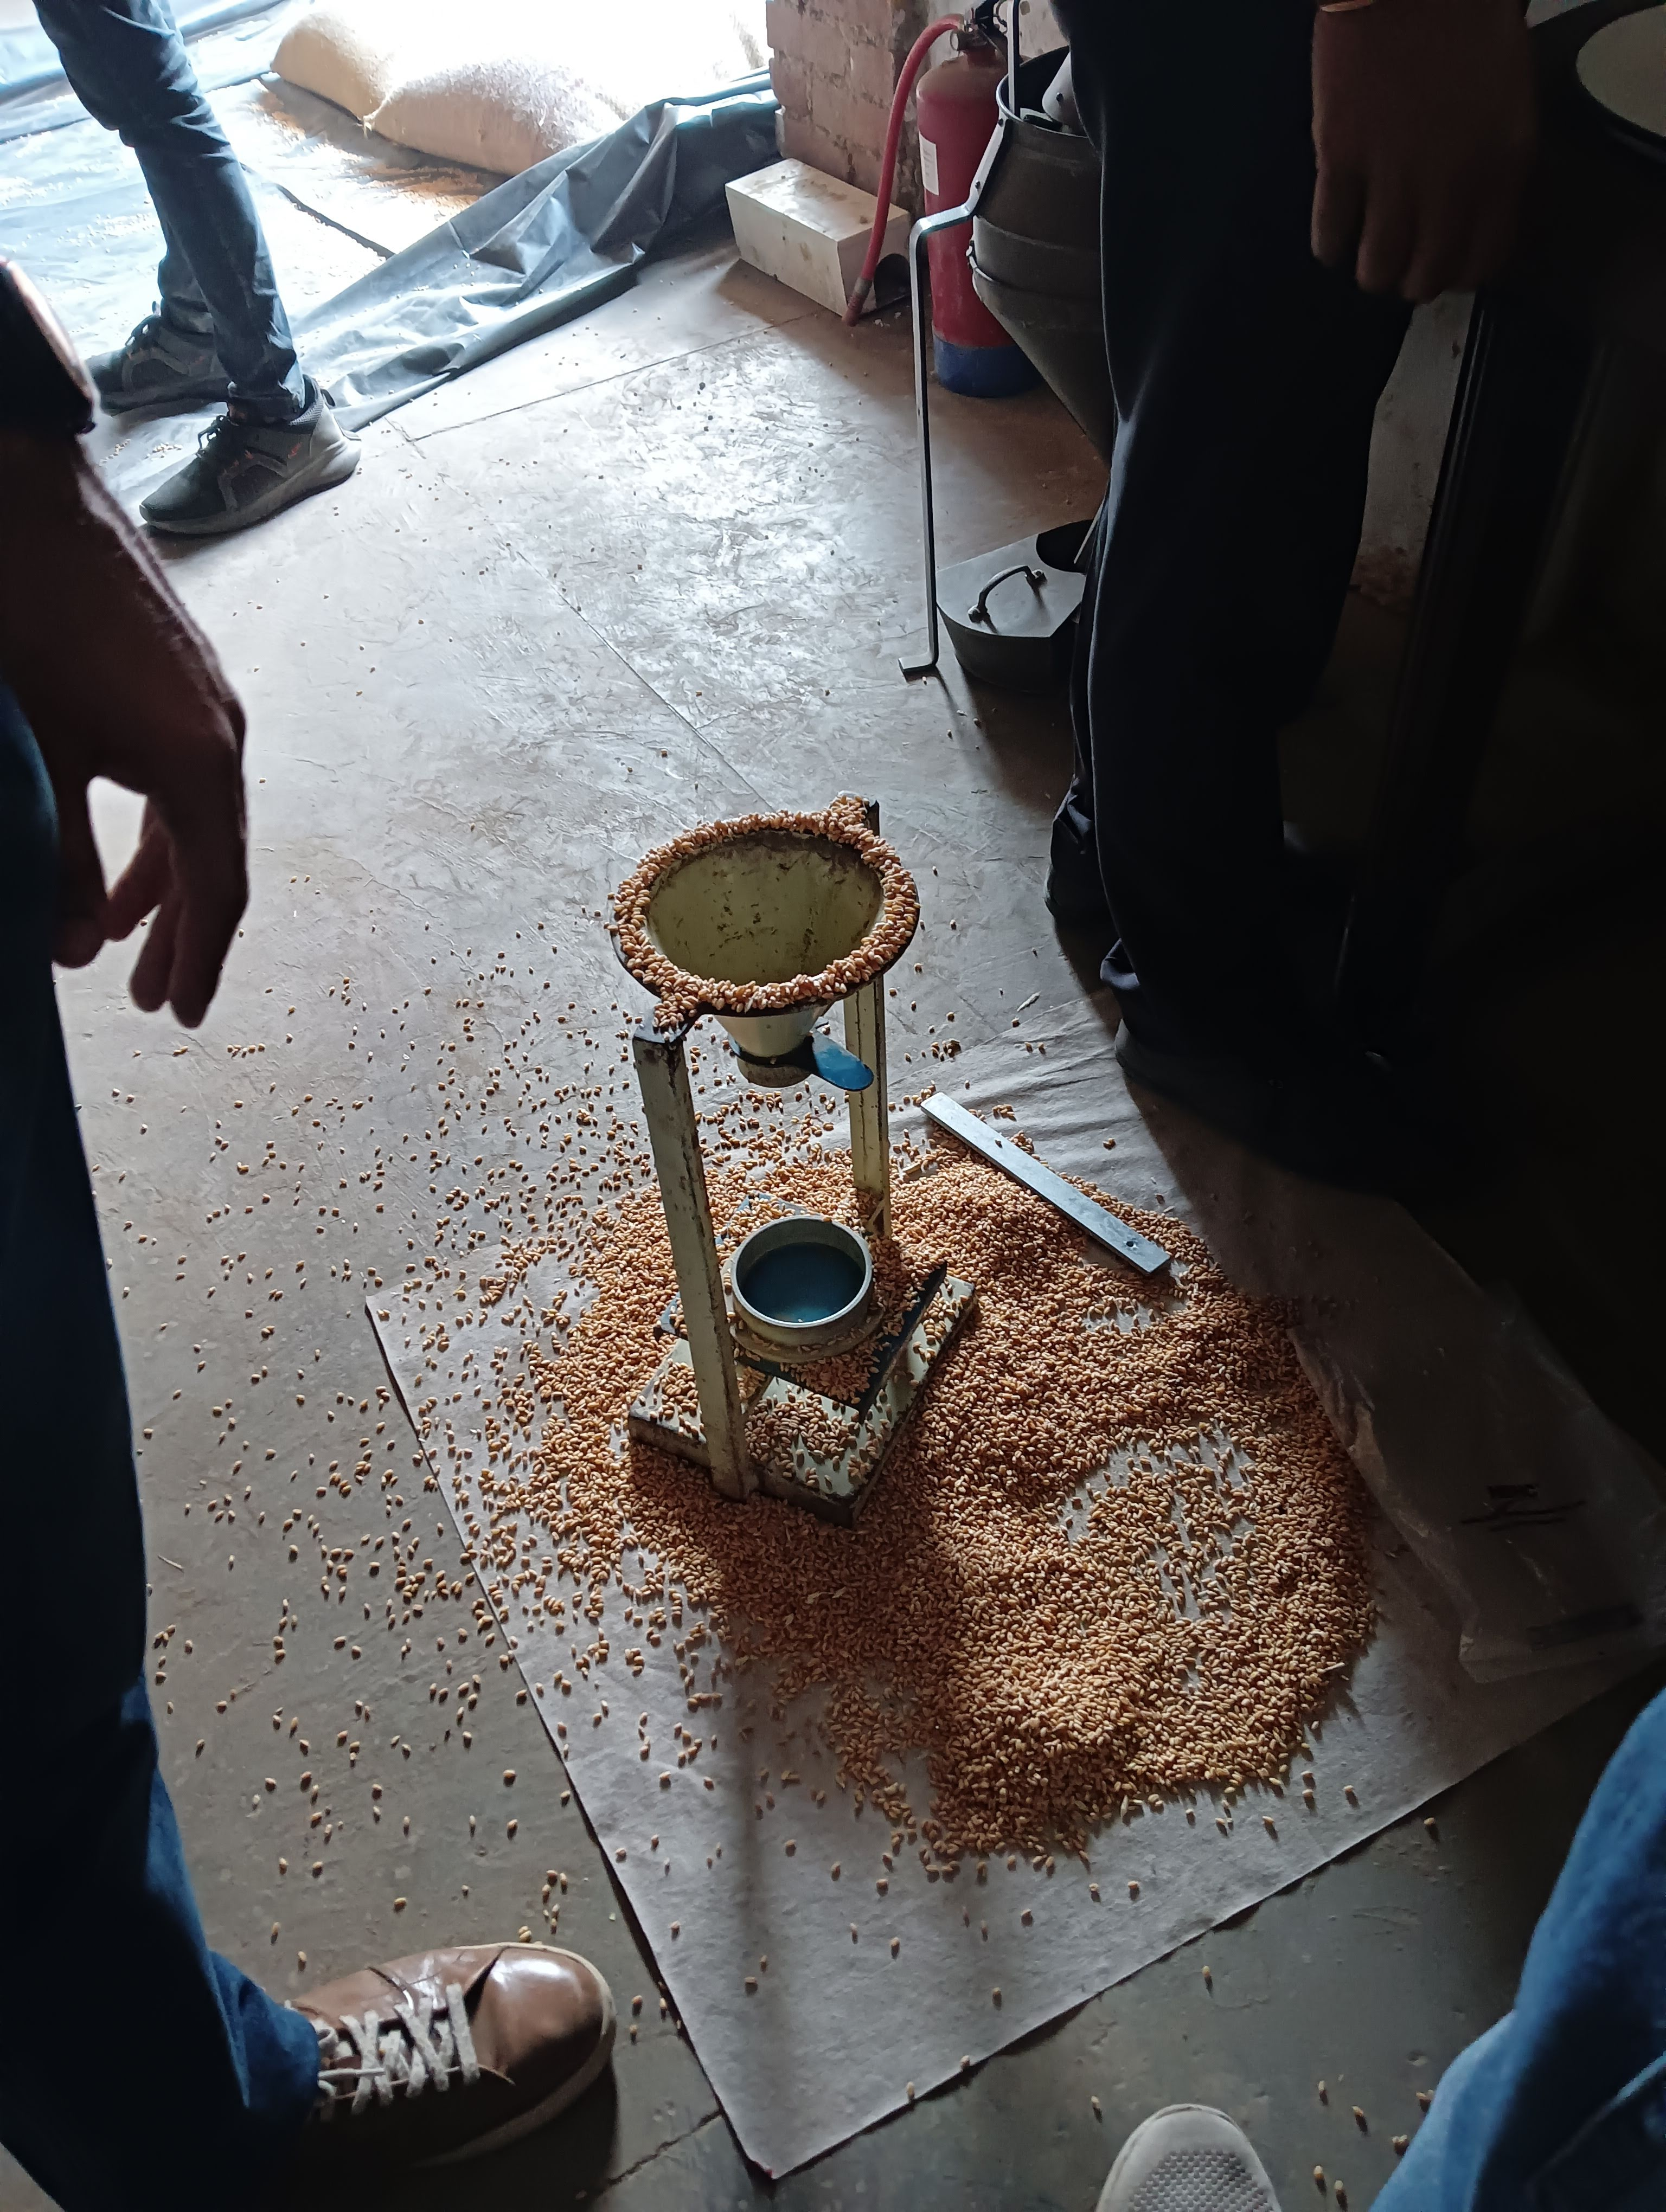
\includegraphics[width=0.8\textwidth]{Hectolitre weight measurement in godown.jpg}
        \caption{Hectolitre weight recording.}
        \label{fig:hectolitre_weight}
    \end{subfigure}
    \caption{Initial checks grains and impurities segregation: (a) moisture measurement and (b) Hectolitre weight for wheat variety verification.}
    \label{fig:periphery_tests}
\end{figure}

\subsection{Threshold Logic and the $W/W\%$ Calculation}

For each category, $W/W\%$ is calculated and compared with standard procurement thresholds. Acceptance requires impurity and defect percentages to remain below category limits. Pure wheat has no upper cap; a higher proportion indicates better lot quality.

\subsection{Master Sample and Redundancy}

If the periphery result is acceptable, unloading proceeds and a master sample is drawn from inner \textit{boris}. The full test is repeated to verify that inner-lot quality matches the outer-lot sample and to reduce adulteration risk.

\begin{figure}[H]
    \centering
    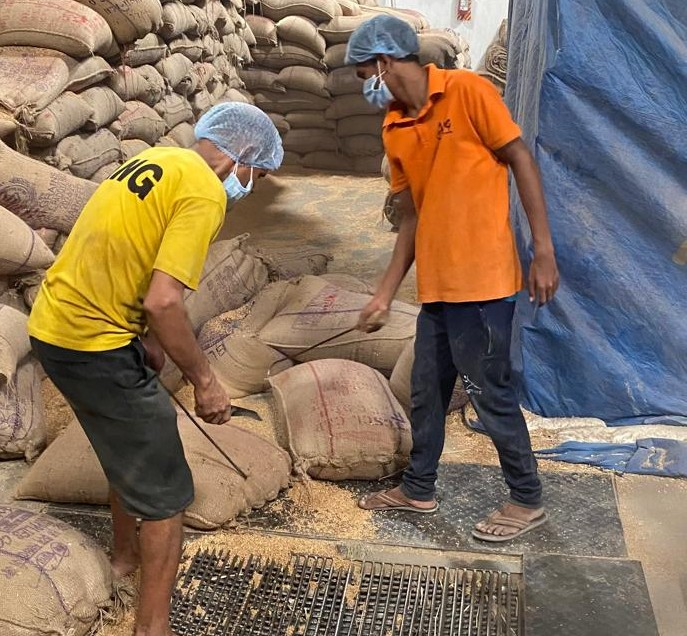
\includegraphics[width=0.45\textwidth]{factory sample collection from bori.jpeg}
    \caption{Master sample collection from \textit{boris} at godown.}
    \label{fig:sample_collection}
\end{figure}

%----------------------------------------------------------------------------------------
\section{Synthesis of Design Constraints}
%----------------------------------------------------------------------------------------

Four design constraints emerged from fieldwork:

\textbf{Latency:} Sixty minutes per sample is a physical consequence of one person sorting 2,800 grain entities by hand. The target cycle time for Drishti was set at under five minutes. Anything slower than ten minutes would provide insufficient operational benefit to justify adoption.

\textbf{Expertise concentration:} Experienced and inexperienced assessors are not interchangeable in practice. Agreement was high on major categories but varied significantly on borderline specimens, such as a kernel that reads as either \textit{Broken} or \textit{Sharbati} depending on assessor experience. A system that classifies independently of the operator removes this source of variance.

\textbf{Environmental consistency:} Dust, variable lighting, and shift-length fatigue progressively degrade classification reliability. Late-shift assessments showed more conservative borderline calls and slower sorting speeds than early-shift assessments. An automated system does not accumulate fatigue.

\textbf{Adulteration detection:} Quality managers described a specific practice: blending lower-grade grain into premium-variety lots, concentrated toward the inner \textit{boris} furthest from the periphery sample draw. The two-stage sampling protocol is specifically designed to catch this. An automated system must match the sensitivity of the most experienced assessors to avoid enabling rather than preventing quality fraud.
 
%% Chapter 3 --- Literature Review and State of the Art

\chapter{Literature Review and State of the Art}\doublespacing
\label{Chapter3}
\lhead{Chapter III. \emph{Literature Review and State of the Art}}

%----------------------------------------------------------------------------------------
\section{Computer Vision in Agriculture: A Trajectory}
%----------------------------------------------------------------------------------------

Before describing what this research does, it helps to be clear about what already exists and why it is not sufficient.

The application of computer vision to agricultural grain assessment has a reasonably long history, and the results are, in aggregate, encouraging but conditional. Early systems relied on handcrafted feature descriptors---shape measurements, texture statistics derived from grey-level co-occurrence matrices, colour histogram profiles---fed into classical classifiers such as SVM or k-NN. The survey by \cite{Lingwal2021} provides a systematic account of this era. The recurring finding is that these approaches work well in controlled settings and considerably less well when the conditions of image acquisition vary. Lighting angle, grain orientation, and regional morphological differences between wheat varieties all degrade performance in ways that handcrafted features have limited ability to compensate for.

The introduction of convolutional neural networks changed the picture substantially. By learning discriminative visual features from labelled data rather than from manually specified rules, CNN-based systems showed robustly improved variety-level classification performance. Studies by \cite{Laabassi2021} and \cite{Yasar2024} demonstrate successful discrimination between \textit{Sharbati}, \textit{Durum}, and \textit{Lokwan} varieties under reasonably realistic conditions. The qualitative shift in capability is real. What is less often acknowledged is the distributional assumption embedded in most reported evaluations: the test samples are sparse, carefully arranged, and photographed under controlled illumination. That is not the operating environment this research needed to address.

%----------------------------------------------------------------------------------------
\section{The Paradox of YOLO in High-Density Environments}
%----------------------------------------------------------------------------------------

YOLO-family detectors have become near-ubiquitous in real-time vision applications, and their deployment profile---single forward pass, fast inference, modest computational footprint---makes them attractive for edge deployment \cite{YOLOReview2024}. For many agricultural tasks, they perform well. Dense wheat-bed assessment is an exception worth examining carefully.

A 100-gram wheat sample placed on a flat tray presents roughly 2,800 grain entities in close proximity. Under these conditions, two effects become dominant. First, heavy mutual overlap produces prediction conflicts that non-maximum suppression handles poorly, generating undercounts and merged detections \cite{YOLODense2025}. Second, the anchor and grid assumptions on which YOLO architectures are built are stressed when target instances are very small relative to the local receptive field, as is the case with a 3--5 mm wheat kernel in a wide-field overhead image.

Comparable failure modes appear in other dense-entity domains: crowd counting, histological cell segmentation, and agricultural spike density estimation. The pattern is consistent enough that it should be taken as a structural property of the problem rather than a failure mode that can be patched by choosing a better model. Even architectures with stronger localization mechanisms, such as Mask R-CNN variants examined by \cite{Xu2023}, require substantial task-specific adaptation under dense occlusion. The implication, which took some time to fully accept, is that pushing on the model side alone is unlikely to solve the problem. The physical presentation of the sample needs to change first.

%----------------------------------------------------------------------------------------
\section{The Occlusion Problem and the Single-View Assumption}
%----------------------------------------------------------------------------------------

There is an assumption buried in the design of most automated grain quality studies that deserves explicit examination: that a single overhead image of a grain sample contains sufficient information for classification. For broad morphological assessments---separating wheat from chaff, or whole kernels from broken ones---this is probably true. For ITC's twelve-category protocol, it is not.

Several defect signatures are geometrically orientation-sensitive. The diagnostic features of early-stage \textit{Infested} grain---characteristic entry points on the kernel surface---are not visible from above if the kernel happens to lie with that surface downward. The darkening that marks \textit{Black Tip} and \textit{Kernel Burnt} specimens is similarly distributed in ways that depend on how the grain has settled. \cite{ShenUnsound2023} reported systematic under-detection of ventral-side defects in single-image acquisition settings, which is precisely the failure mode most damaging for quality assessment: the system confidently misclassifies because it is literally not seeing the relevant evidence.

Multispectral and hyperspectral imaging approaches \cite{LiWheat2024, ElMasry2019} offer improved spectral contrast for certain defect types, but they do not resolve geometric occlusion. A hyperspectral sensor imaging a wheat grain that is lying on its diagnostic surface still cannot see that surface. The problem is one of physical observability, and improving the sensor does not address it.

%----------------------------------------------------------------------------------------
\section{Hardware-Software Co-Design: Engineering Observability}
%----------------------------------------------------------------------------------------

The concept of hardware-software co-design \cite{Keutzer2000} was developed in the context of embedded processor architecture, but the underlying logic transfers to this problem directly: rather than asking the software to compensate for the limitations of the physical setup, design the physical setup to present the software with a well-posed problem.

Applied to dense grain assessment, this means accepting that occlusion is a physical phenomenon before it is a computational one. If grains can be separated and their orientation varied during image acquisition, the vision model is no longer being asked to infer what it cannot see; it is being presented with isolated, diverse views of each specimen and asked to classify from good evidence. The computational task becomes substantially easier, and the performance of a well-trained classifier becomes predictably better.

This logic is not novel in industrial inspection. Automated optical inspection systems in electronics manufacturing have long been co-designed so that mechanical handling---conveyors, positioning fixtures, rotation stages---provides the visual access that the imaging system requires \cite{Newman1995}. The contribution of this research is to adapt and develop that logic for agricultural grain assessment, a context that introduces additional complications: highly variable grain morphology, a bulk sample (rather than individually fixtured components), operational environments with dust and time pressure, and the need for the mechanical handling system to be fast, gentle, and reliable across thousands of cycles.

%----------------------------------------------------------------------------------------
\section{Summary}
%----------------------------------------------------------------------------------------

Reading through this body of work clarified the research problem at a level of precision that the fieldwork alone could not provide. Deep learning models are demonstrably capable of grain classification when the imaging conditions are favourable. The problem is that industrial procurement conditions are not favourable, and the gap between the laboratory settings of published evaluations and the warehouse floor is wide enough to be decisive. The single-view assumption and the density-related failure modes of current detectors both point toward the same architectural intervention: design the hardware to improve observability before asking the software to classify. Chapter~\ref{Chapter4} describes how that principle was translated into an actual design process.

% Chapter 4 --- Design Methodology and Iterative Prototyping

\chapter{Design Methodology and Iterative Prototyping}\doublespacing
\label{Chapter4}
\lhead{Chapter III. \emph{Design Methodology and Iterative Prototyping}}

%----------------------------------------------------------------------------------------
\section{Preliminary Visual Analysis and Colour Theory}
%----------------------------------------------------------------------------------------

A structured visual analysis was conducted across all twelve target categories using physical grain specimens from procurement sites. The working question was: \textit{which visual cues do experienced assessors use when making a category call, and can controlled illumination make those cues measurable by a camera?}

Early experiments used coloured chart-paper backgrounds at varied light angles. Warm amber tones improved contrast between \textit{Lokwan} and \textit{Kernel Burnt}; cooler backgrounds improved boundary definition for segmentation. No single background setting performed consistently across all twelve categories and wheat varieties.

This led to the first key design decision: replace static backgrounds with a programmable active substrate. An LCD panel beneath a transparent imaging surface \cite{ElMasry2019} allows the background colour to be set per variety. A dual-illumination architecture combining a top-mounted RGB ring light with a variable LCD background became the basis for subsequent prototypes.

\begin{figure}[H]
    \centering
    \begin{subfigure}[b]{0.30\textwidth}
        \centering
        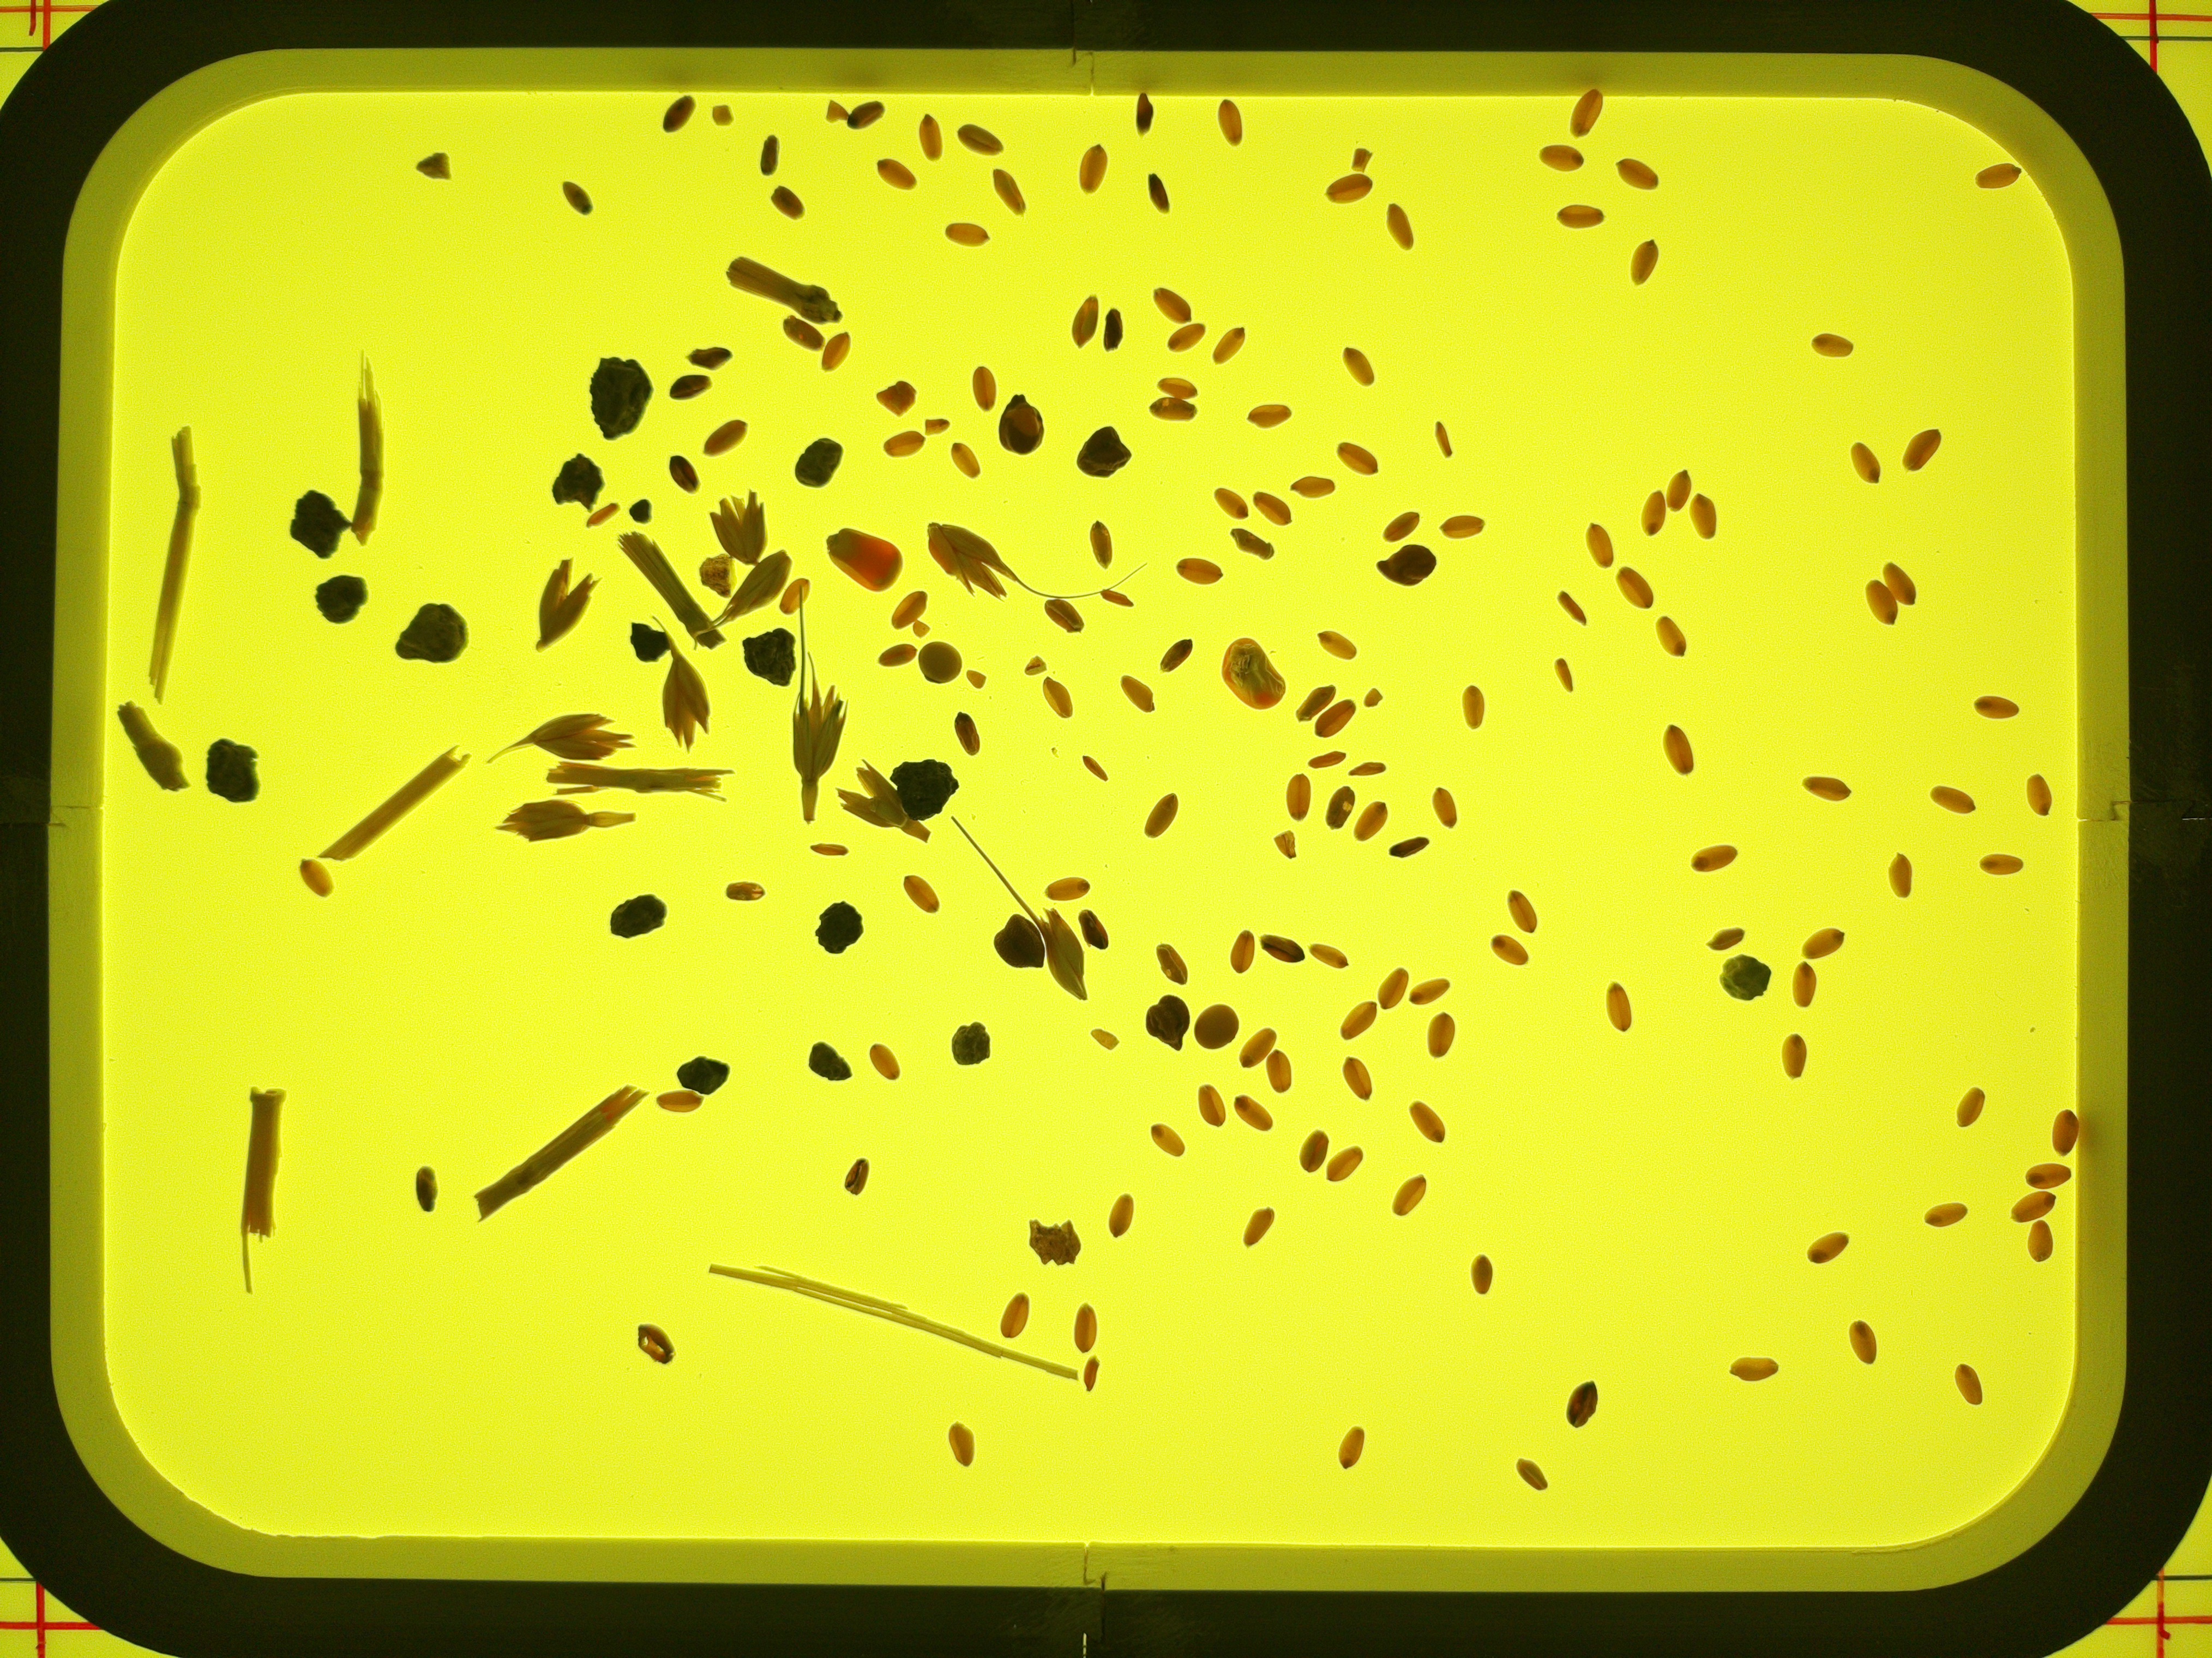
\includegraphics[width=\textwidth]{BY - yellow from bottom only - for segmentation.jpg}
        \caption{BY}
        \label{fig:colour_by}
    \end{subfigure}
    \hfill
    \begin{subfigure}[b]{0.30\textwidth}
        \centering
        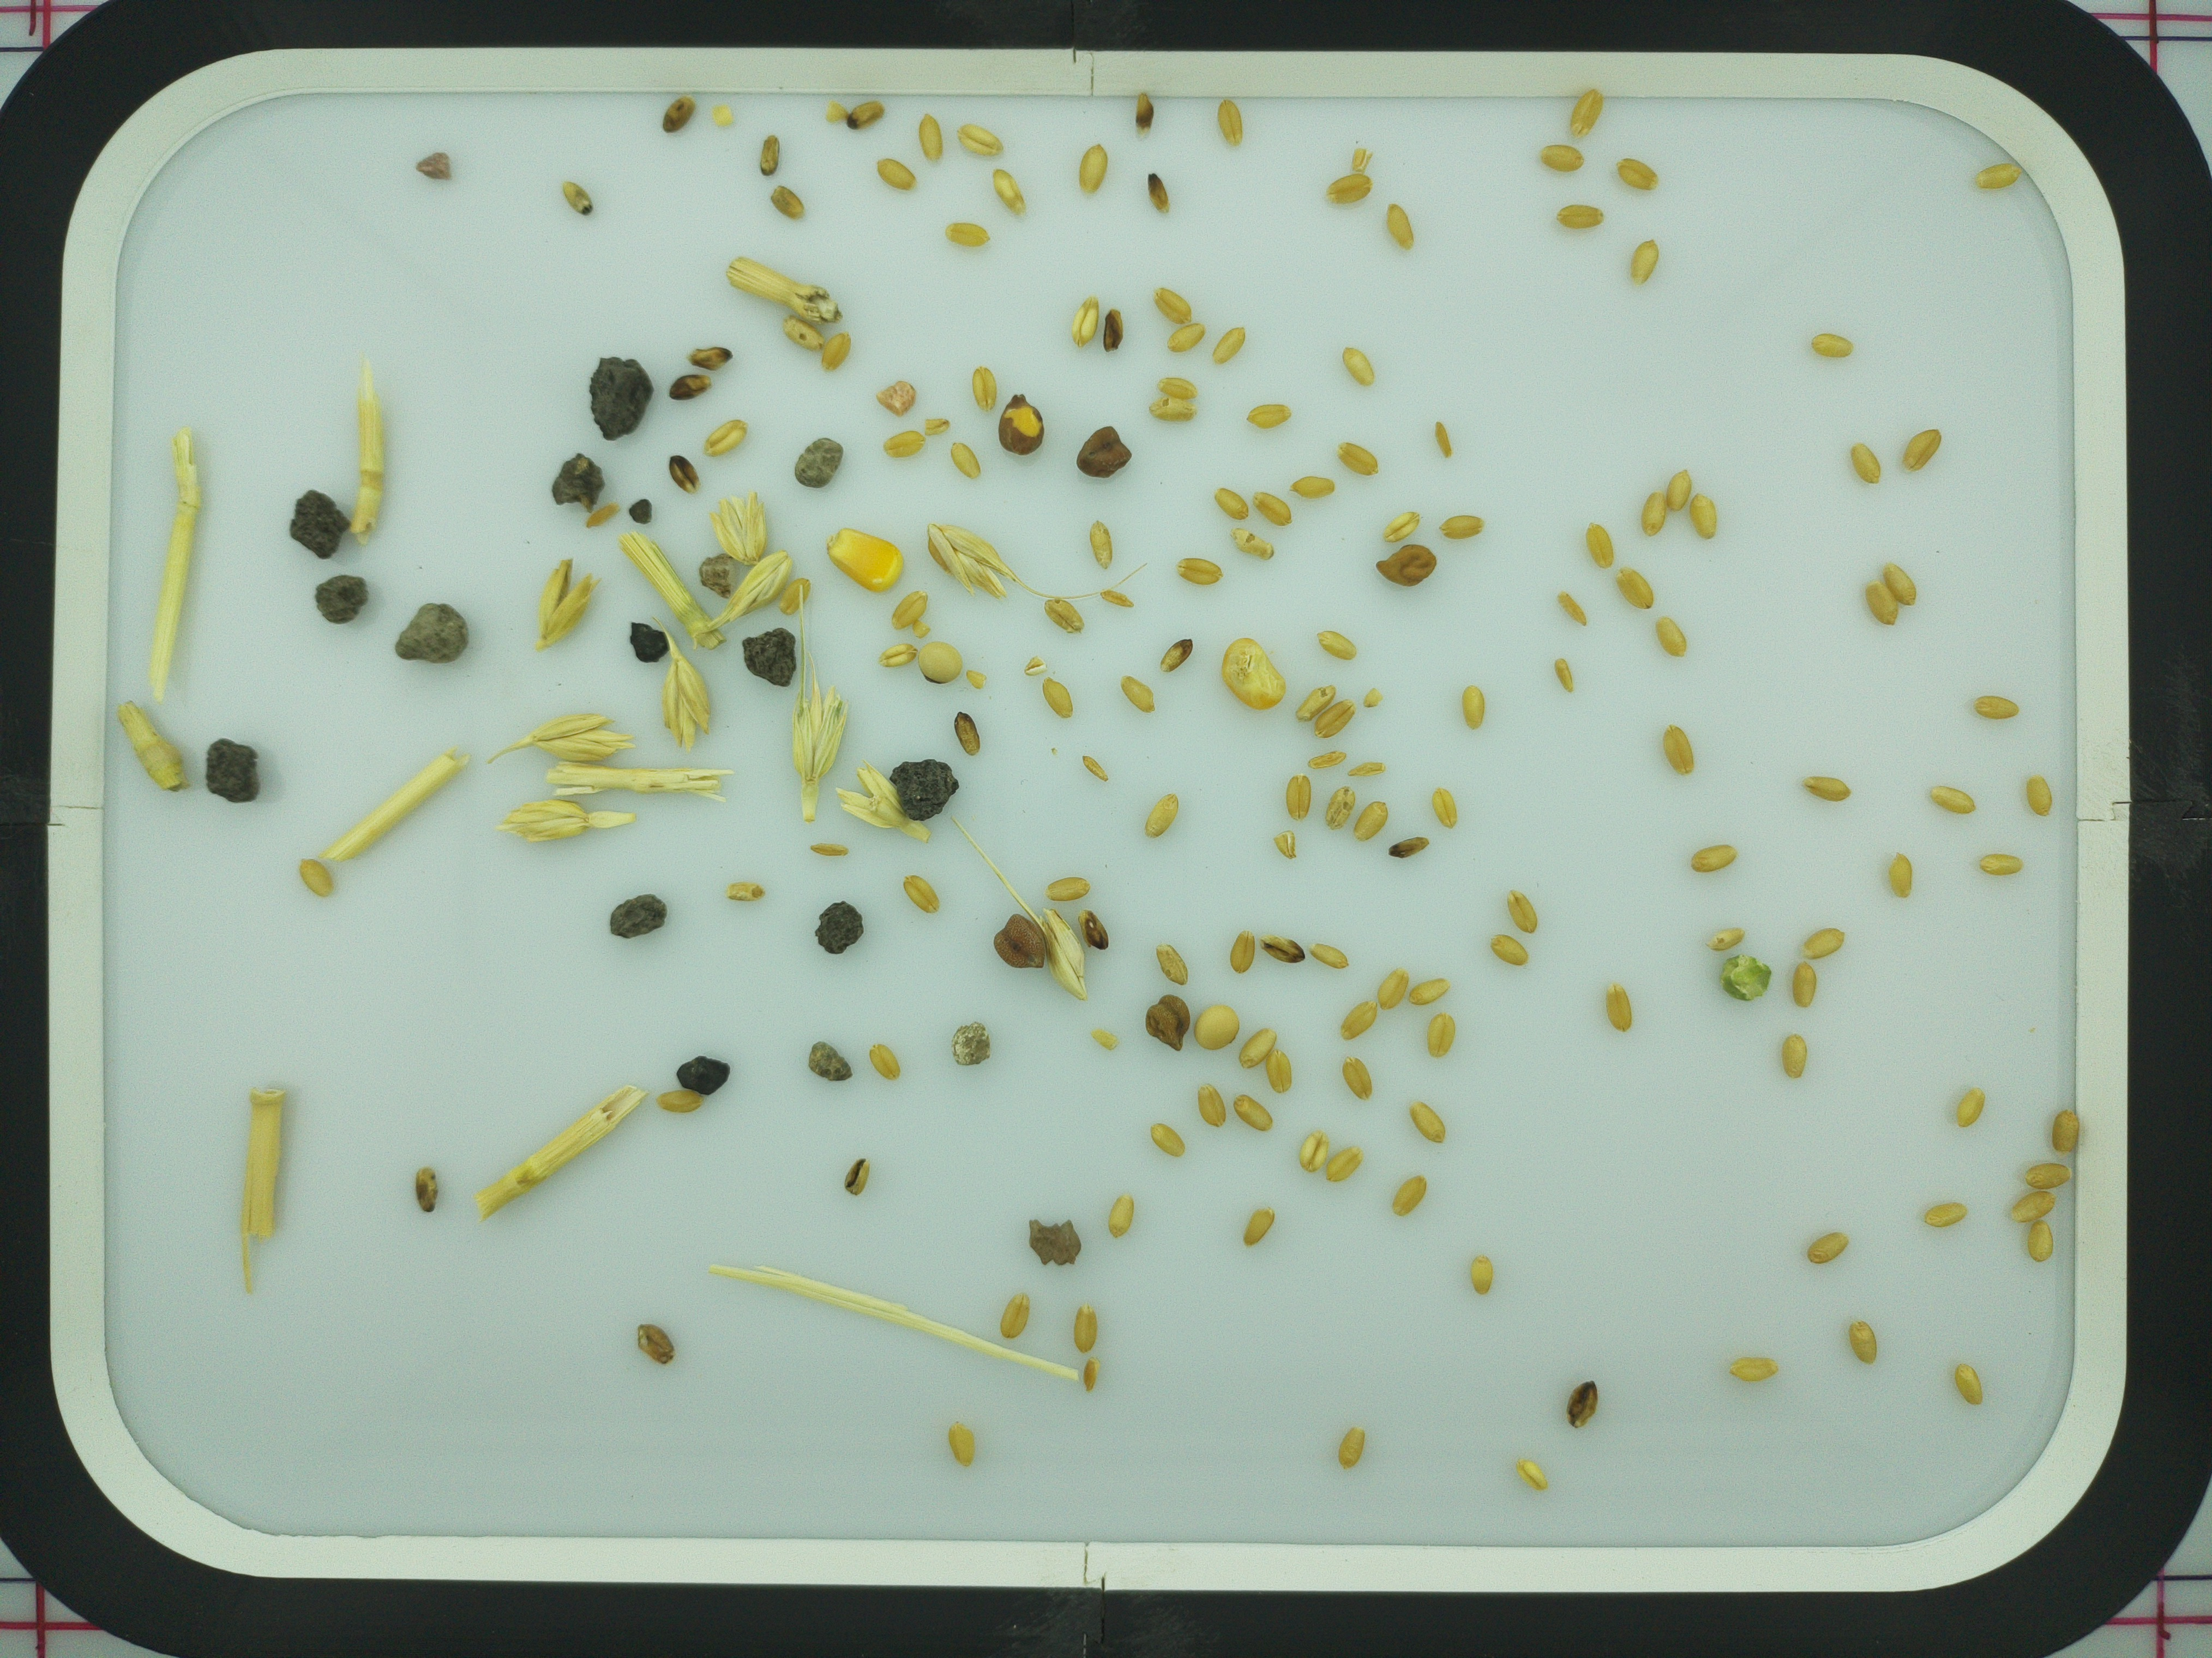
\includegraphics[width=\textwidth]{WB - white from top only - for classiication.jpg}
        \caption{WB}
        \label{fig:colour_wb}
    \end{subfigure}
    \hfill
    \begin{subfigure}[b]{0.30\textwidth}
        \centering
        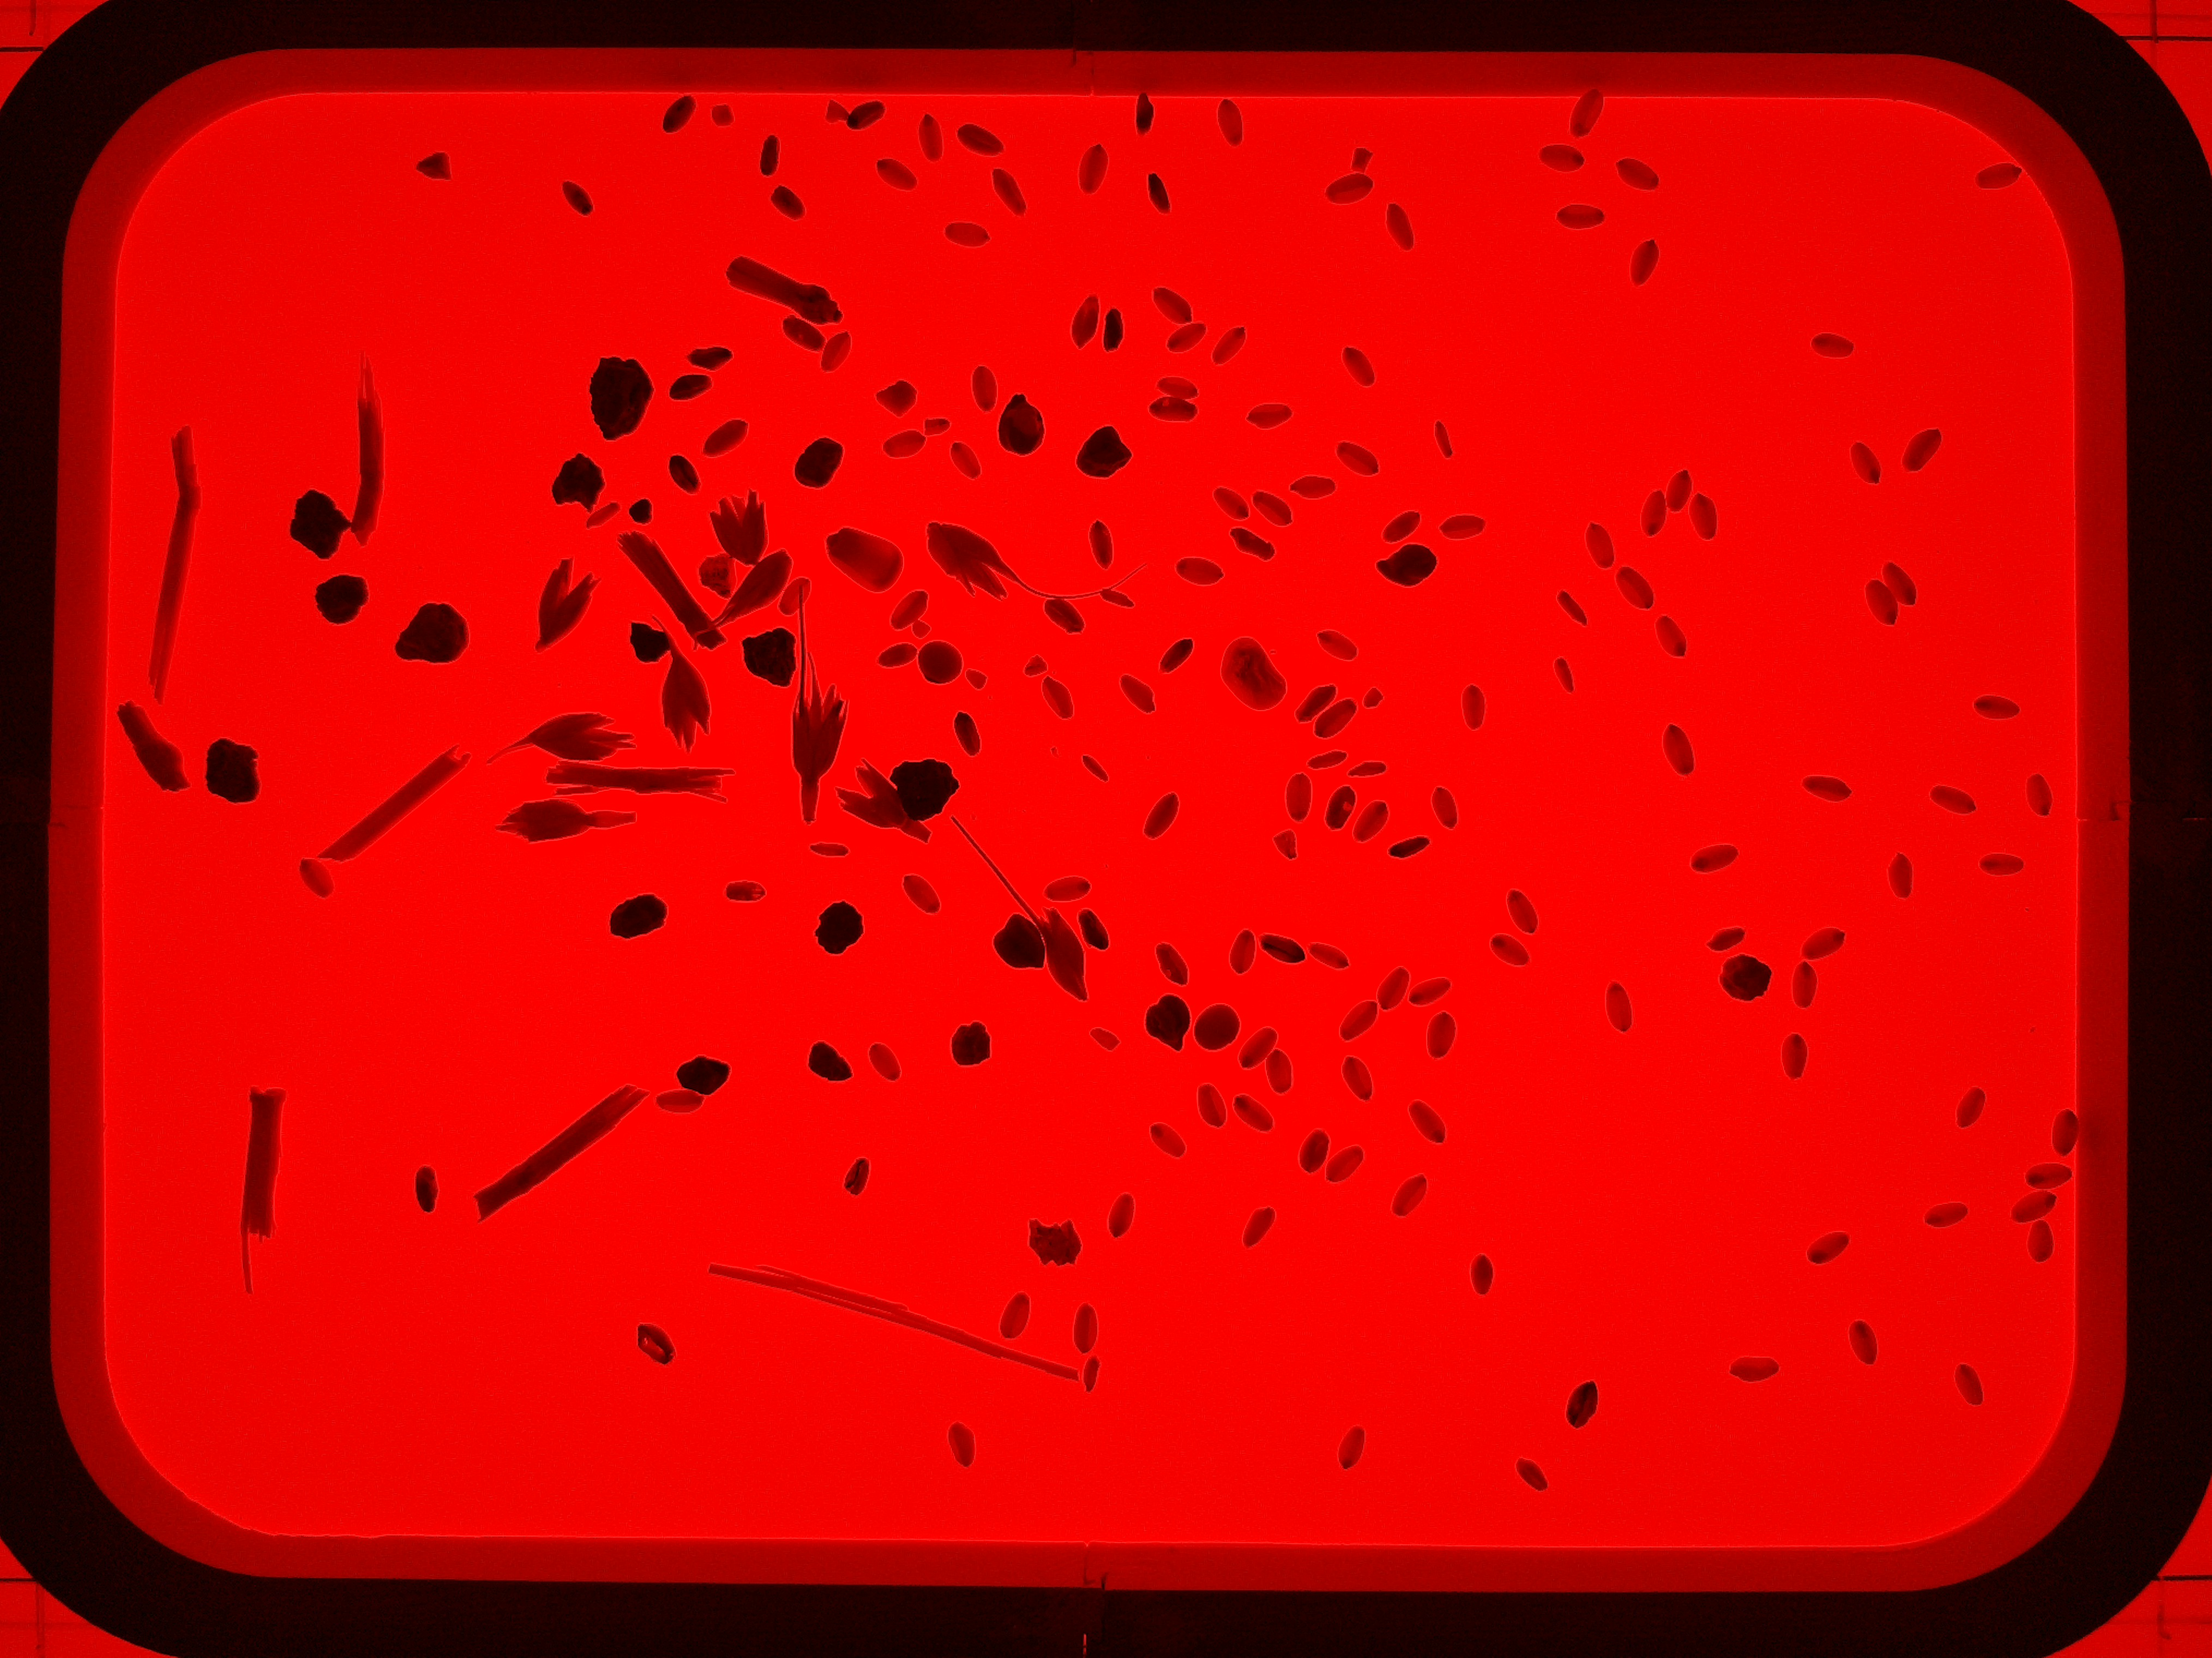
\includegraphics[width=\textwidth]{BR - Red from bottom only - for multispectral classification.jpg}
        \caption{BR}
        \label{fig:colour_br}
    \end{subfigure}
    \caption{Final illumination configurations: (a)~BY yellow backlight for grain boundary segmentation, (b)~WB white top-light for general classification, and (c)~BR red backlight for multispectral defect classification.}
    \label{fig:figure4_1}
\end{figure}

%----------------------------------------------------------------------------------------
\section{Prototype I: Low-Fidelity Proof of Concept}
%----------------------------------------------------------------------------------------

Prototype I used a 3D-printed enclosure, a small LCD panel as the active background, WS2812B top illumination, and a Raspberry Pi 5 for control and capture. The objective was to verify the dual-illumination hypothesis in practice. The combined top-light and programmable backlight improved visual separation between categories that static backgrounds could not distinguish. Early-stage \textit{Infested} specimens became more distinguishable under certain background settings. However, the small enclosure handled only a fraction of a 100-gram sample. Scaling to operational volume required a separate design effort.

\begin{figure}[H]
    \centering
    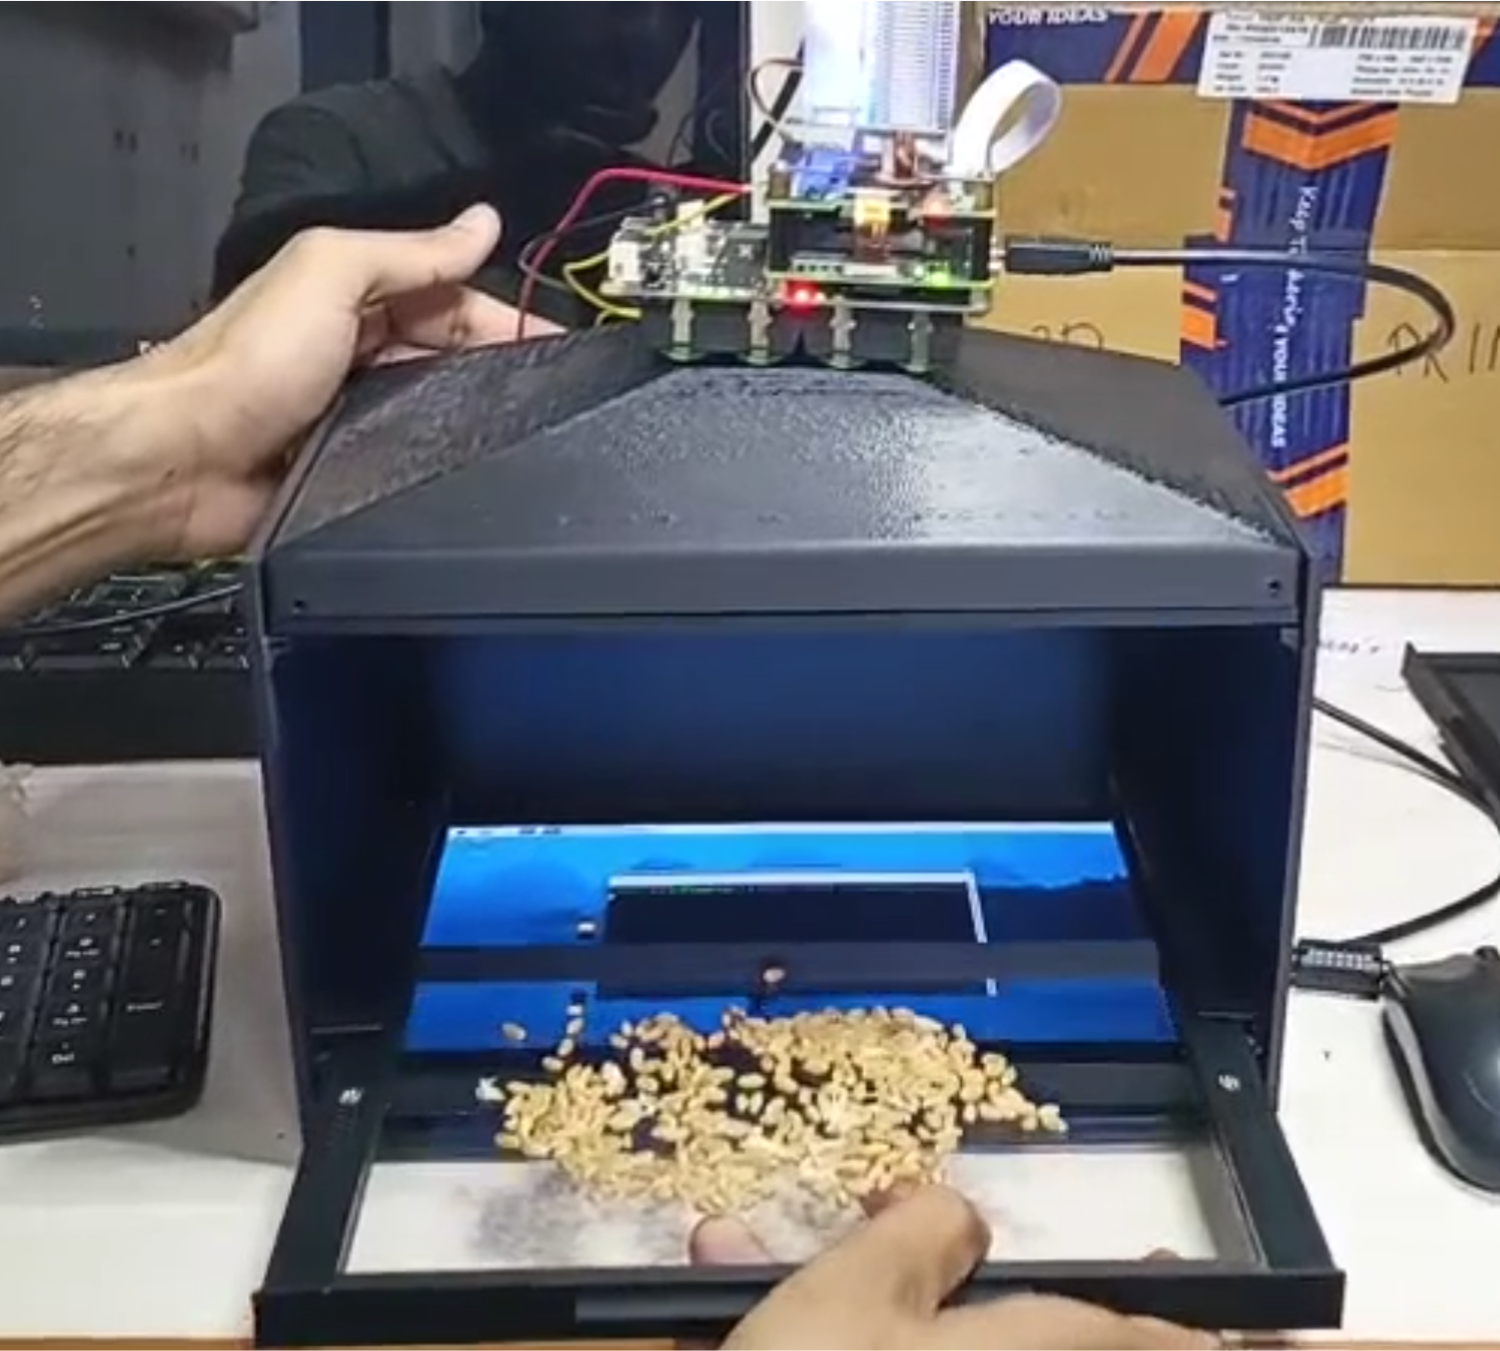
\includegraphics[width=0.65\textwidth]{3d printed prototype.png}
    \caption{Prototype~I: low-fidelity 3D-printed enclosure validating the dual-illumination hypothesis.}
    \label{fig:figure4_2}
\end{figure}

%----------------------------------------------------------------------------------------
\section{Prototype II: Scaling to Industrial Volume and the Density Problem}
%----------------------------------------------------------------------------------------

Prototype II replaced the 3D-printed chassis with aluminium extrusion for durability and dust tolerance. The imaging surface was enlarged to accommodate a full 100-gram sample. Under full sample loading, a 100-gram wheat sample does not spread into a monolayer. At approximately 2,800 entities on a flat surface, grains stack against each other. Many specimens are entirely hidden from the overhead camera at any given moment. Inference on Prototype II images produced undercounting, merged detections, and poor classification confidence on occluded specimens. The constraint was in the imaging geometry, not the algorithm.

\begin{figure}[H]
    \centering
    \begin{subfigure}[b]{0.48\textwidth}
        \centering
        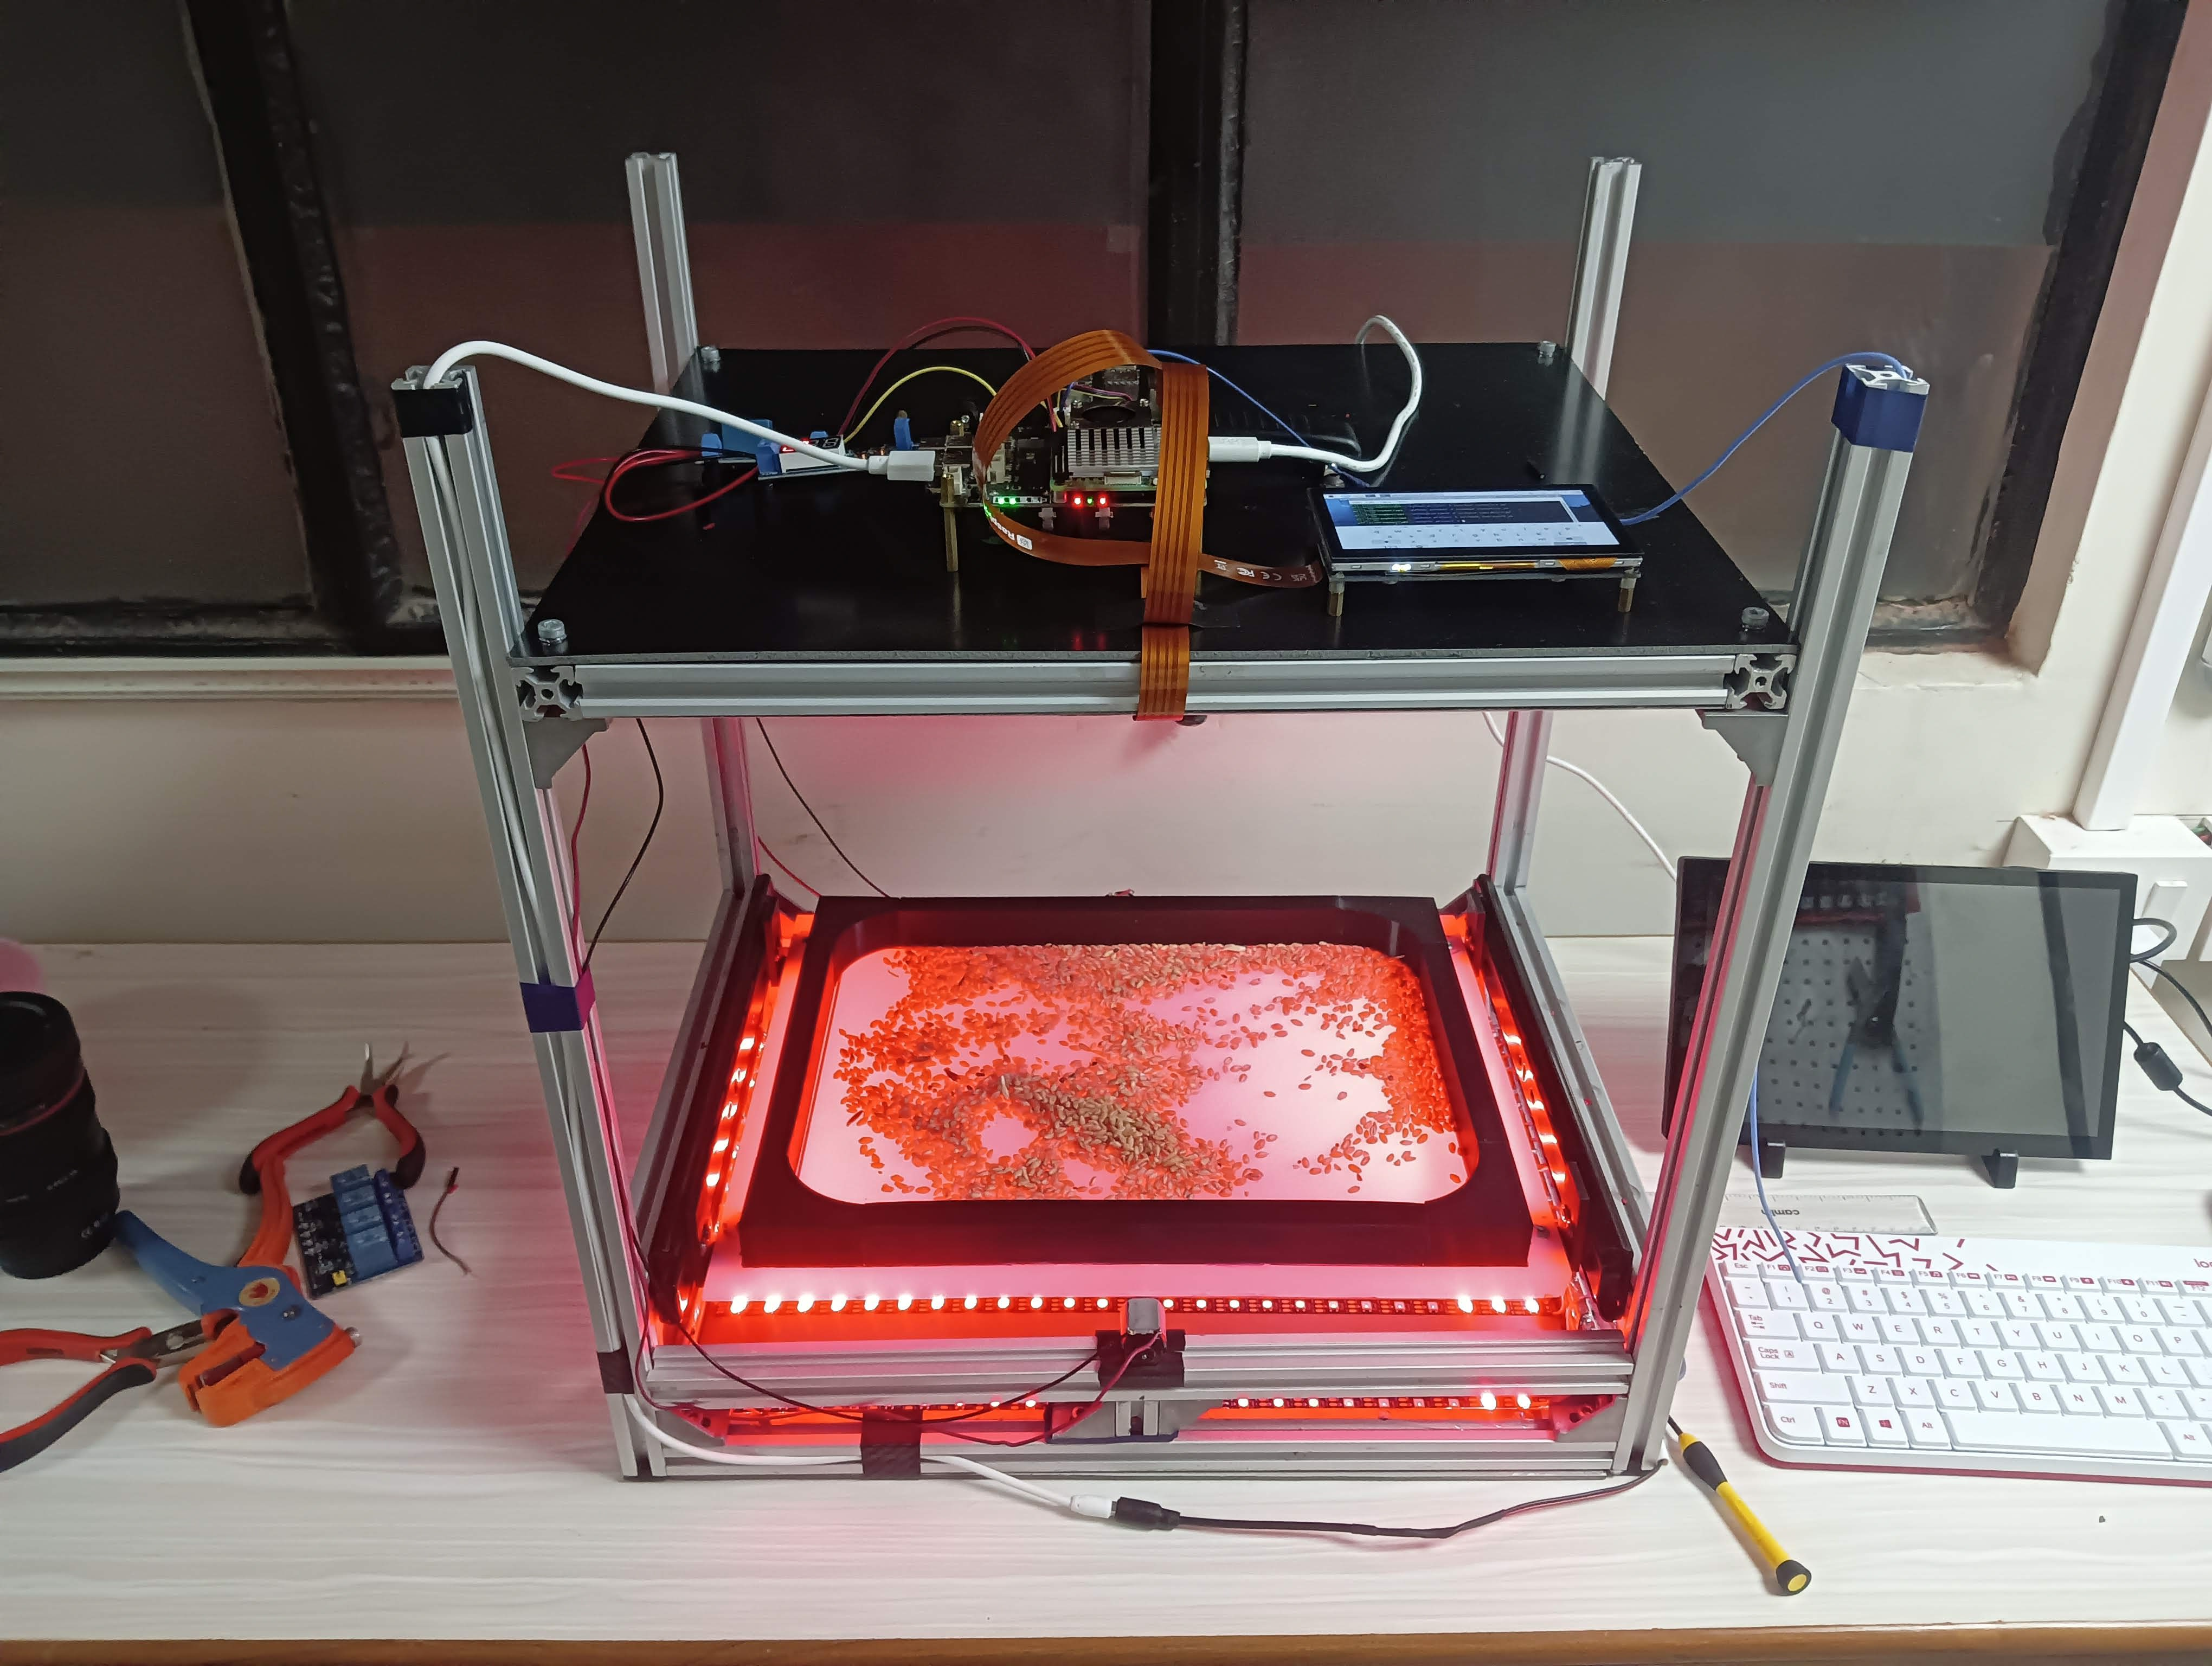
\includegraphics[width=\textwidth]{aluminium prototype.jpg}
        \caption{Aluminium extrusion chassis of Prototype~II.}
        \label{fig:aluminium_chassis}
    \end{subfigure}
    \hfill
    \begin{subfigure}[b]{0.48\textwidth}
        \centering
        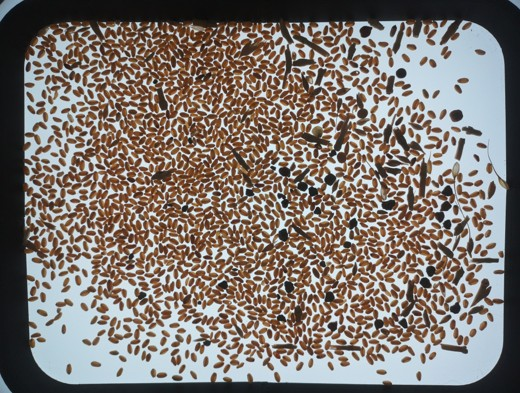
\includegraphics[width=\textwidth]{aluminium prototype sample image.jpg}
        \caption{100-gram sample exhibiting high-density clumping.}
        \label{fig:aluminium_sample}
    \end{subfigure}
    \caption{Prototype~II at industrial scale, showing the high-density occlusion problem that redirected the design brief.}
    \label{fig:figure4_3}
\end{figure}

%----------------------------------------------------------------------------------------
\section{The Hardware-Software Co-Design Pivot}
%----------------------------------------------------------------------------------------

After Prototype II, the design question shifted from ``how do we detect occluded grains?'' to ``how do we ensure grains are not occluded during capture?''

This reframing follows the hardware-software co-design principle \cite{Keutzer2000}: rather than asking software to compensate for physical limitations, the hardware is redesigned so that the computational task becomes tractable. In this case, a mechanical system was required that could disperse a 100-gram sample across a sequence of frames while varying specimen orientations.

The dispersion mechanism had to meet four requirements: repeatability across hundreds of cycles, no damage to grain, compatibility with fine agricultural dust, and a total cycle time under five minutes. Chapter~\ref{Chapter5} describes the mechanical development that met these requirements.
 
% Chapter 5 --- Mechanical Innovation and Granular Dispersion

\chapter{Mechanical Innovation and Granular Dispersion}\doublespacing
\label{Chapter5}
\lhead{Chapter IV. \emph{Mechanical Innovation and Granular Dispersion}}

%----------------------------------------------------------------------------------------
\section{The Necessity of Mechanical Dispersion}
%----------------------------------------------------------------------------------------

The insight that came out of Prototype II was simple to state and took some time to fully absorb: before the system can classify grains, it has to see them. A top-view camera looking down at a dense, three-dimensional pile of 2,800 wheat entities does not have clear sight of most of them. The entities on the exposed surface are imaged; the others are not. Any $W/W\%$ estimate derived from those visible-surface images alone is, in effect, a statistical guess---it might be accurate on average, or it might not, depending on whether the sample has settled in a representative configuration.

For reliable quality assessment, grains need to be presented to the camera progressively: different specimens visible in different frames, different surfaces of each specimen exposed across a capture sequence. This requires two distinct forms of physical motion. \textit{Lateral dispersion} reduces overlap and moves buried grains to the surface. \textit{Rotational excitation} varies grain orientation so that defect signatures on non-top surfaces---the ventral marks of \textit{Infested} grain, the peripheral darkening of \textit{Black Tip}---are captured in at least some frames. Neither optical filtering nor algorithmic improvement can substitute for this; the information has to enter the imaging system in the first place.

The question was how to generate both types of motion reliably, repeatedly, and without damaging the grain in the process.

%----------------------------------------------------------------------------------------
\section{Failure Analysis: Vibratory Agitation}
%----------------------------------------------------------------------------------------

Vibration was the obvious first candidate. It is widely used in grain handling equipment, the implementation is straightforward, and the hardware cost is modest. Several vibration motor configurations were evaluated---low-, medium-, and high-torque units, at different mounting positions and drive frequencies.

The results were discouraging in three specific ways.

The first problem was what might be called \textit{contact impedance}: the transfer of motor energy to the grain surface was uneven. Variable coupling between motor and tray, combined with changing load distribution as grain redistributed during agitation, created spatial dead zones where grains moved minimally regardless of drive level. Increasing motor torque exacerbated this, tending to produce energetic motion at the tray periphery while the central pile remained relatively static.

The second problem was more fundamental: prolonged vibration produced size-based segregation effects consistent with what the granular physics literature describes as the Brazil Nut Effect \cite{Rosato1987, Ottino2000}. Under repetitive vibration, denser or smaller particles---in this context, stones, earth balls, and fine impurities---migrate downward, while larger or lighter fractions accumulate near the exposed surface \cite{SizeSegregation2021}. For a quality assessment system, this is an actively bad property. The camera ends up over-sampling the upper grain layer, which becomes progressively less representative of the sample's true composition. The estimate that results is biased in a direction that happens to make the batch appear cleaner than it is.

The third problem was limited rotational excitation. Vibration generated primarily in-plane grain motion; out-of-plane flipping---which is what exposes non-top grain surfaces---was rare and not controllable. Grain shuffled, but did not turn over.

Vibration was therefore set aside. The question became: what kind of motion, and what kind of actuation mechanism, could produce consistent lateral dispersion and rotational excitation without the segregation effects?

%----------------------------------------------------------------------------------------
\section{Electromagnetic Solenoid Actuation}
%----------------------------------------------------------------------------------------

The answer emerged from a change in framing. Instead of continuous oscillation, the mechanism needed to deliver discrete, high-energy impulses---brief events that break local grain packing and induce rotation, separated by resting intervals during which the grain bed settles before the next impulse. This is mechanically quite different from vibration: less continuous energy, higher instantaneous force, and a fundamentally different motion character.

Electromagnetic solenoids suited this requirement. On activation, a solenoid drives its plunger through a defined stroke in a few milliseconds, delivering a concentrated impact to whatever is in contact with the plunger tip. On deactivation, it retracts under a return spring. The force profile is sharp and localised, generating upward acceleration that is more effective at inducing grain rotation than the lateral-dominant motion of vibration.

The tray was coupled to four solenoids positioned at the cardinal midpoints of its underside, oriented to deliver distributed vertical impulses across the full imaging area. The arrangement was chosen to avoid having all impulse energy concentrated in one region of the tray.

\begin{figure}[H]
    \centering
    \begin{subfigure}[t]{0.48\textwidth}
        \centering
        \includegraphics[width=\textwidth]{before solenoid action.png}
        \caption{Before dispersion: dense, multi-layered packing with significant occlusion.}
        \label{fig:before_solenoid}
    \end{subfigure}
    \hfill
    \begin{subfigure}[t]{0.48\textwidth}
        \centering
        \includegraphics[width=\textwidth]{after solenoid action.png}
        \caption{After dispersion: measurable grain isolation and orientation diversity following a single actuation cycle.}
        \label{fig:after_solenoid}
    \end{subfigure}
    \caption{The 100-gram grain sample before and after a single solenoid actuation cycle, demonstrating the transition from dense occlusion to measurable grain isolation and orientation diversity.}
    \label{fig:solenoid_dispersion}
\end{figure}

%----------------------------------------------------------------------------------------
\section{Asynchronous Pulse Logic and Timing}
%----------------------------------------------------------------------------------------

Firing all four solenoids simultaneously introduced a new problem. Coincident plunger impacts sent constructive and destructive wave fronts through the tray simultaneously, producing irregular and sometimes violently uneven grain motion, including occasional ejection of grain from the tray boundary---not acceptable in a system that is supposed to be quantifying a 100-gram sample.

The solution was asynchronous sequencing. By staggering solenoid activation in series, each impulse was allowed to propagate through the grain bed before the next began. The result was a travelling shear wave that was effective for both de-clumping and rotation in a way that simultaneous firing was not.

Using Raspberry Pi 5 GPIO control, with solenoids $\{S_A, S_B, S_C, S_D\}$, activation timing was structured as follows:

\begin{align}
    T_A &= t \nonumber \\
    T_B &= t + 50\,\text{ms} \nonumber \\
    T_C &= t + 100\,\text{ms} \nonumber \\
    T_D &= t + 150\,\text{ms}
    \label{eq:solenoid_timing}
\end{align}

Each solenoid deactivates 500\,ms after activation; one complete cycle therefore spans 650\,ms. The 50\,ms inter-solenoid interval was arrived at empirically: intervals below 40\,ms began to reintroduce interference effects, while intervals above 80\,ms weakened the cross-tray shear action that made this approach effective. Multiple cycles are executed per assessment session, with image capture interleaved between cycles to accumulate orientation diversity across the full frame sequence.

\begin{figure}[H]
    \centering
    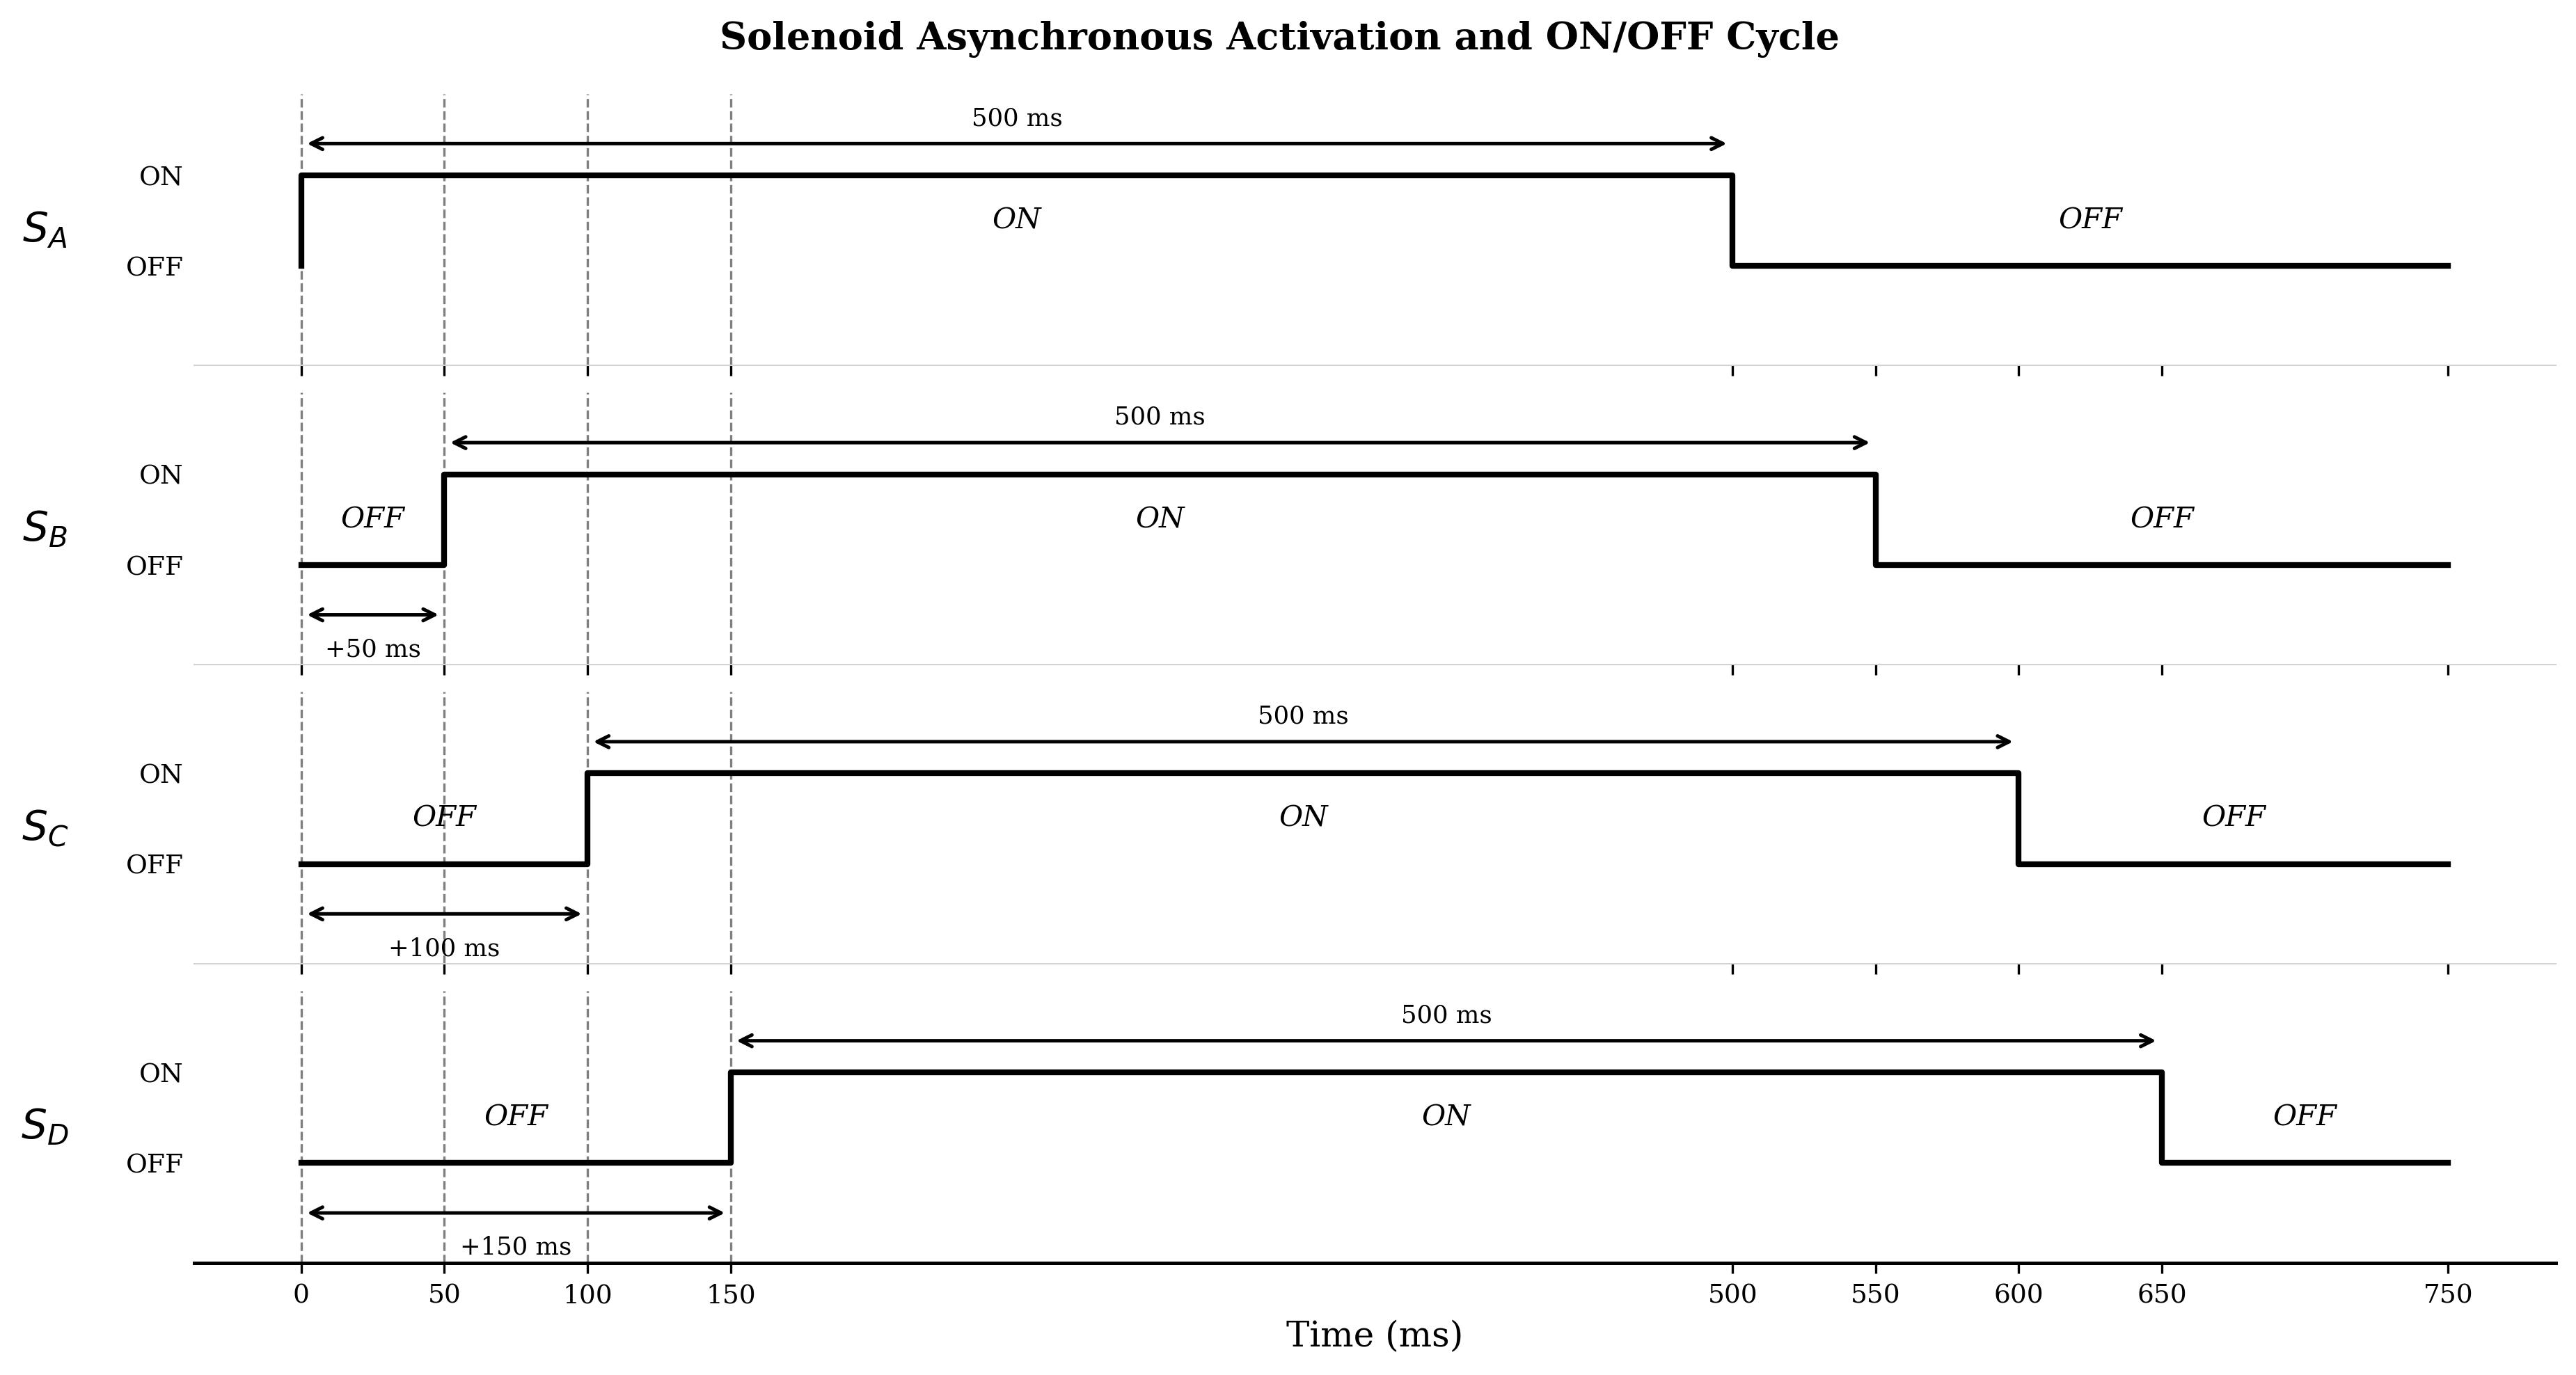
\includegraphics[width=0.95\textwidth]{Images/solenoid_timing.png}
    \caption{Timing diagram for the staggered asynchronous solenoid pulse protocol. Each solenoid ($S_A$ through $S_D$) activates sequentially with a 50\,ms inter-solenoid delay and remains active for 500\,ms. The complete four-solenoid cycle spans 650\,ms. The staggered pattern produces a travelling impulse wave across the tray, generating grain rotation and dispersion without interference between simultaneous activations.}
    \label{fig:solenoid_timing}
\end{figure}

%----------------------------------------------------------------------------------------
\section{Hardware Integration: The Hole-Fitting Mechanism}
%----------------------------------------------------------------------------------------

Having settled on solenoid actuation, the remaining design problem was the mechanical interface between the solenoid plungers and the sample tray. Poor coupling at this interface---any compliance, flex, or friction that absorbs part of the plunger stroke---converts a sharp impulse into a damped vibration. The grain bed responds accordingly: reduced de-clumping, reduced rotation, reduced diversity of captured orientations.

Two interface approaches were explored.

The first was a \textbf{drawer mechanism}: a pull-out tray on guide rails with magnetic retention. The ergonomic logic was reasonable---drawer mechanisms are familiar and reduce the cognitive overhead of loading a sample. In practice, it failed for two reasons. Magnetic retention was destabilised by the active solenoid magnetic fields, producing inconsistent retention force that was difficult to characterise and impossible to make reliable under all operating conditions. More critically, the guide rails introduced flex and friction that absorbed significant plunger energy, effectively undoing the impulse actuation strategy.

The second approach, which became the final design, was a \textbf{hole-fitting mechanism}: the tray has four precision apertures positioned to align with the solenoid plungers when the tray is seated. Plungers engage directly through the apertures on activation, creating near-rigid force transfer with minimal damping. The tray is loaded by placing it vertically onto the plunger array---a motion that is slightly less immediately intuitive than a drawer pull, but one that takes less than two seconds to perform and proved entirely unproblematic in user observation during the Bangalore demonstration.

The same design simplified maintenance. Tray removal and replacement requires only vertical motion---no rails to accumulate dust blockages, no fasteners, no tools.

%----------------------------------------------------------------------------------------
\section{Summary}
%----------------------------------------------------------------------------------------

The mechanical development described in this chapter is largely a record of following failure to its source. Vibration failed specifically---not generically---in ways that illuminated exactly what the dispersion mechanism needed to do differently. Solenoid impulse actuation with staggered timing addressed each of those failure modes directly, and the hole-fitting tray interface ensured that the energy intended for the grain bed actually reached it. The system that resulted converts a physically intractable dense-pile imaging problem into a tractable sequence-of-frames classification problem by making the required information enter the camera over time. Chapter~\ref{Chapter6} describes what happens to that information once it does.

%----------------------------------------------------------------------------------------
\section{Final Hardware Integration and Prototyping}
%----------------------------------------------------------------------------------------

With each subsystem validated independently---optoelectrical calibration, solenoid actuation, tray interface---the final stage was assembly of the high-fidelity prototype. This was not simply a matter of combining components. The spatial relationships between the solenoid array, the imaging surface, the LCD backlight, and the camera mount were all constrained by the impulse mechanics; if the tray moved too far from the camera focal plane under actuation, image sharpness would degrade during the most informative capture moments.

Figure~\ref{fig:final_integration} documents the physical assembly sequence: custom PCB fabrication, chassis assembly around the solenoid array, wiring, and the fully assembled device. The custom PCB consolidated solenoid driver circuits and GPIO timing into a single board, replacing a prototype breadboard arrangement that had proven unreliable in conditions of dust and physical vibration.

\begin{figure}[p]
    \centering
    \includegraphics[width=\textwidth,height=0.85\textheight,keepaspectratio]{final CAD exploded view.PNG}
    \caption{CAD exploded view of the Drishti device, showing the vertical component stack: optics module, electromagnetic actuation array, and control electronics within the aluminium chassis.}
    \label{fig:final_cad_full}
\end{figure}

\begin{figure}[H]
    \centering
    % Row 1: 3 images
    \begin{subfigure}[t]{0.32\textwidth}
        \centering
        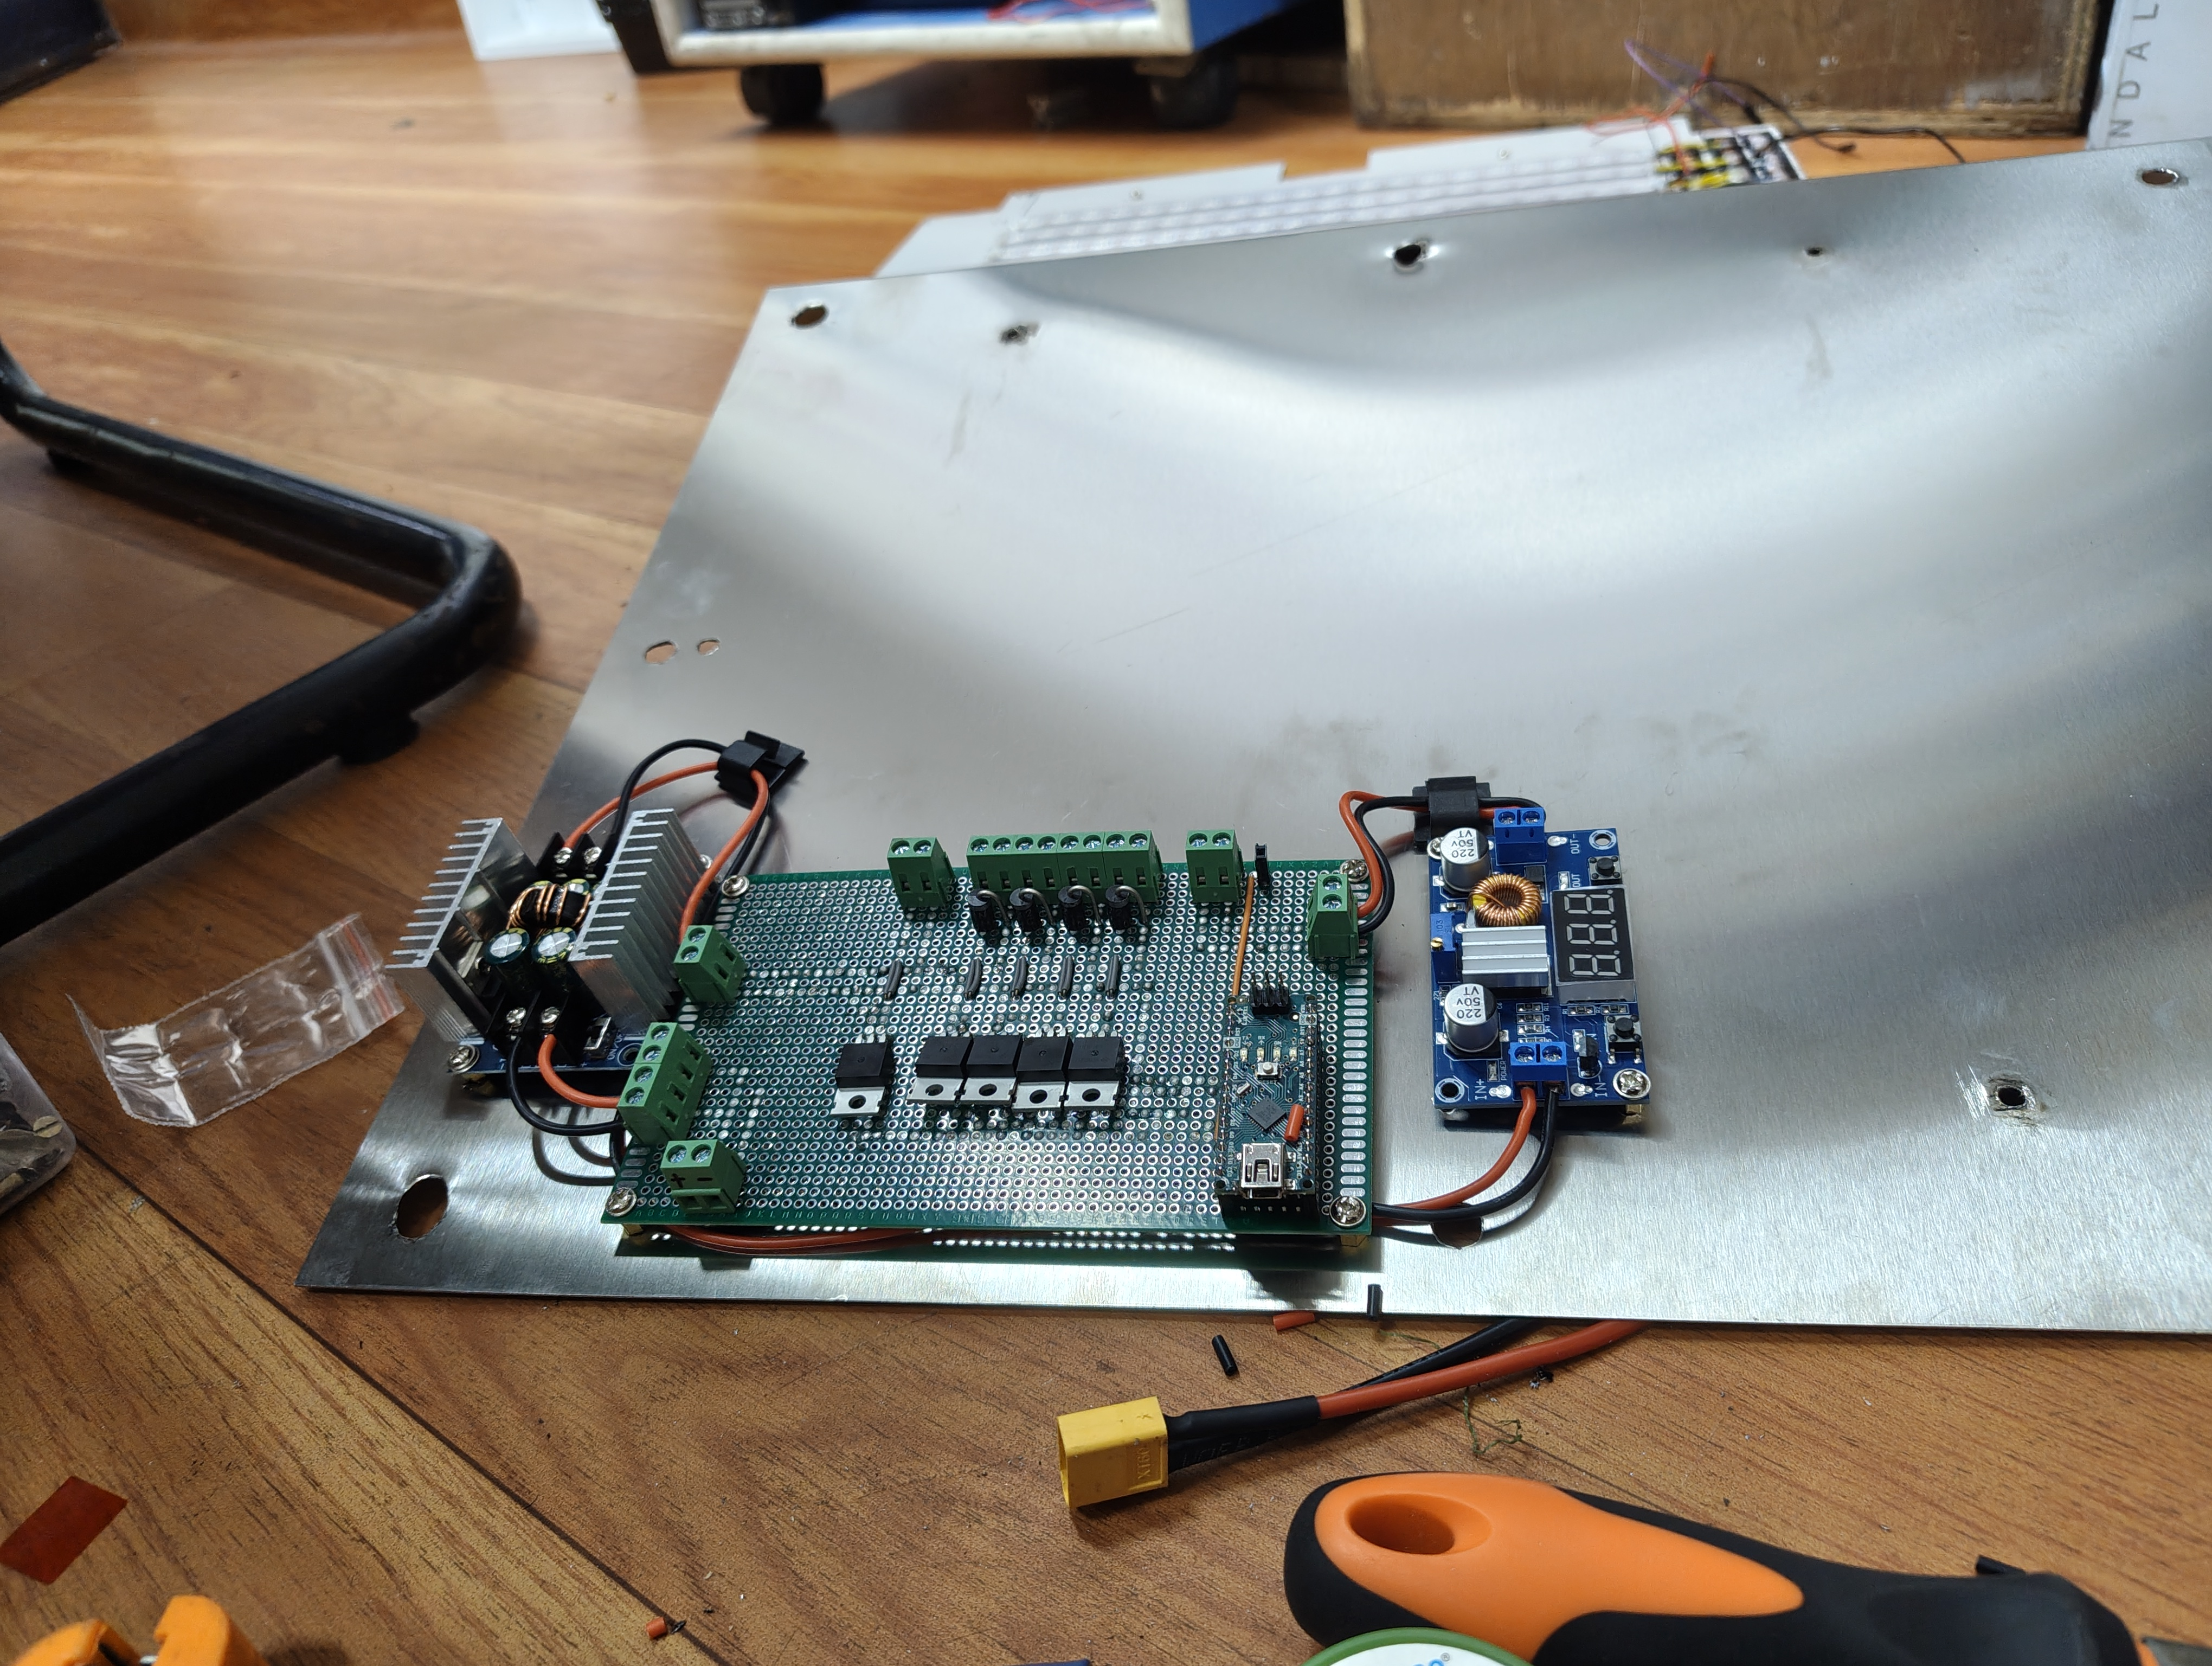
\includegraphics[width=\textwidth]{final PCB circuit.jpg}
        \caption{Custom PCB.}
        \label{fig:final_pcb}
    \end{subfigure}
    \hfill
    \begin{subfigure}[t]{0.32\textwidth}
        \centering
        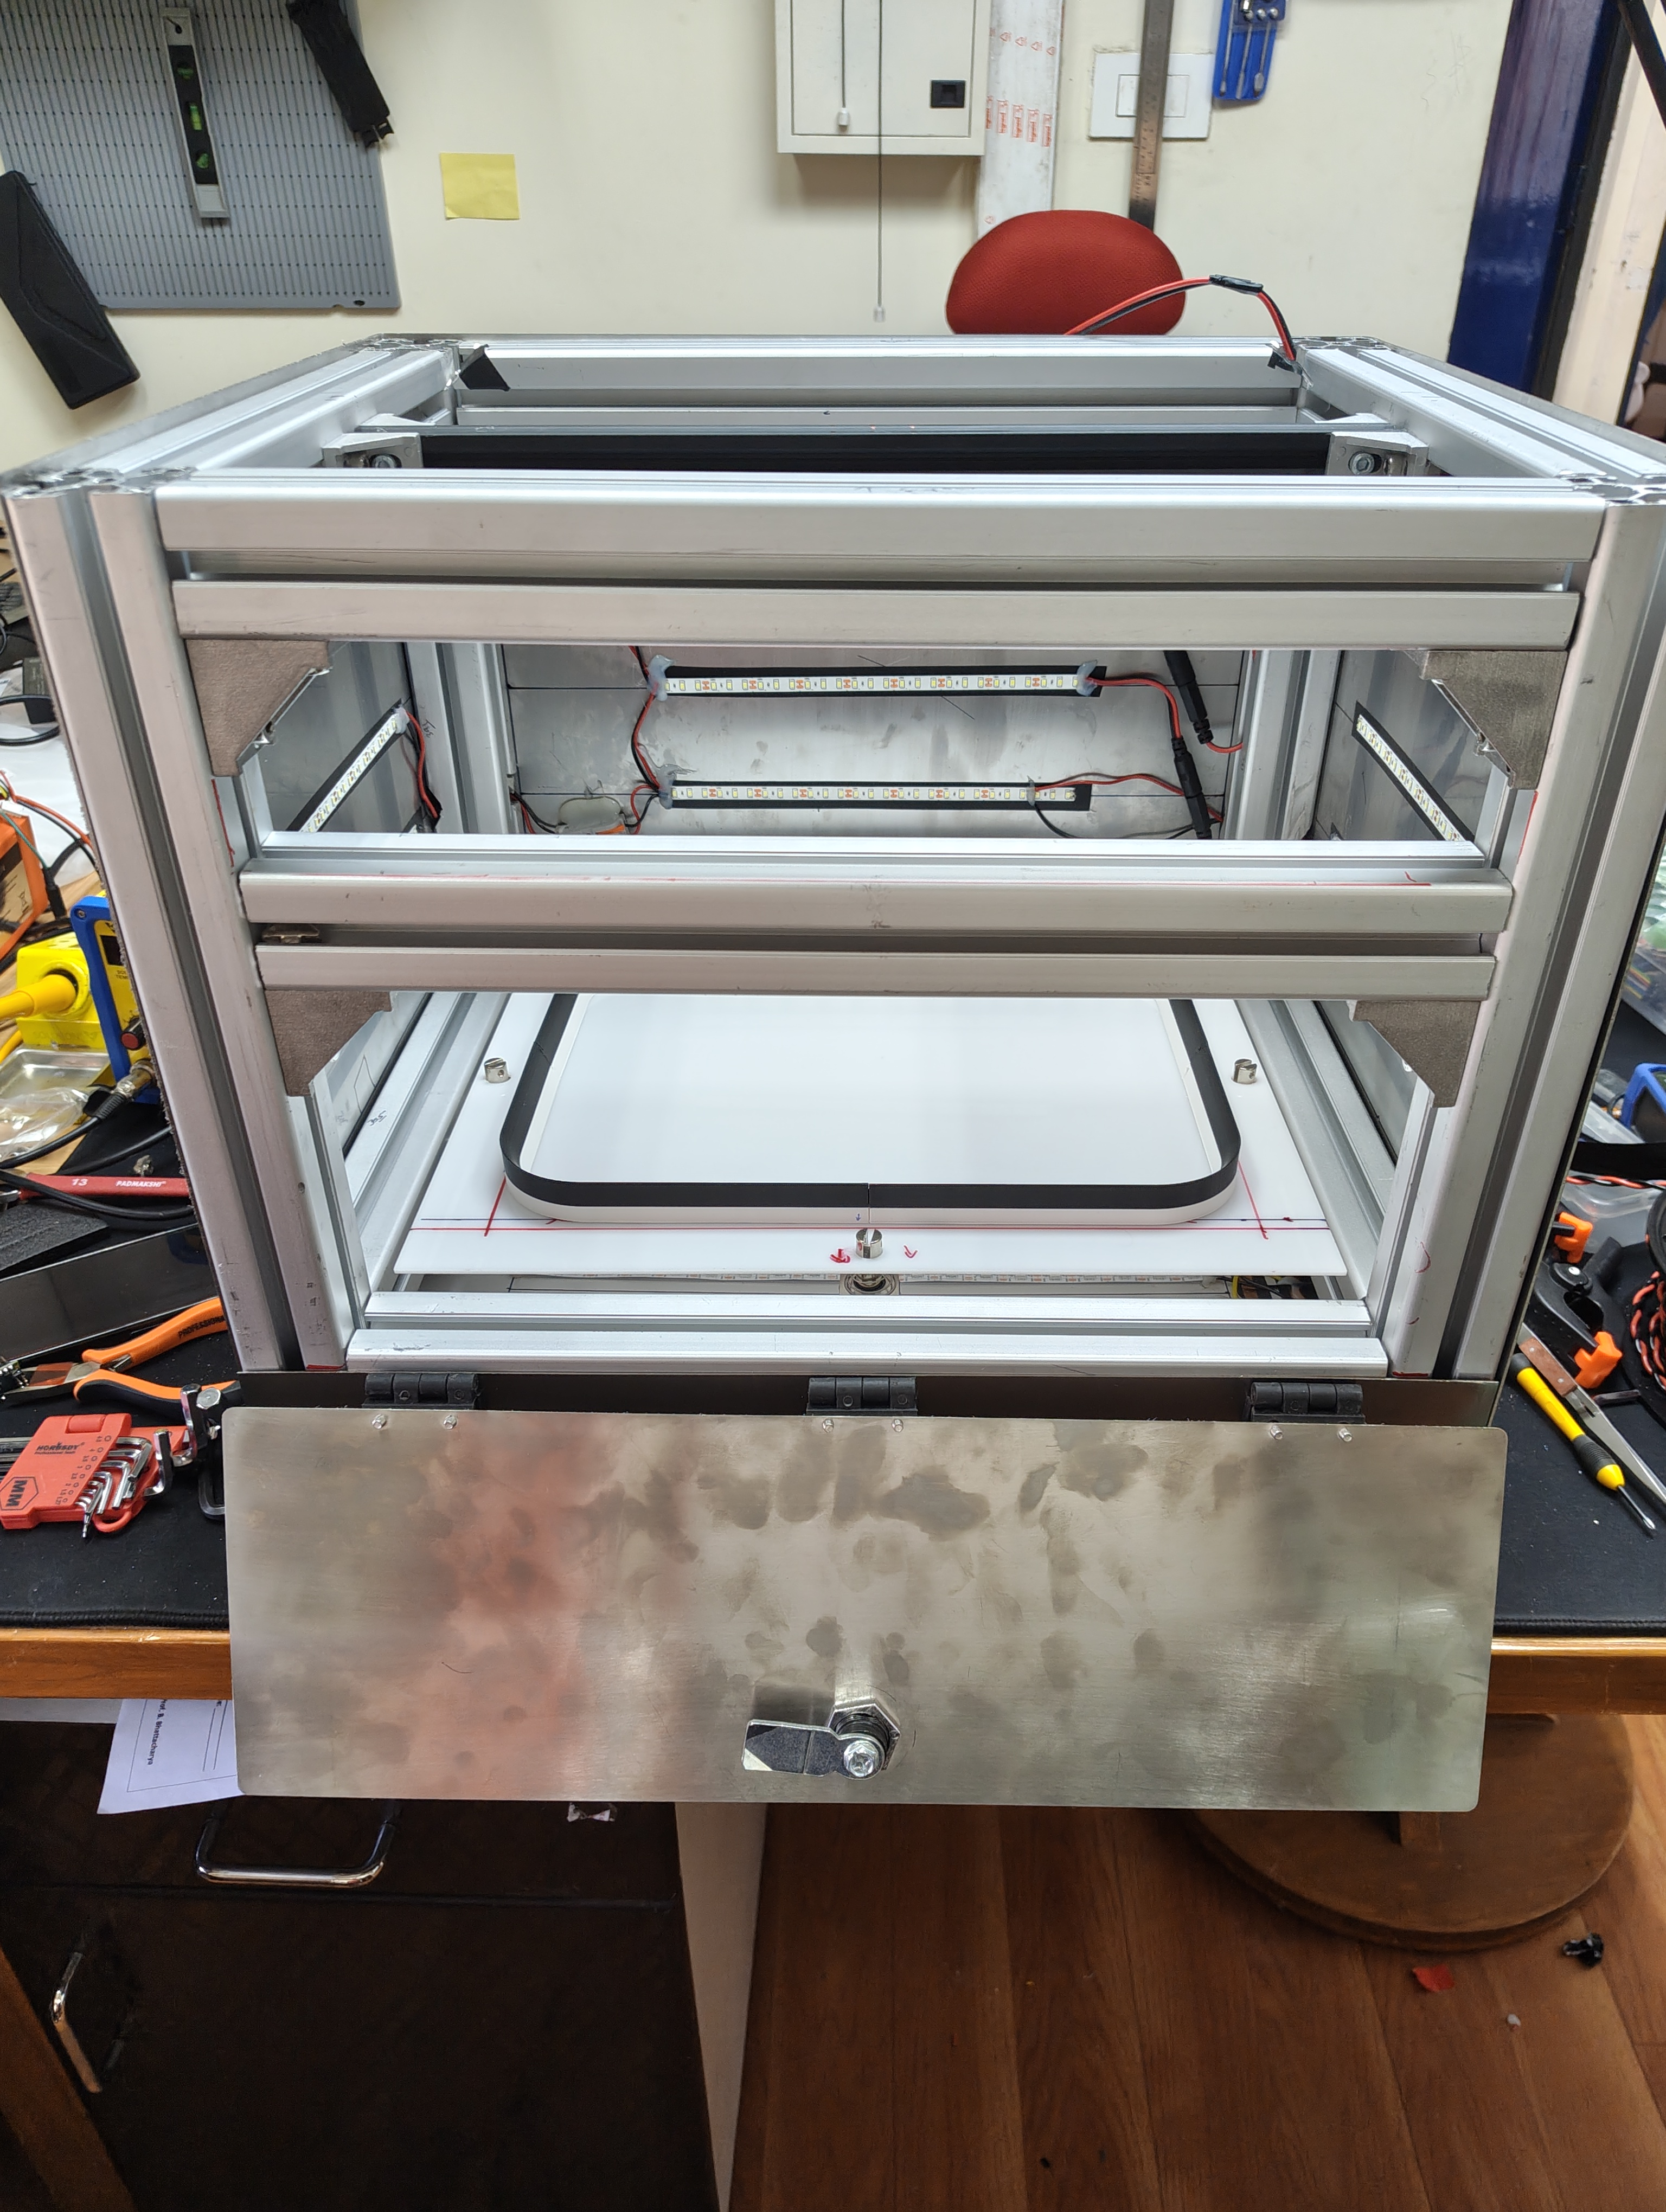
\includegraphics[width=\textwidth]{final prototype making 1.jpg}
        \caption{Chassis assembly.}
        \label{fig:final_proto_1}
    \end{subfigure}
    \hfill
    \begin{subfigure}[t]{0.32\textwidth}
        \centering
        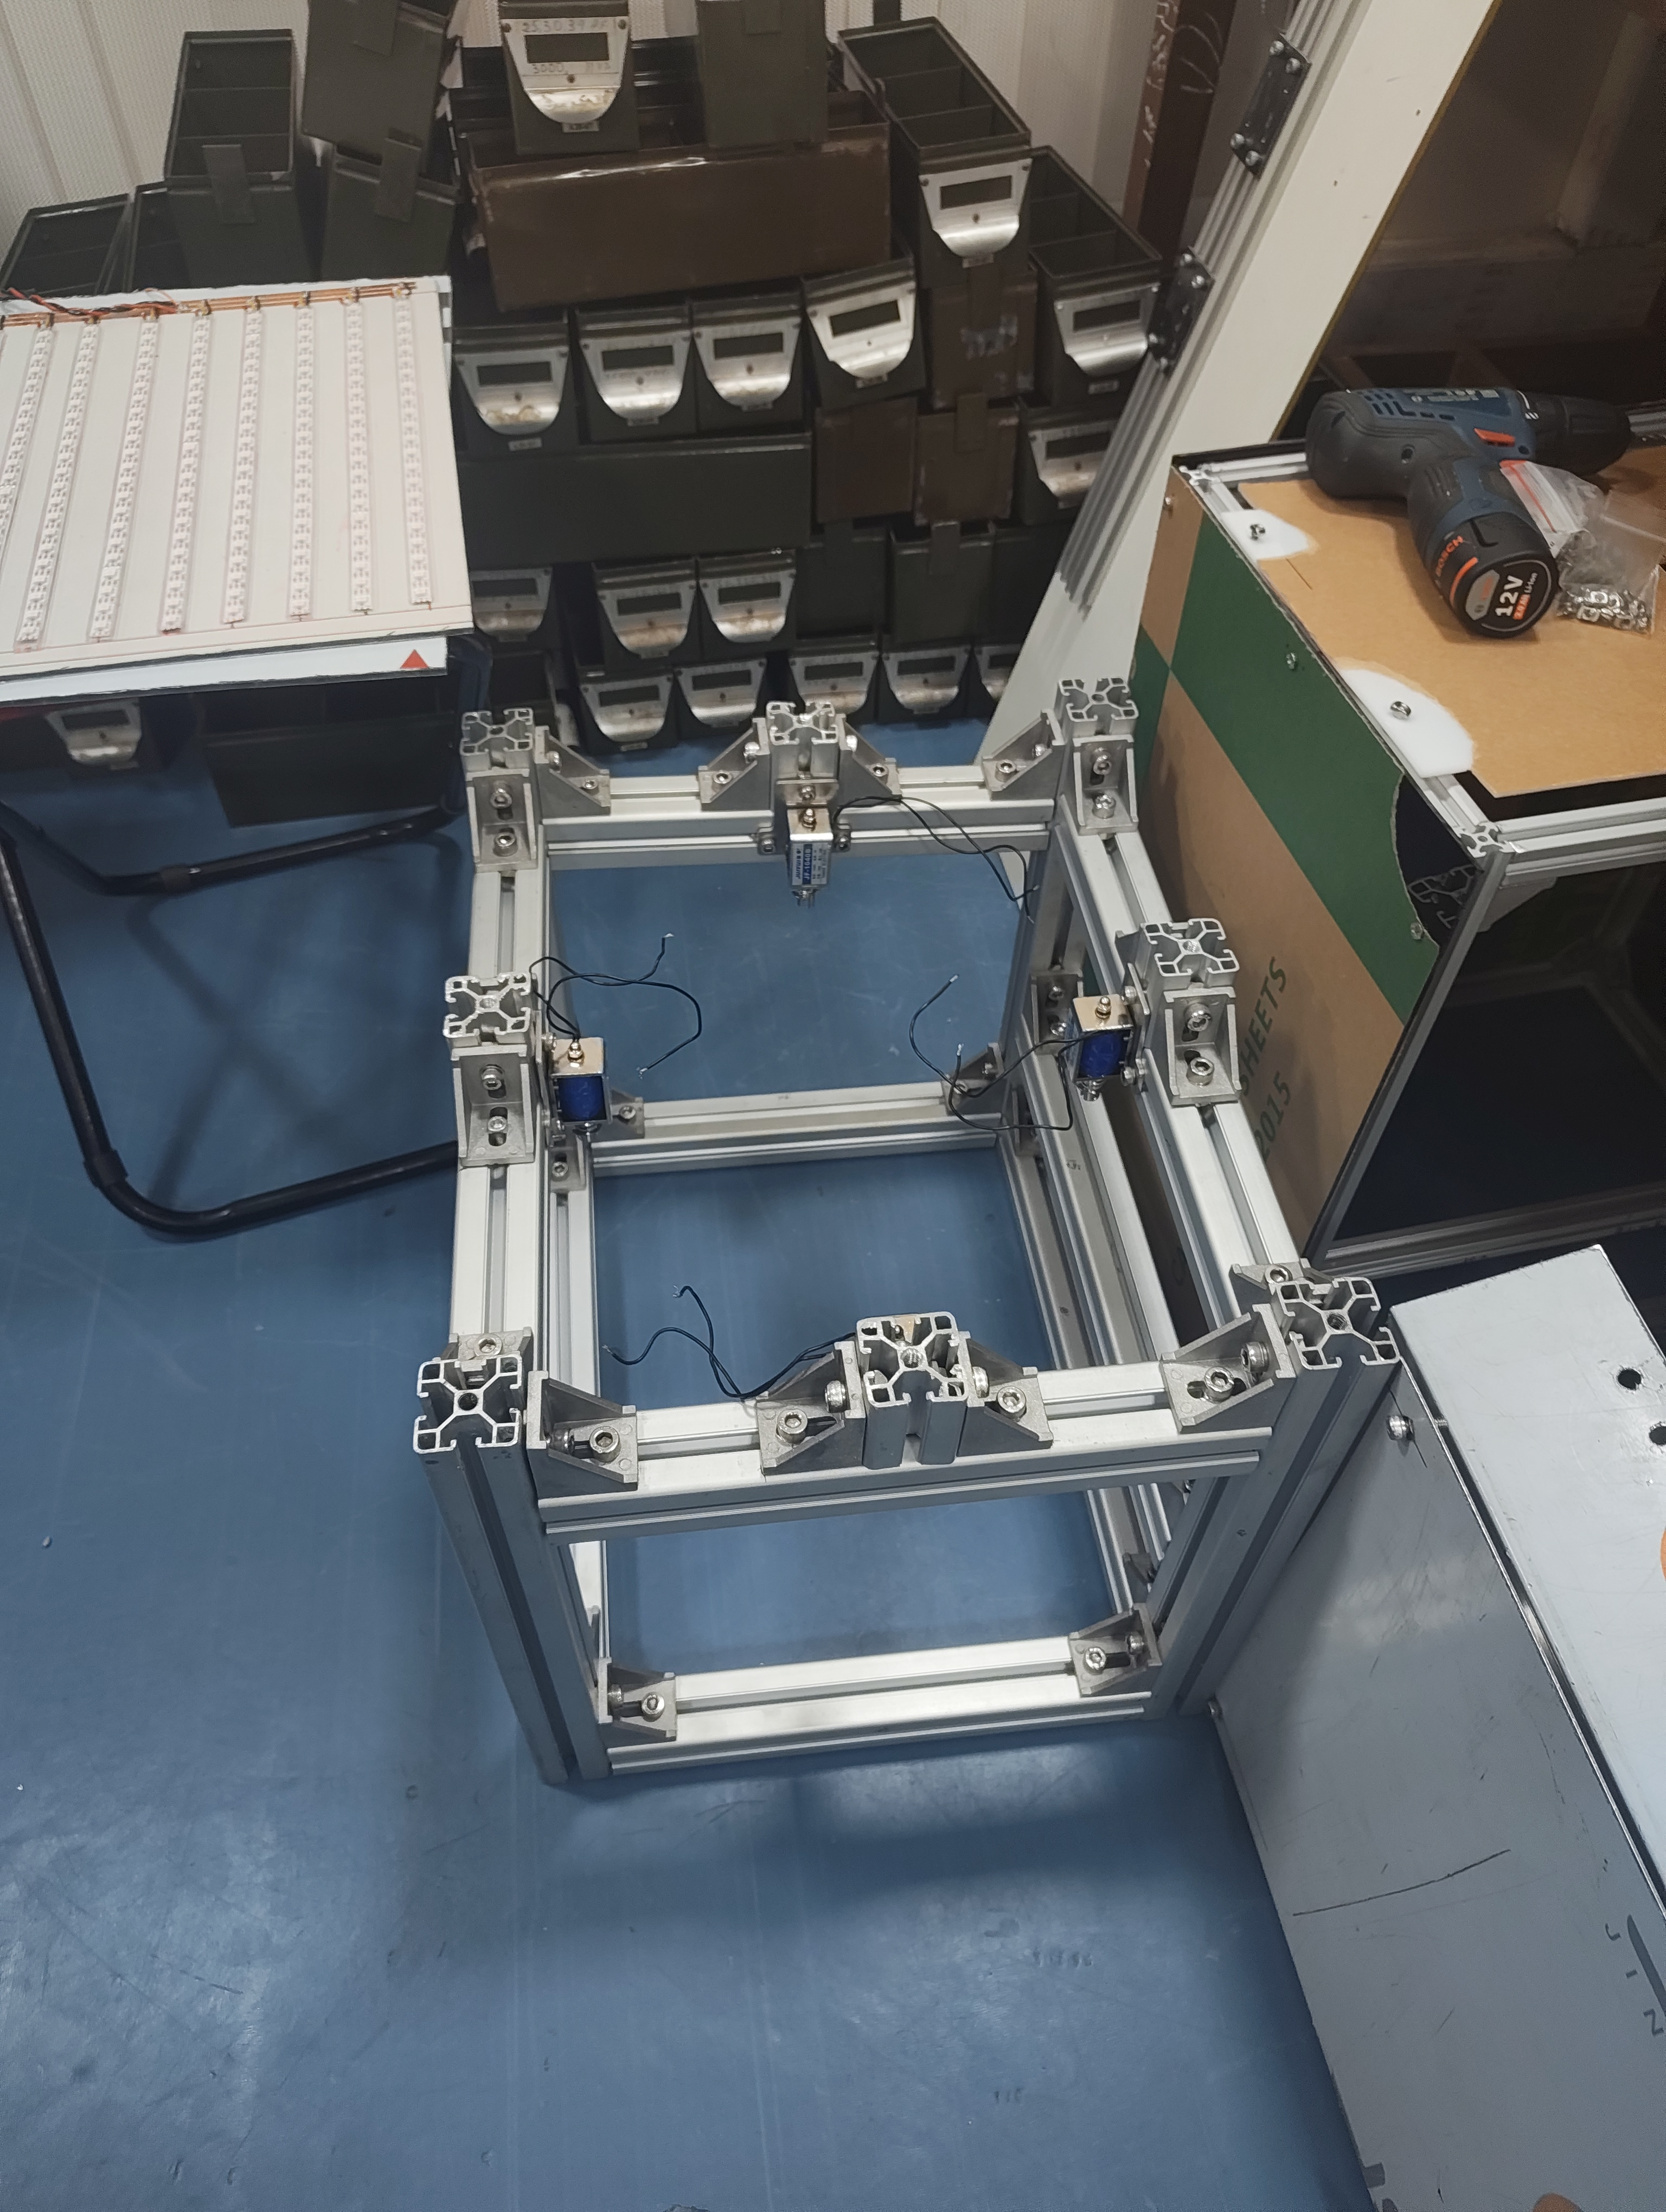
\includegraphics[width=\textwidth]{final prototype making 2.jpg}
        \caption{Solenoid mounting.}
        \label{fig:final_proto_2}
    \end{subfigure}
    
    \vspace{2em}
    
    % Row 2: 2 images, centered
    \begin{subfigure}[t]{0.32\textwidth}
        \centering
        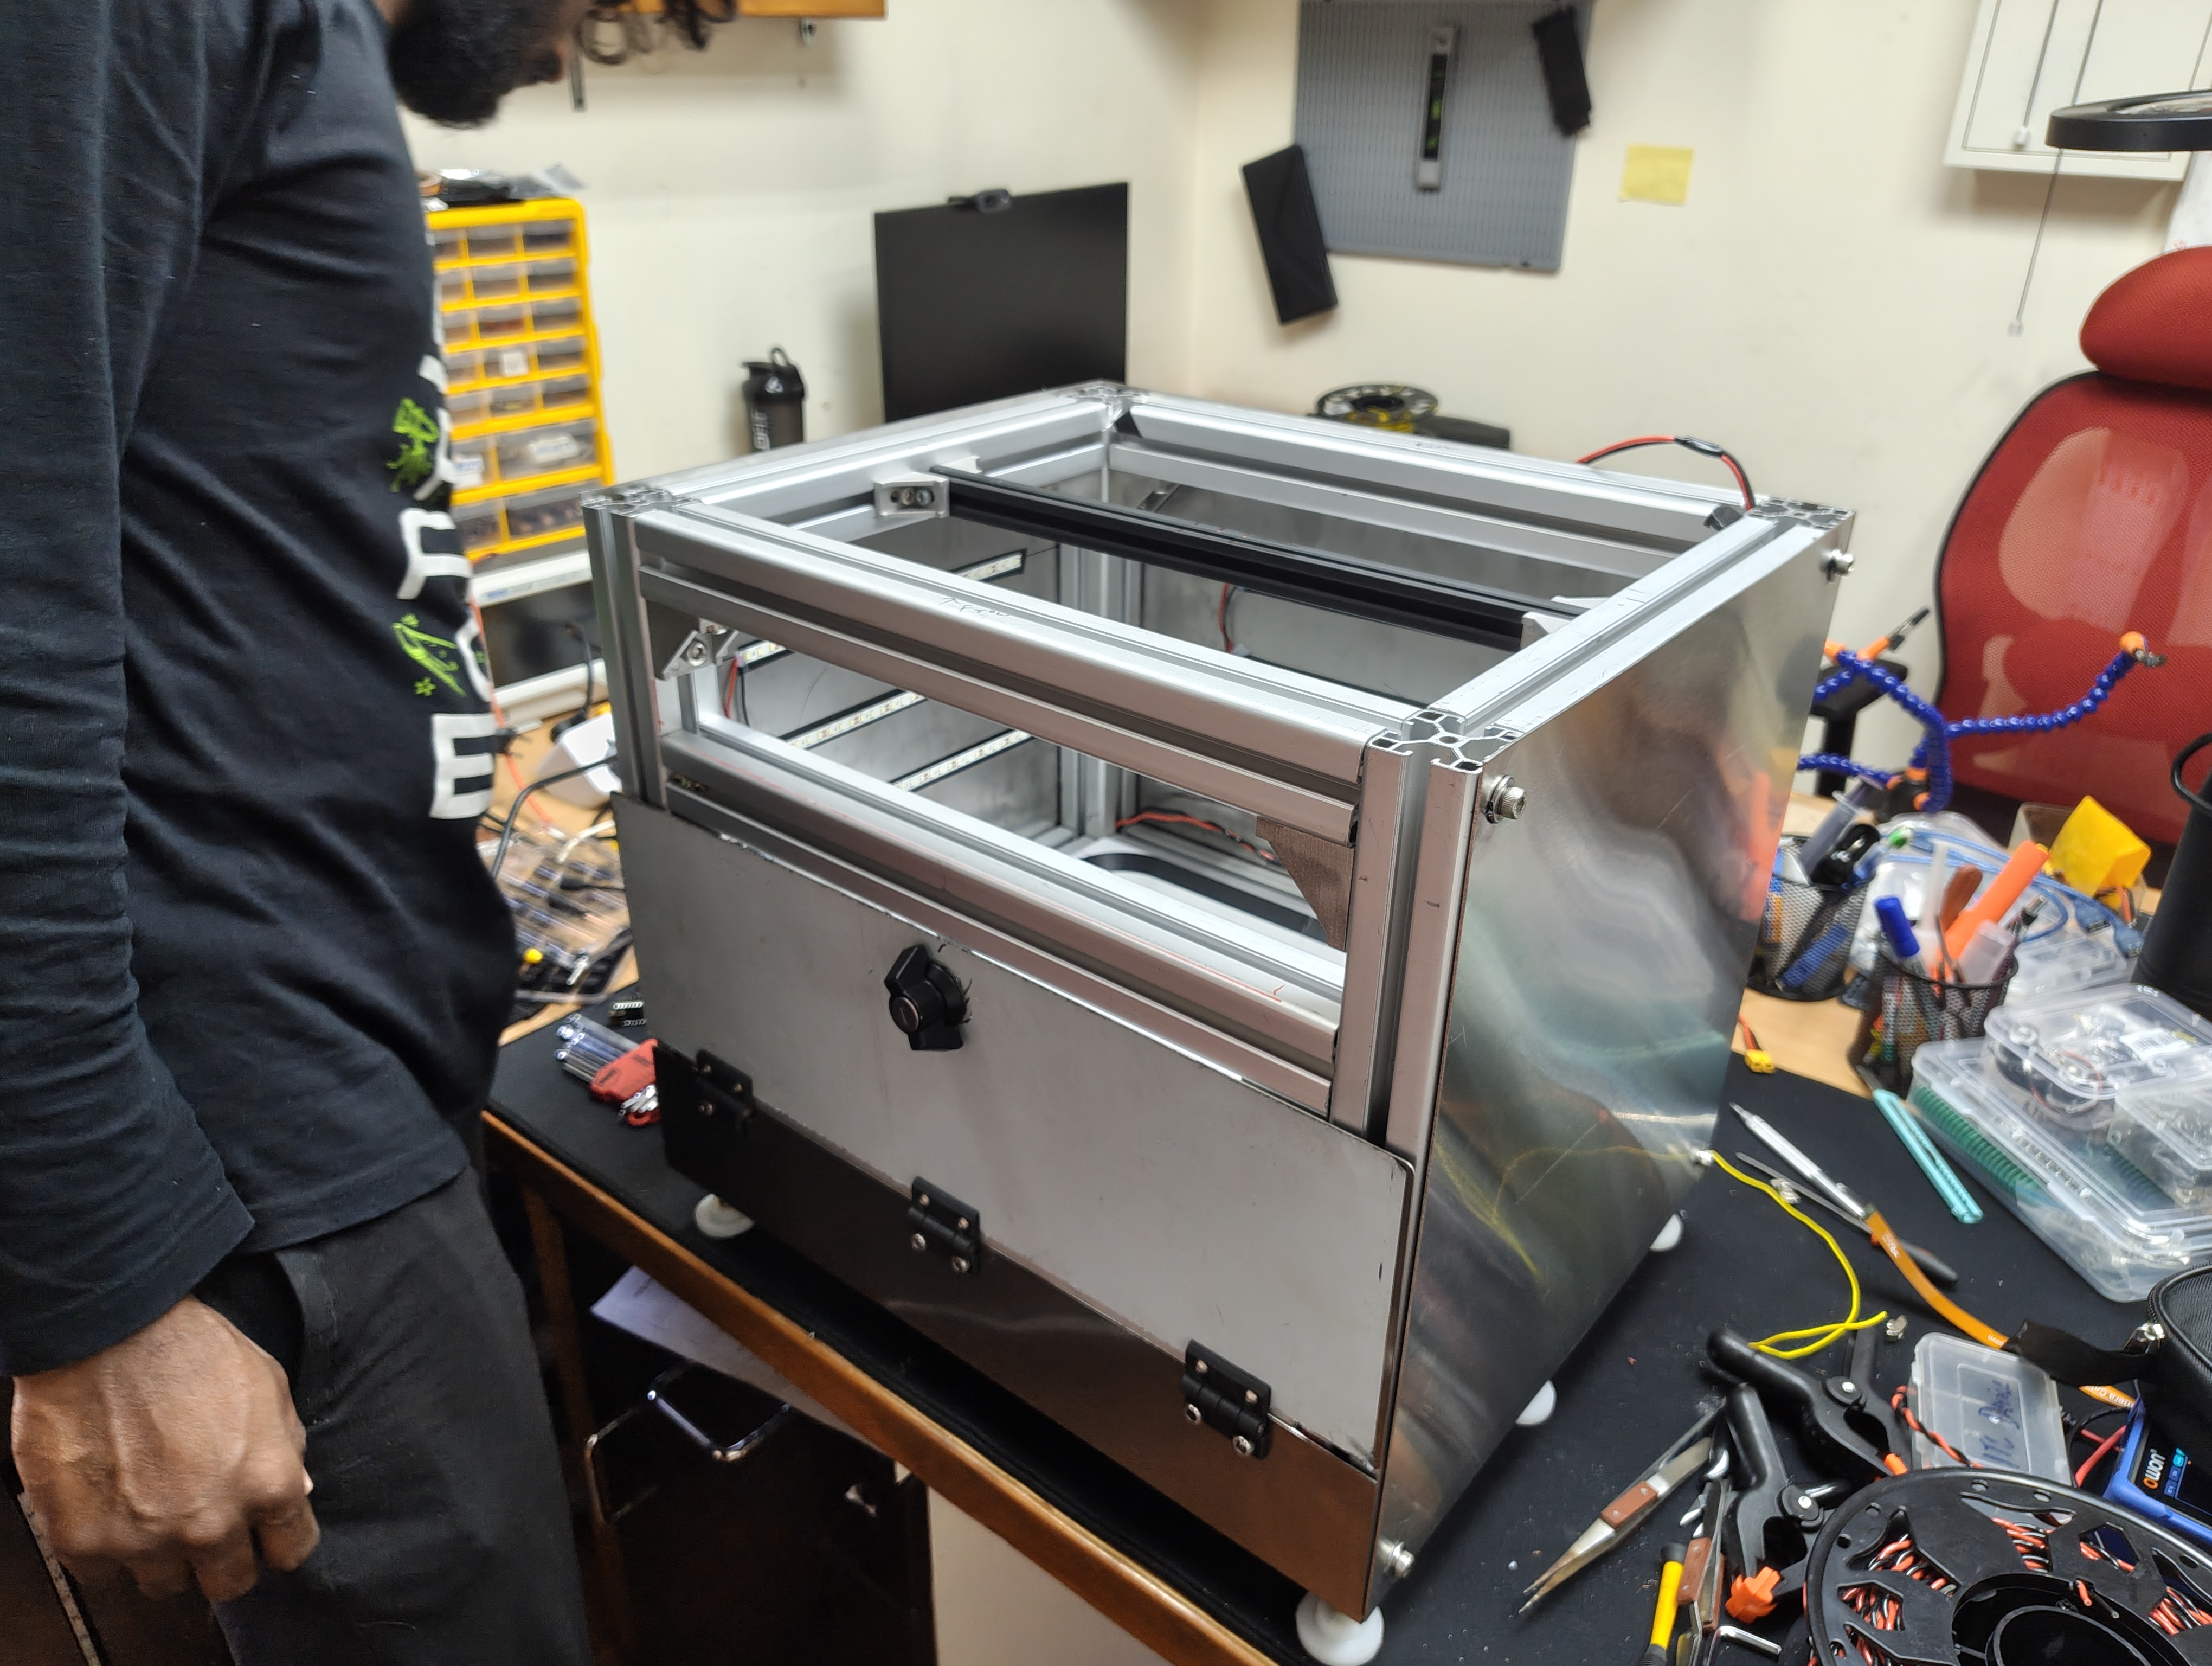
\includegraphics[width=\textwidth]{final prototype making 3.jpg}
        \caption{Hardware wiring.}
        \label{fig:final_proto_3}
    \end{subfigure}
    \hspace{0.05\textwidth}
    \begin{subfigure}[t]{0.32\textwidth}
        \centering
        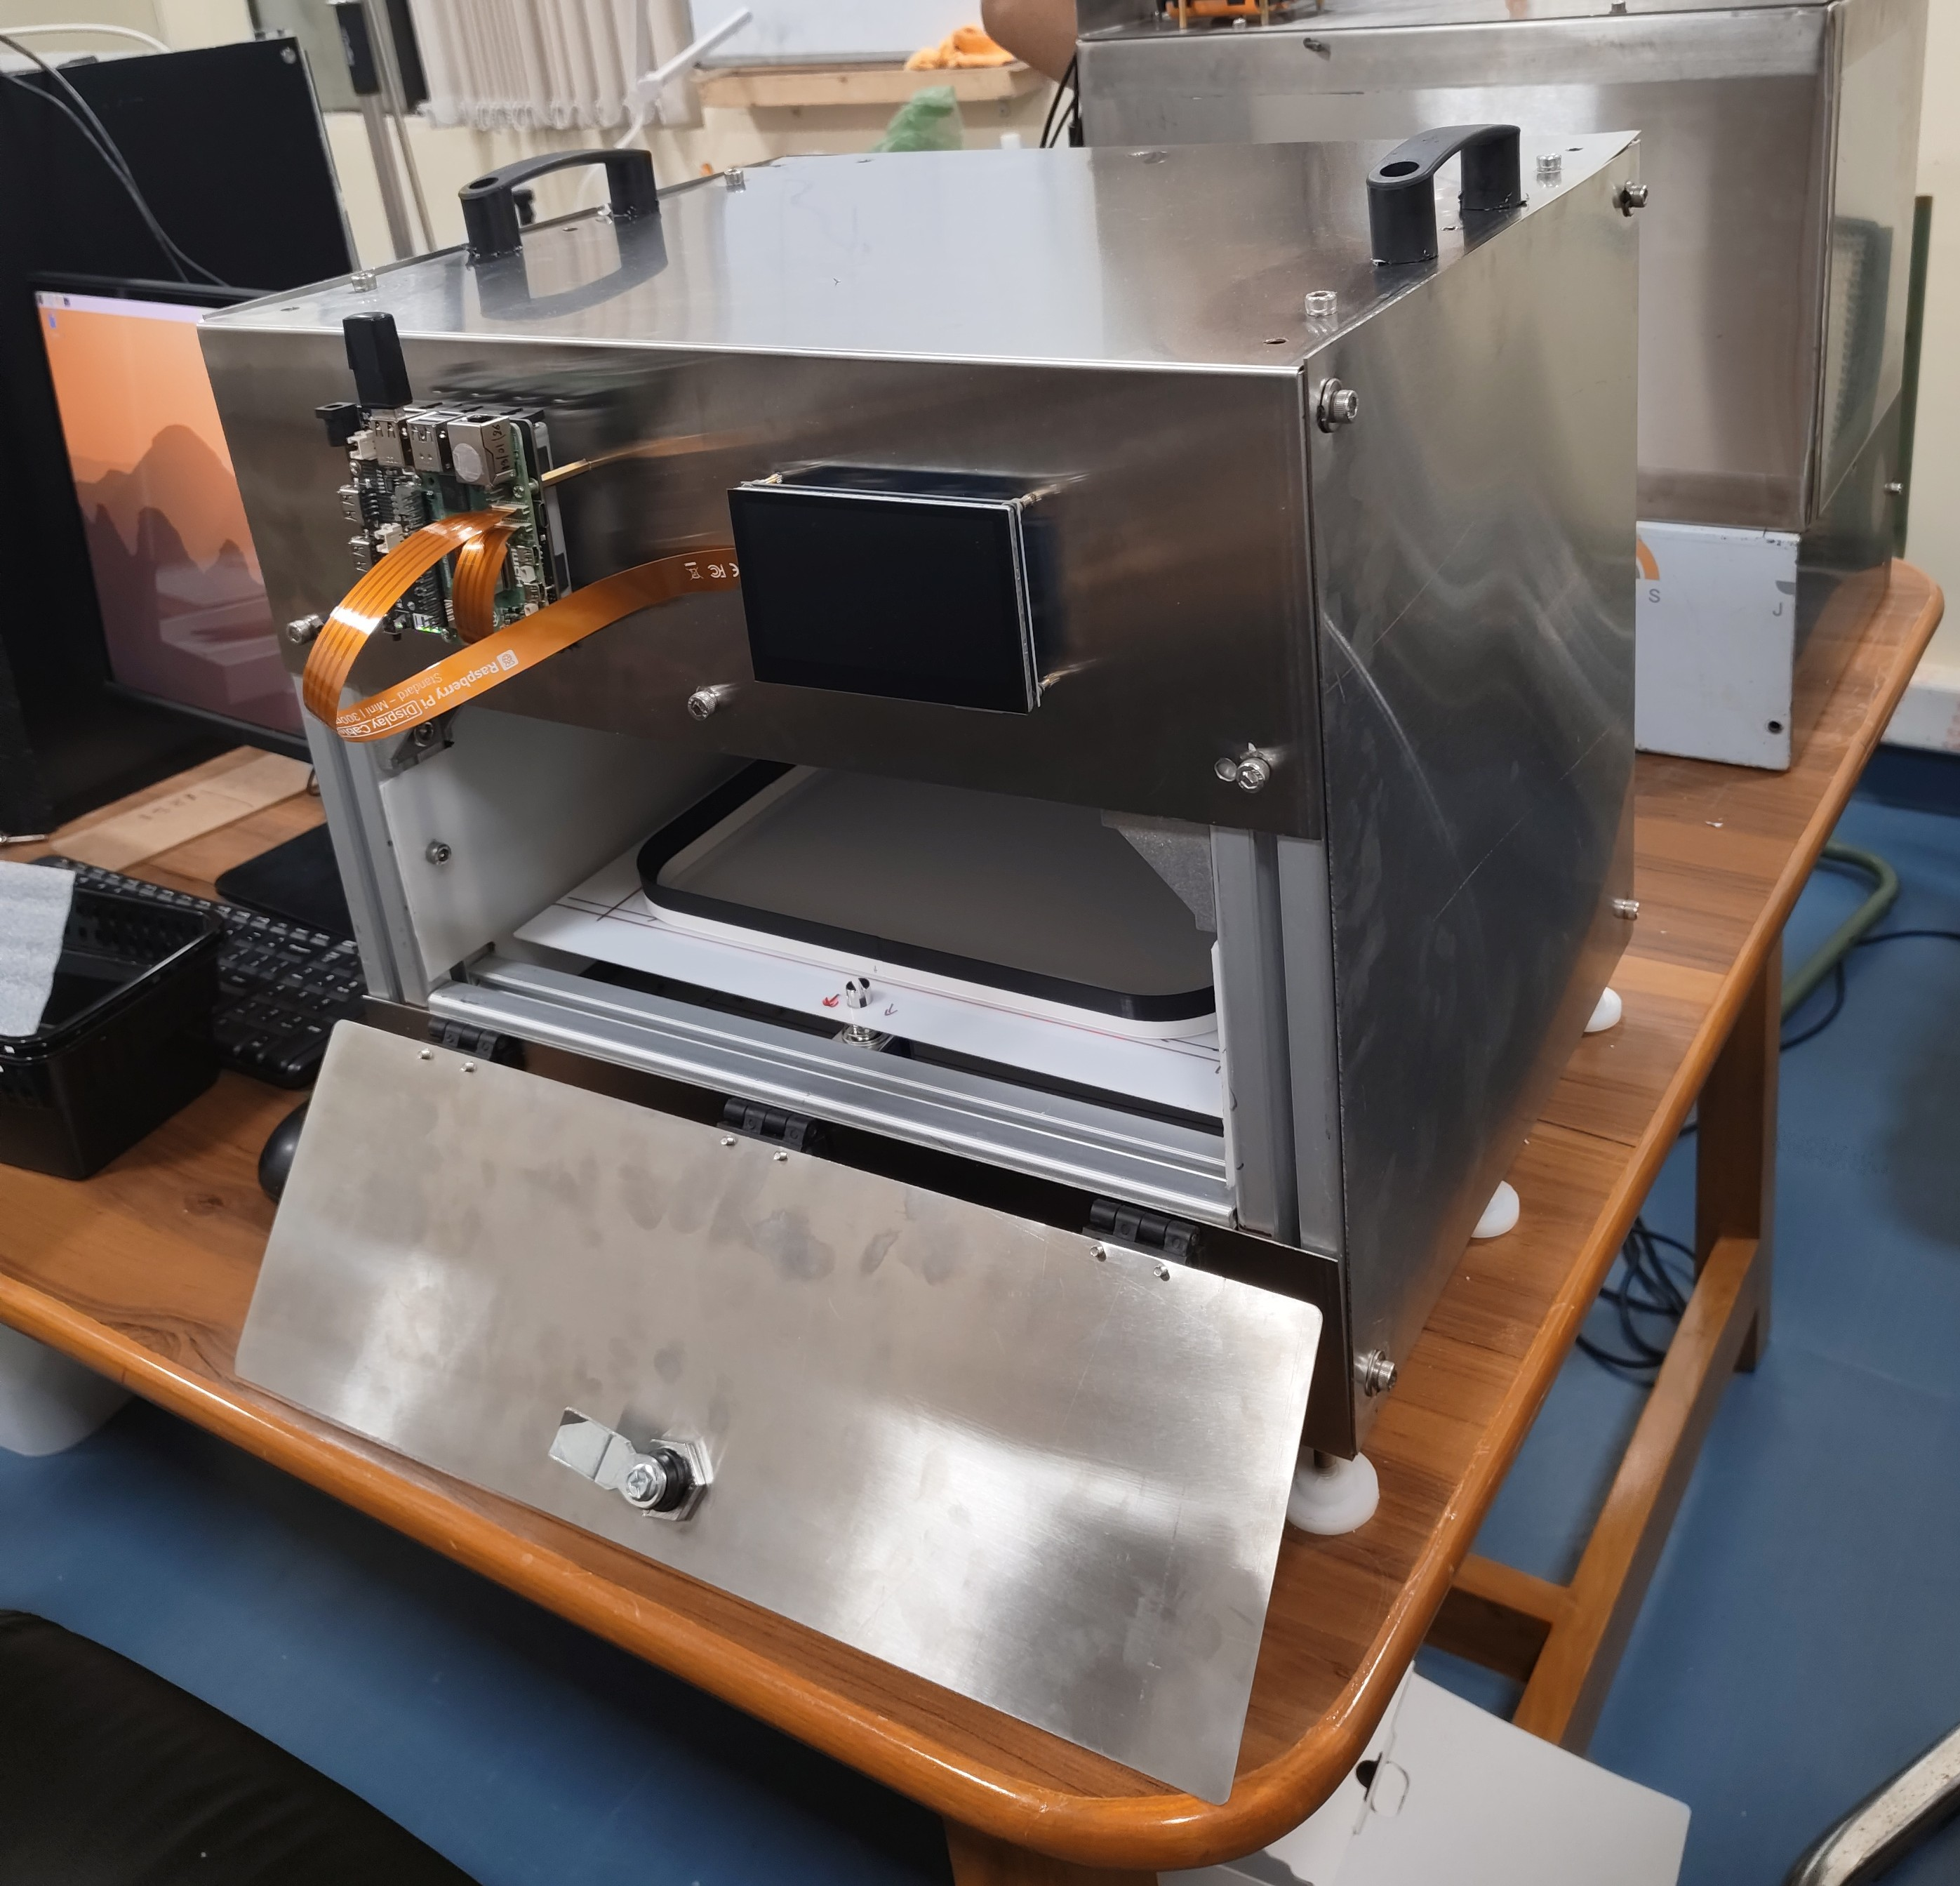
\includegraphics[width=\textwidth]{final prototype photo.jpg}
        \caption{Fully assembled.}
        \label{fig:final_proto_photo}
    \end{subfigure}

    \caption{Physical assembly sequence of the final prototype. (a)~Custom PCB for solenoid pulse timing. (b--d)~Progressive chassis and electronics assembly. (e)~Completed device prepared for deployment.}
    \label{fig:final_integration}
\end{figure}
 
% Chapter 6 --- Computational Architecture

\chapter{The Computational Architecture: From Pixel to Procurement Decision}\doublespacing
\label{Chapter6}
\lhead{Chapter V. \emph{Computational Architecture}}

%----------------------------------------------------------------------------------------
\section{Optoelectrical Parameter Optimisation}
%----------------------------------------------------------------------------------------

Auto White Balance (AWB) was identified as the primary source of chromatic instability in the imaging pipeline. AWB is designed for consumer photography, where the goal is perceptually natural colour rendering. In this application, that correction is counterproductive. The chromatic signals that AWB suppresses (subtle colour differences between \textit{Kernel Burnt} and dark-variety \textit{Pure Wheat}, early \textit{Black Tip} discolouration, and the surface sheen of \textit{Infested} grain) are the diagnostic cues the model depends on.

AWB was disabled and replaced with a fixed white-balance matrix calibrated under Drishti's specific illumination using a standard colour reference chart. Shutter speed was tuned to balance motion suppression during post-actuation grain settling against exposure level. WS2812B LED output was adjusted spatially to reduce specular reflections on glossy kernel surfaces \cite{LiWheat2024, ElMasry2019}. The result is a stable, repeatable optical signal: the same grain photographed across ten successive frames produces chromatically consistent images.

%----------------------------------------------------------------------------------------
\section{Dataset Acquisition and ML Model Training}
%----------------------------------------------------------------------------------------

% Note to author: Specific model architecture details, accuracy figures, and training
% hyperparameters should be completed once final training runs are concluded.

Public grain datasets do not represent the procurement network's specific wheat varieties, Drishti's illumination profile, or the partially dispersed sample states the device produces. Deploying a model trained on a generic dataset in a specific physical system introduces dataset shift, which tends to produce confident misclassification rather than uncertain prediction \cite{QuinoneroCandela2009}.

A domain-specific dataset was therefore built from scratch, capturing images through the same optical and mechanical pipeline described in Chapters~\ref{Chapter4} and~\ref{Chapter5}. Grain specimens were annotated across all twelve categories. Particular attention was given to the confusable pairs identified in fieldwork as most error-prone: \textit{Kernel Burnt} versus dark-variety \textit{Pure Wheat}, early \textit{Infested} versus \textit{Broken}, and \textit{Potia} versus immature \textit{Pure Wheat}.

Instance segmentation was selected over bounding-box detection. The $W/W\%$ calculation requires area estimation per category. Pixel-level masks produce more accurate area measurements than bounding boxes, which systematically overestimate the area of irregularly shaped grain bodies.

%----------------------------------------------------------------------------------------
\section{Edge-to-Server Software Architecture}
%----------------------------------------------------------------------------------------

\subsection{System Architecture Overview}

The Raspberry Pi 5 handles actuation control, GPIO timing, and image capture efficiently. It is not suited to running production-scale instance segmentation inference within the five-minute cycle target. A server-client architecture was adopted.

\begin{figure}[H]
    \centering
    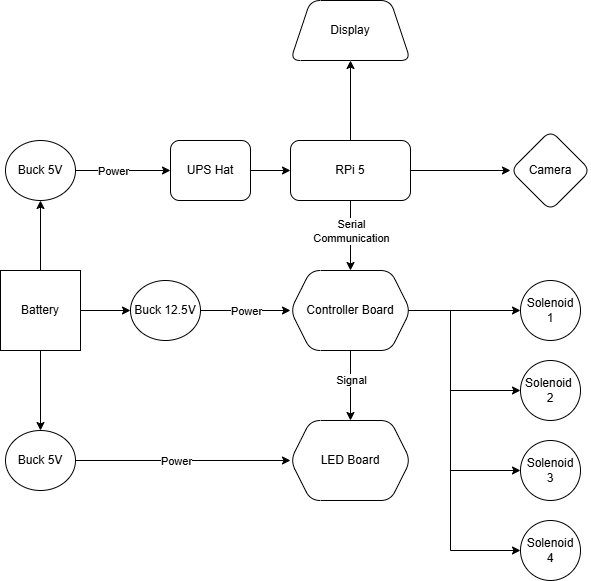
\includegraphics[width=0.9\textwidth]{Images/Drishti Hardware Architecture drawio.png}
    \caption{Drishti system architecture: the Raspberry Pi 5 edge node handles physical actuation and image capture; the central inference server handles segmentation and returns per-category $W/W\%$ results.}
    \label{fig:hardware_architecture}
\end{figure}

The Raspberry Pi 5 acts as the edge node: it manages actuation sequencing, captures images at calibrated parameters, applies lightweight preprocessing (resizing, calibration transforms, frame selection), and renders the local user interface. Preprocessed frames are transmitted over a local network to a central inference service. The service, exposed through a FastAPI endpoint, runs the instance segmentation model and returns per-category counts and $W/W\%$ values within the sub-five-minute window.

Running inference on a managed server allows model updates to be deployed centrally without physical access to field devices. Docker containerisation ensures consistent behaviour across the heterogeneous IT environments found at procurement sites \cite{Merkel2014}.

% Chapter 7 --- Human-Device Interaction

\chapter{Human-Device Interaction and User Experience Design}\doublespacing
\label{Chapter7}
\lhead{Chapter VI. \emph{Human-Device Interaction}}

%----------------------------------------------------------------------------------------
\section{Designing for the High-Pressure Industrial Environment}
%----------------------------------------------------------------------------------------

There is a particular challenge in designing for an industrial environment that looks, from the outside, like a straightforward usability problem but is not. The task that Drishti is meant to support---wheat quality assessment---is already being performed. It is being performed by experienced people who have developed their own workflows, their own shortcuts, and their own sense of what a good result looks like. Any new device enters that context not as a blank slate but as something that must earn its place in a routine that is already functional.

The fieldwork described in Chapter~\ref{Chapter2} made this concrete. Operators at the warehouse site were managing a queue of trucks, working with fine dust on every surface, handling grain in conditions that would be physically demanding even without the cognitive load of simultaneous classification and recording. The interaction model for Drishti was designed against that reality, not against a controlled user-testing scenario \cite{Stanton2005}. Norman's framework for design under real operating conditions \cite{Norman2013} provided a useful conceptual anchor: the goal is to reduce the number of decisions the operator has to make explicitly, not to eliminate their agency.

Two distinct interaction layers were addressed. The physical layer covers the tactile and procedural aspects of loading, unloading, and maintaining the device---everything that happens before and after an assessment. The digital layer covers how the system communicates during and after inference: what information is shown, in what order, and what actions the operator is expected to take.

%----------------------------------------------------------------------------------------
\section{Iterative Design of the Physical Interface}
%----------------------------------------------------------------------------------------

\subsection{The Problem of the Grain Tray}

The grain tray is loaded and unloaded with every assessment. In a busy procurement shift, that could happen thirty or forty times. A mechanism that takes fifteen seconds to operate rather than five does not seem like a significant difference until it is multiplied across a working day and a working season. The tray interface therefore received more design attention than its apparent simplicity might suggest.

The first iteration was a drawer mechanism with guide rails and magnetic retention. The logic was straightforward: drawer mechanisms are universally familiar, and the pull-out motion is intuitive enough that no instruction is required. It was rejected for reasons described in Chapter~\ref{Chapter5}---magnetic retention was destabilised by active solenoid fields, and the rails introduced enough compliance to damp the impulse actuation that the system depended on. A third problem emerged during field evaluation: dust. The rail channels accumulated fine wheat dust over repeated use, progressively increasing the friction that needed to be overcome on each opening. After a full shift, the drawer that had operated smoothly in the morning required deliberate force to open.

The finalised design uses a vertical placement approach: the operator loads grain onto the tray and places the tray directly downward onto four plunger apertures in the device surface. The motion is not intuitively obvious before instruction, but it takes under three seconds once learned and involves no moving parts beyond the tray itself. Nothing accumulates dust because there are no channels for it to accumulate in.

\begin{figure}[H]
    \centering
    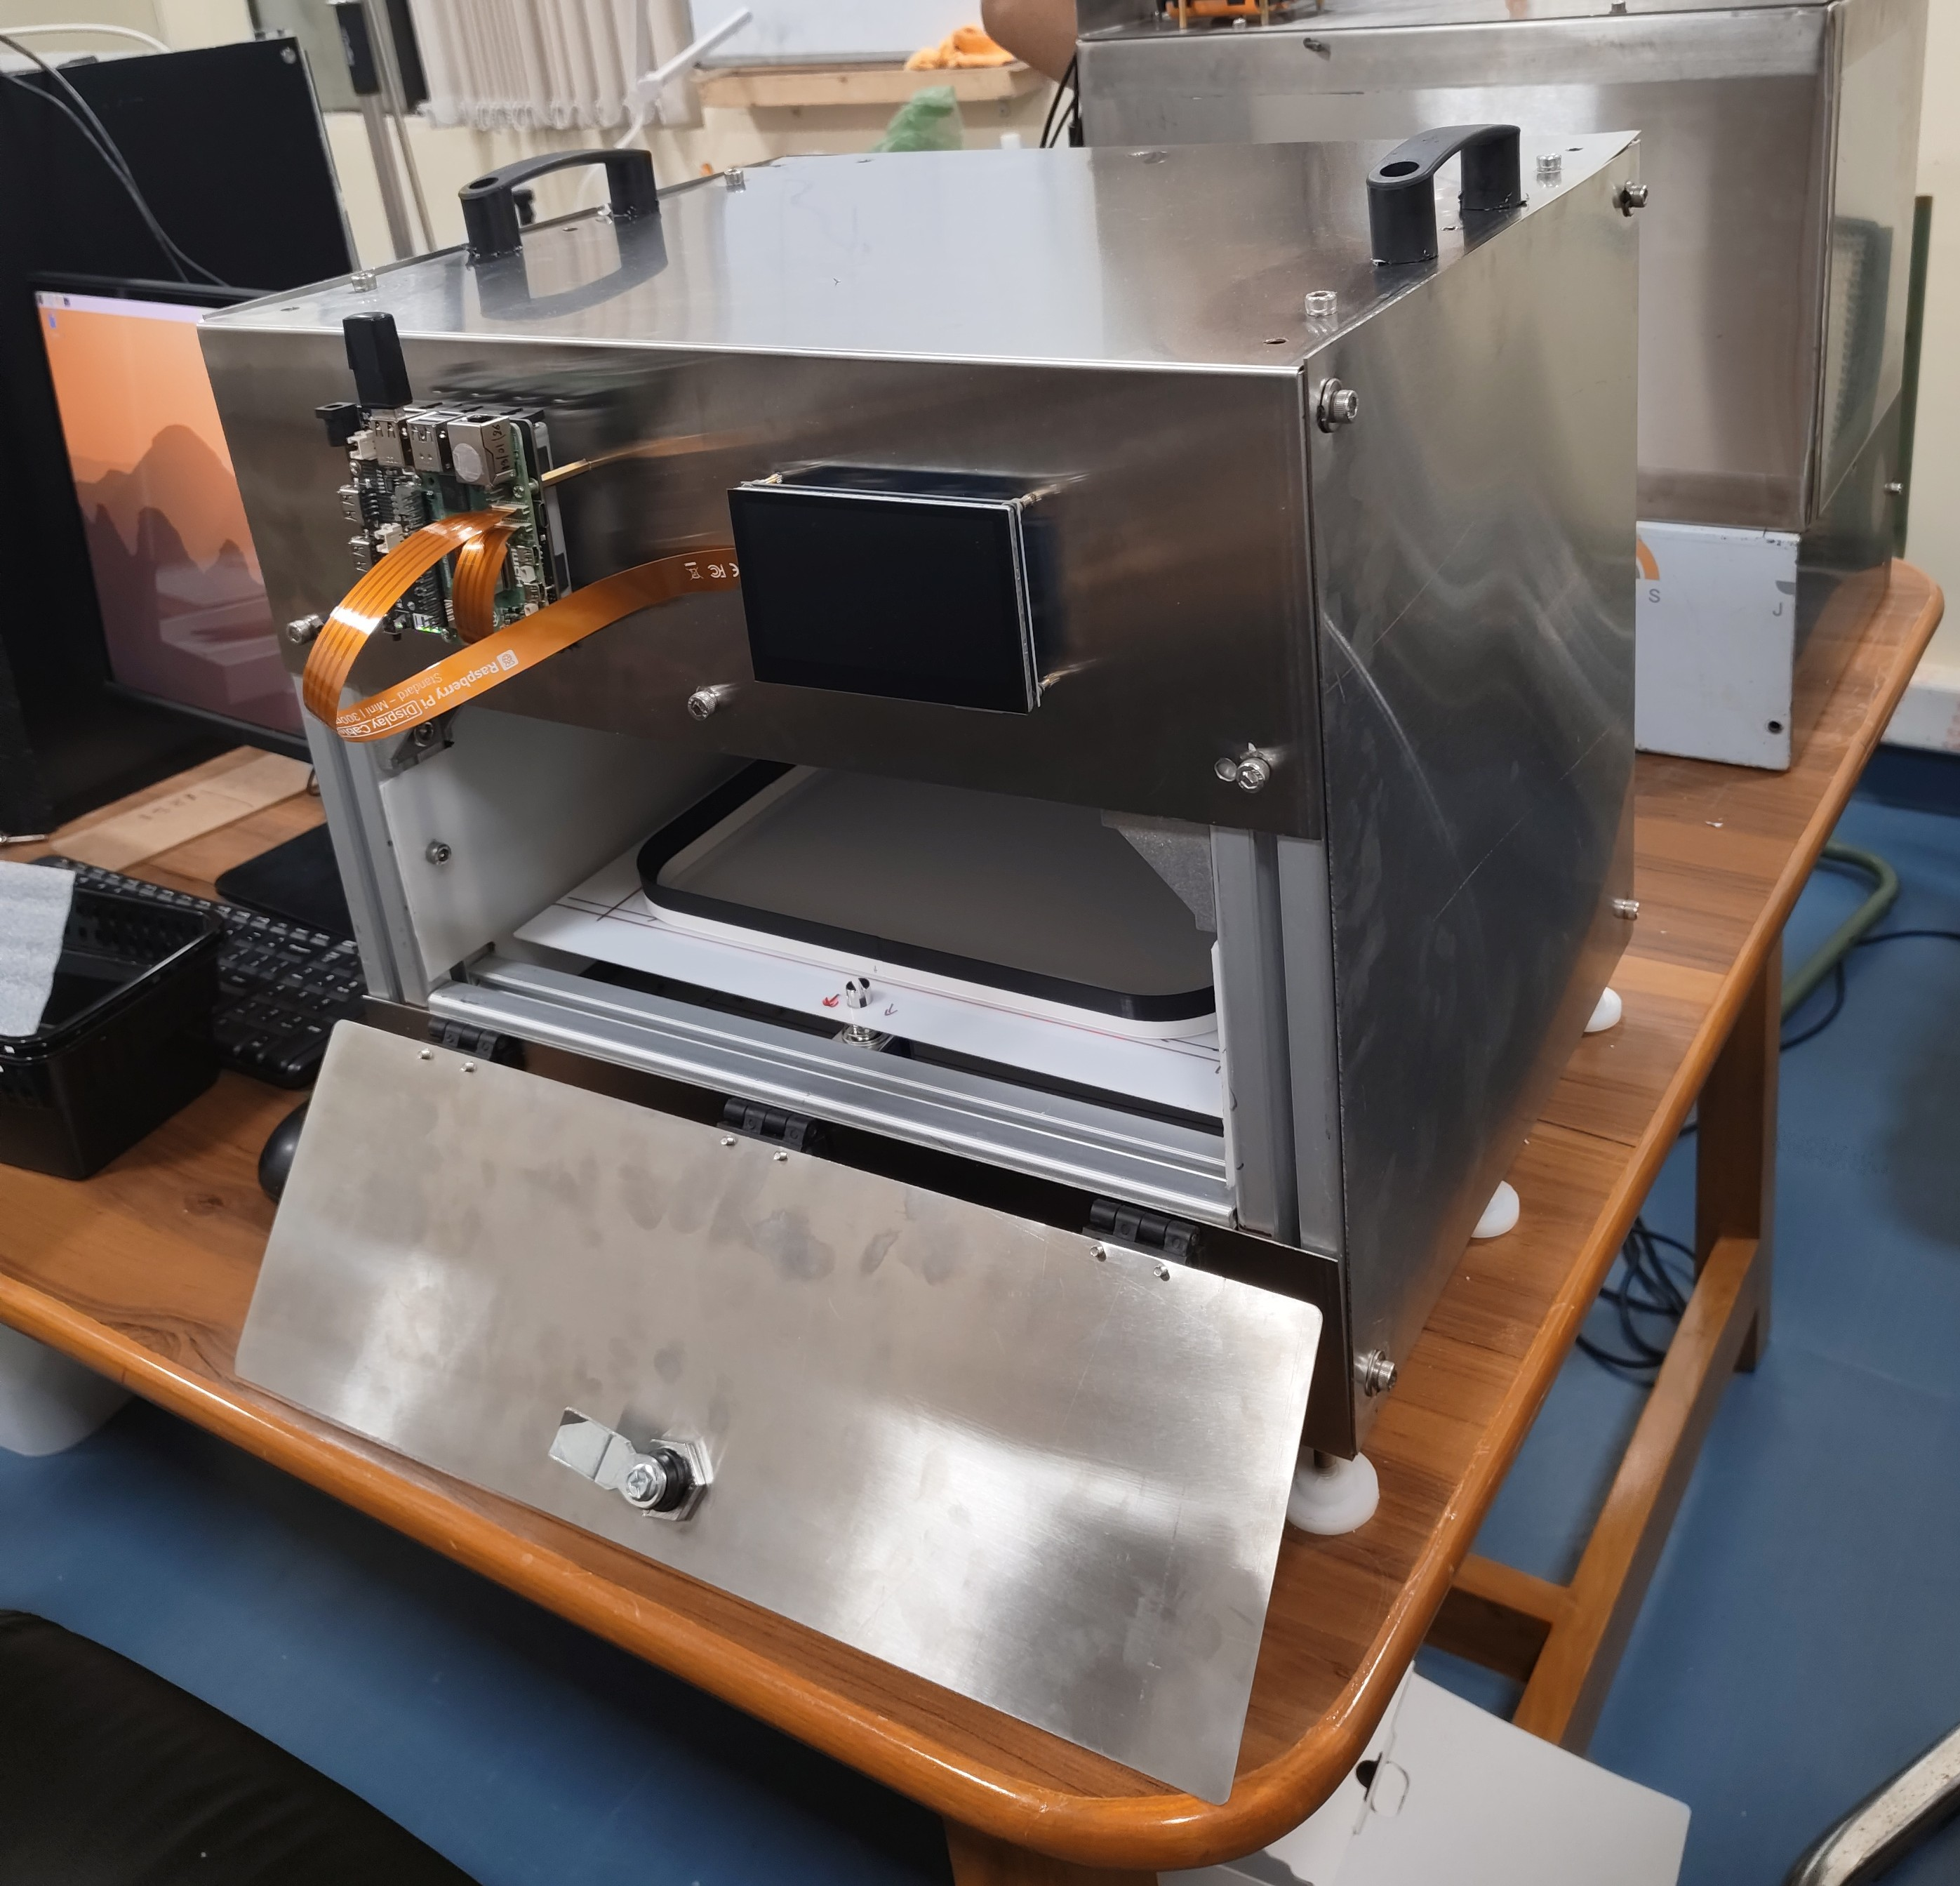
\includegraphics[width=0.6\textwidth]{final prototype photo.jpg}
    \caption{The finalised Drishti device with the hole-fitting grain tray, positioned for sample loading.}
    \label{fig:figure7_1}
\end{figure}

%----------------------------------------------------------------------------------------
\section{The Digital Dashboard: Information Hierarchy in Practice}
%----------------------------------------------------------------------------------------

The dashboard design problem was specific: the device produces a classification across twelve categories, each with a $W/W\%$ value, each compared against a threshold, and each potentially relevant to the accept/reject decision. Presenting twelve numbers simultaneously to an operator under time pressure is not informative; it is overwhelming. Tufte's \cite{Tufte2001} principle of information hierarchy---that the most important information should be visually dominant---was applied directly.

The primary visual element on the results screen is the overall verdict: Accept or Reject, displayed in a large, colour-coded format that requires no interpretation. The secondary layer shows which categories are out-of-threshold, with visual indicators that communicate compliance relative to the limit rather than raw numbers that require mental arithmetic. The tertiary layer---detailed category-by-category breakdowns---is available for operators who want to understand why a result was reached, but it does not appear unless requested.

Three specific features were designed in direct response to observed workflow patterns from the contextual inquiry:

\textbf{One-Touch Testing:} The full assessment cycle launches from a single operator action after tray placement. No intermediate confirmations, no parameter adjustment, no form-filling mid-cycle. The observation from the field was that interruptions in a continuous flow task increase error rate; one-touch launch minimises the number of such interruptions.

\textbf{Threshold Visualisation:} Each category result is shown as a position relative to its acceptance threshold rather than as an isolated number. An operator does not need to remember that the \textit{Broken} limit is 2.5\% and compare it against the displayed value; the display does that comparison and shows the result directly.

\textbf{Admin Review for Near-Threshold Cases:} Any category result within $\pm 2\%$ of threshold triggers an Admin Review flag rather than automatic Accept/Reject finalisation. The reasoning behind this feature came directly from watching quality managers at the factory site: the decisions they found most difficult---and most consequential---were not clear passes or clear failures, but the borderline cases where the number was within the margin and the appropriate response depended on context that the number alone did not capture. Admin Review holds those cases for expert attention rather than resolving them automatically.

\begin{figure}[H]
    \centering
    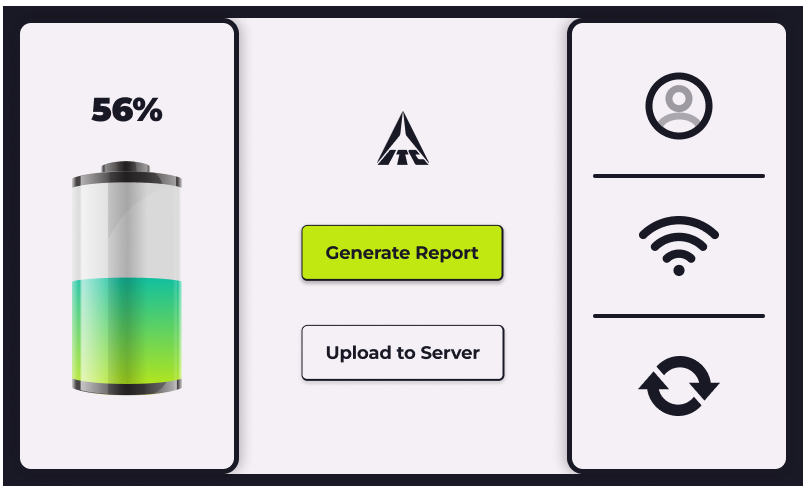
\includegraphics[width=0.75\textwidth]{GUI Home Screen.png}
    \caption{The Home Screen provides a clear, distraction-free starting point for the operator.}
    \label{fig:gui_home}
\end{figure}

The workflow begins at the \textbf{Home Screen} (Figure~\ref{fig:gui_home}), which is intentionally kept minimal to reduce cognitive load. A single tap launches the assessment, reducing the number of intermediate confirmations and preventing mid-cycle interruptions.

\begin{figure}[H]
    \centering
    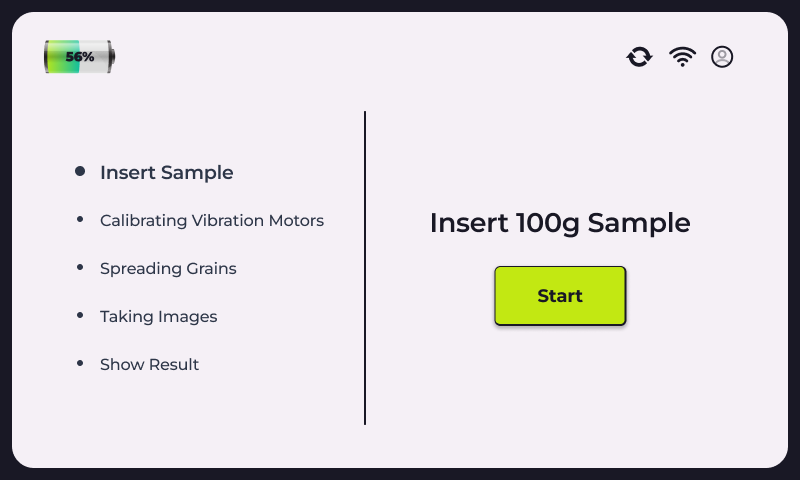
\includegraphics[width=0.75\textwidth]{GUI Step 1.png}
    \caption{Step 1: Sample Insertion prompt, ensuring the operator has correctly placed the tray before proceeding.}
    \label{fig:gui_step1}
\end{figure}

Following initiation, \textbf{Step 1} (Figure~\ref{fig:gui_step1}) explicitly prompts the operator to insert the loaded grain tray. This step guarantees that the physical interface is securely seated in the hole-fitting mechanism before any mechanical actuation begins.

\begin{figure}[H]
    \centering
    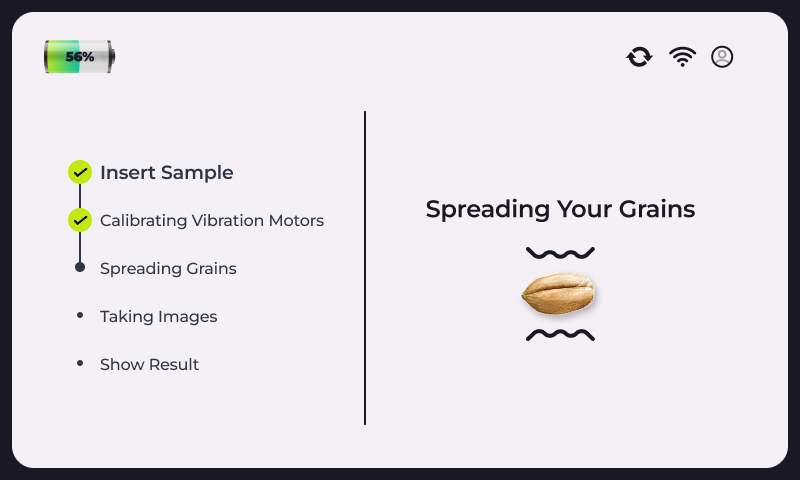
\includegraphics[width=0.75\textwidth]{GUIStep 3.png}
    \caption{Step 3: Real-time optoelectrical calibration feedback.}
    \label{fig:gui_step3}
\end{figure}

During \textbf{Step 3} (Figure~\ref{fig:gui_step3}), the system performs an optoelectrical calibration sequence. The interface displays real-time feedback, reassuring the operator that the system is actively adjusting to current ambient and internal lighting conditions.

\begin{figure}[H]
    \centering
    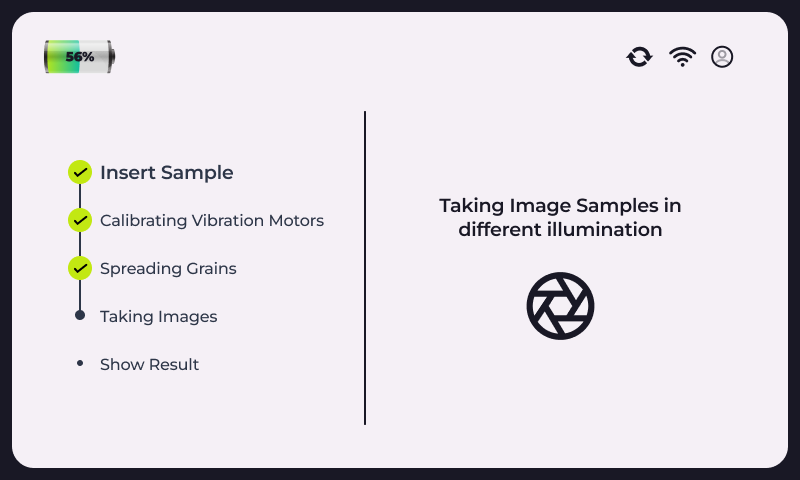
\includegraphics[width=0.75\textwidth]{GUI Step 4.png}
    \caption{Step 4: Image capture sequence, communicating progress as multiple frames are acquired.}
    \label{fig:gui_step4}
\end{figure}

\textbf{Step 4} (Figure~\ref{fig:gui_step4}) visualises the multi-frame capture process. As the solenoids induce granular dispersion, the progress indicator clearly shows the operator how many captures have been completed, setting clear expectations for the cycle duration without requiring manual intervention.

\begin{figure}[H]
    \centering
    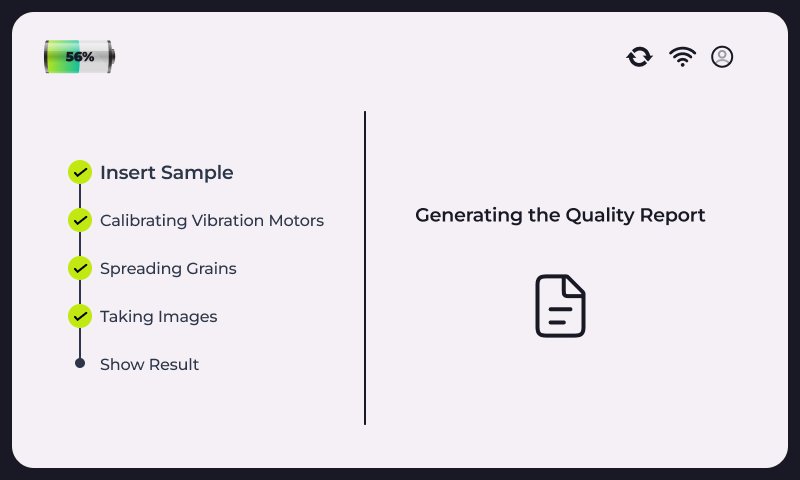
\includegraphics[width=0.75\textwidth]{GUI Step 5.png}
    \caption{Step 5: The final Quality Report, using threshold-relative visualisations for immediate interpretability.}
    \label{fig:gui_step5}
\end{figure}

Finally, \textbf{Step 5} (Figure~\ref{fig:gui_step5}) presents the comprehensive quality report. Instead of showing isolated numbers that require mental arithmetic, each category result is displayed relative to its specific acceptance threshold. The overall verdict (e.g., Accept, Reject, or Admin Review) is immediately visible at a glance, driving the final procurement decision.

%----------------------------------------------------------------------------------------
\section{Error Visibility and Graceful Degradation}
%----------------------------------------------------------------------------------------

A system that communicates its failure states as clearly as its success states is a safer system to rely on \cite{Shneiderman2016}. Three failure modes specific to the field deployment context were identified and addressed in the interface design.

\textbf{Grain overload detection:} If a tray is loaded with more than a standard 100-gram sample, or if grain distributes in a configuration that resists dispersion, segmentation density monitoring detects the anomalous state and prompts the operator to redistribute before proceeding. The alternative---silently generating an estimate from an inadequately dispersed sample---is worse than no estimate at all.

\textbf{Optical contamination alert:} Image quality metrics are monitored during the capture sequence. If dust accumulation on the imaging surface has degraded optical clarity to a level that could affect inference reliability, the dashboard flags a cleaning prompt and prevents new assessment submission until the operator confirms cleaning is complete.

\textbf{Connectivity status:} Because inference runs on a remote server, network state is always visible in the interface status bar. On connection loss, the system holds the captured frame sequence in a local queue and resubmits automatically when connectivity is restored, so that an assessment in progress is not simply abandoned.

%----------------------------------------------------------------------------------------
\section{Summary}
%----------------------------------------------------------------------------------------

The HDI design decisions in this chapter share a common origin: each of them came from watching the actual process fail, or from anticipating specific ways the automation could introduce new failure modes of its own. The drawer was replaced not because the hole-fitting mechanism was the theoretically superior design pattern, but because the drawer accumulated dust in a way that would have made it unusable within weeks. Admin Review was added not as a hedge against the system's limitations, but because observing quality managers made it clear that not all borderline decisions should be automated---some of them are genuinely judgment calls that require context only a human carries. The interface attempts, in each of these ways, to be honest about what the system can and cannot do dependably.

% Chapter 8 --- Results and Expert Validation

\chapter{Results and Expert Validation}\doublespacing
\label{Chapter8}
\lhead{Chapter VII. \emph{Results and Expert Validation}}

%----------------------------------------------------------------------------------------
\section{Introduction}
%----------------------------------------------------------------------------------------

% Note to author: This chapter should be completed following the conclusion of the
% June field trials at the five factory locations. The sections below provide the
% structural framework and describe the validation methodology conducted at the
% Bangalore headquarters demonstration. Quantitative accuracy figures, confusion
% matrices, and field trial performance data should be inserted once available.

It is worth being precise about what the validation conducted for this thesis did and did not establish. The research team visited wheat grain quality experts at ITC Limited's procurement warehouses and processing factories to evaluate the high-fidelity prototype against samples that experienced analysts consider particularly challenging. Food analysts and quality managers observed the device operating on real wheat samples and provided structured qualitative feedback. What this evaluation was not, and cannot be until multi-site field trials are completed, is a definitive performance benchmark. The distinction matters. The expert evaluation could assess whether the device behaved as intended and whether experienced evaluators judged its outputs to be plausible; it could not establish statistical confidence bounds on classification accuracy across the full range of seasonal and regional variation that characterises actual procurement conditions.

The validation was structured using heuristic evaluation principles \cite{Nielsen1994}, adapted to an industrial device context. Evaluators were asked to assess both the technical pipeline---whether dispersion, capture, and inference appeared to be working as described---and the operational interface, applying their own expertise to judge whether the system outputs matched their reading of the same grain samples.

A second, more rigorous validation phase across five factory sites is planned for completion following the June procurement season. The quantitative figures from that phase---per-category precision and recall, confusion matrices, and comparison against manual assessment baselines---will provide the evidentiary basis for claims about deployment readiness that the current chapter does not yet make.

%----------------------------------------------------------------------------------------
\section{Assessment Latency: Quantitative Comparison}
%----------------------------------------------------------------------------------------

The most immediately measurable improvement delivered by Drishti is the reduction in assessment cycle time. Manual assessment of a 100-gram wheat sample requires approximately 60 minutes per cycle. Drishti, deployed with a server-based inference backend, drastically reduces this duration depending on the inference hardware available.

\begin{figure}[H]
    \centering
    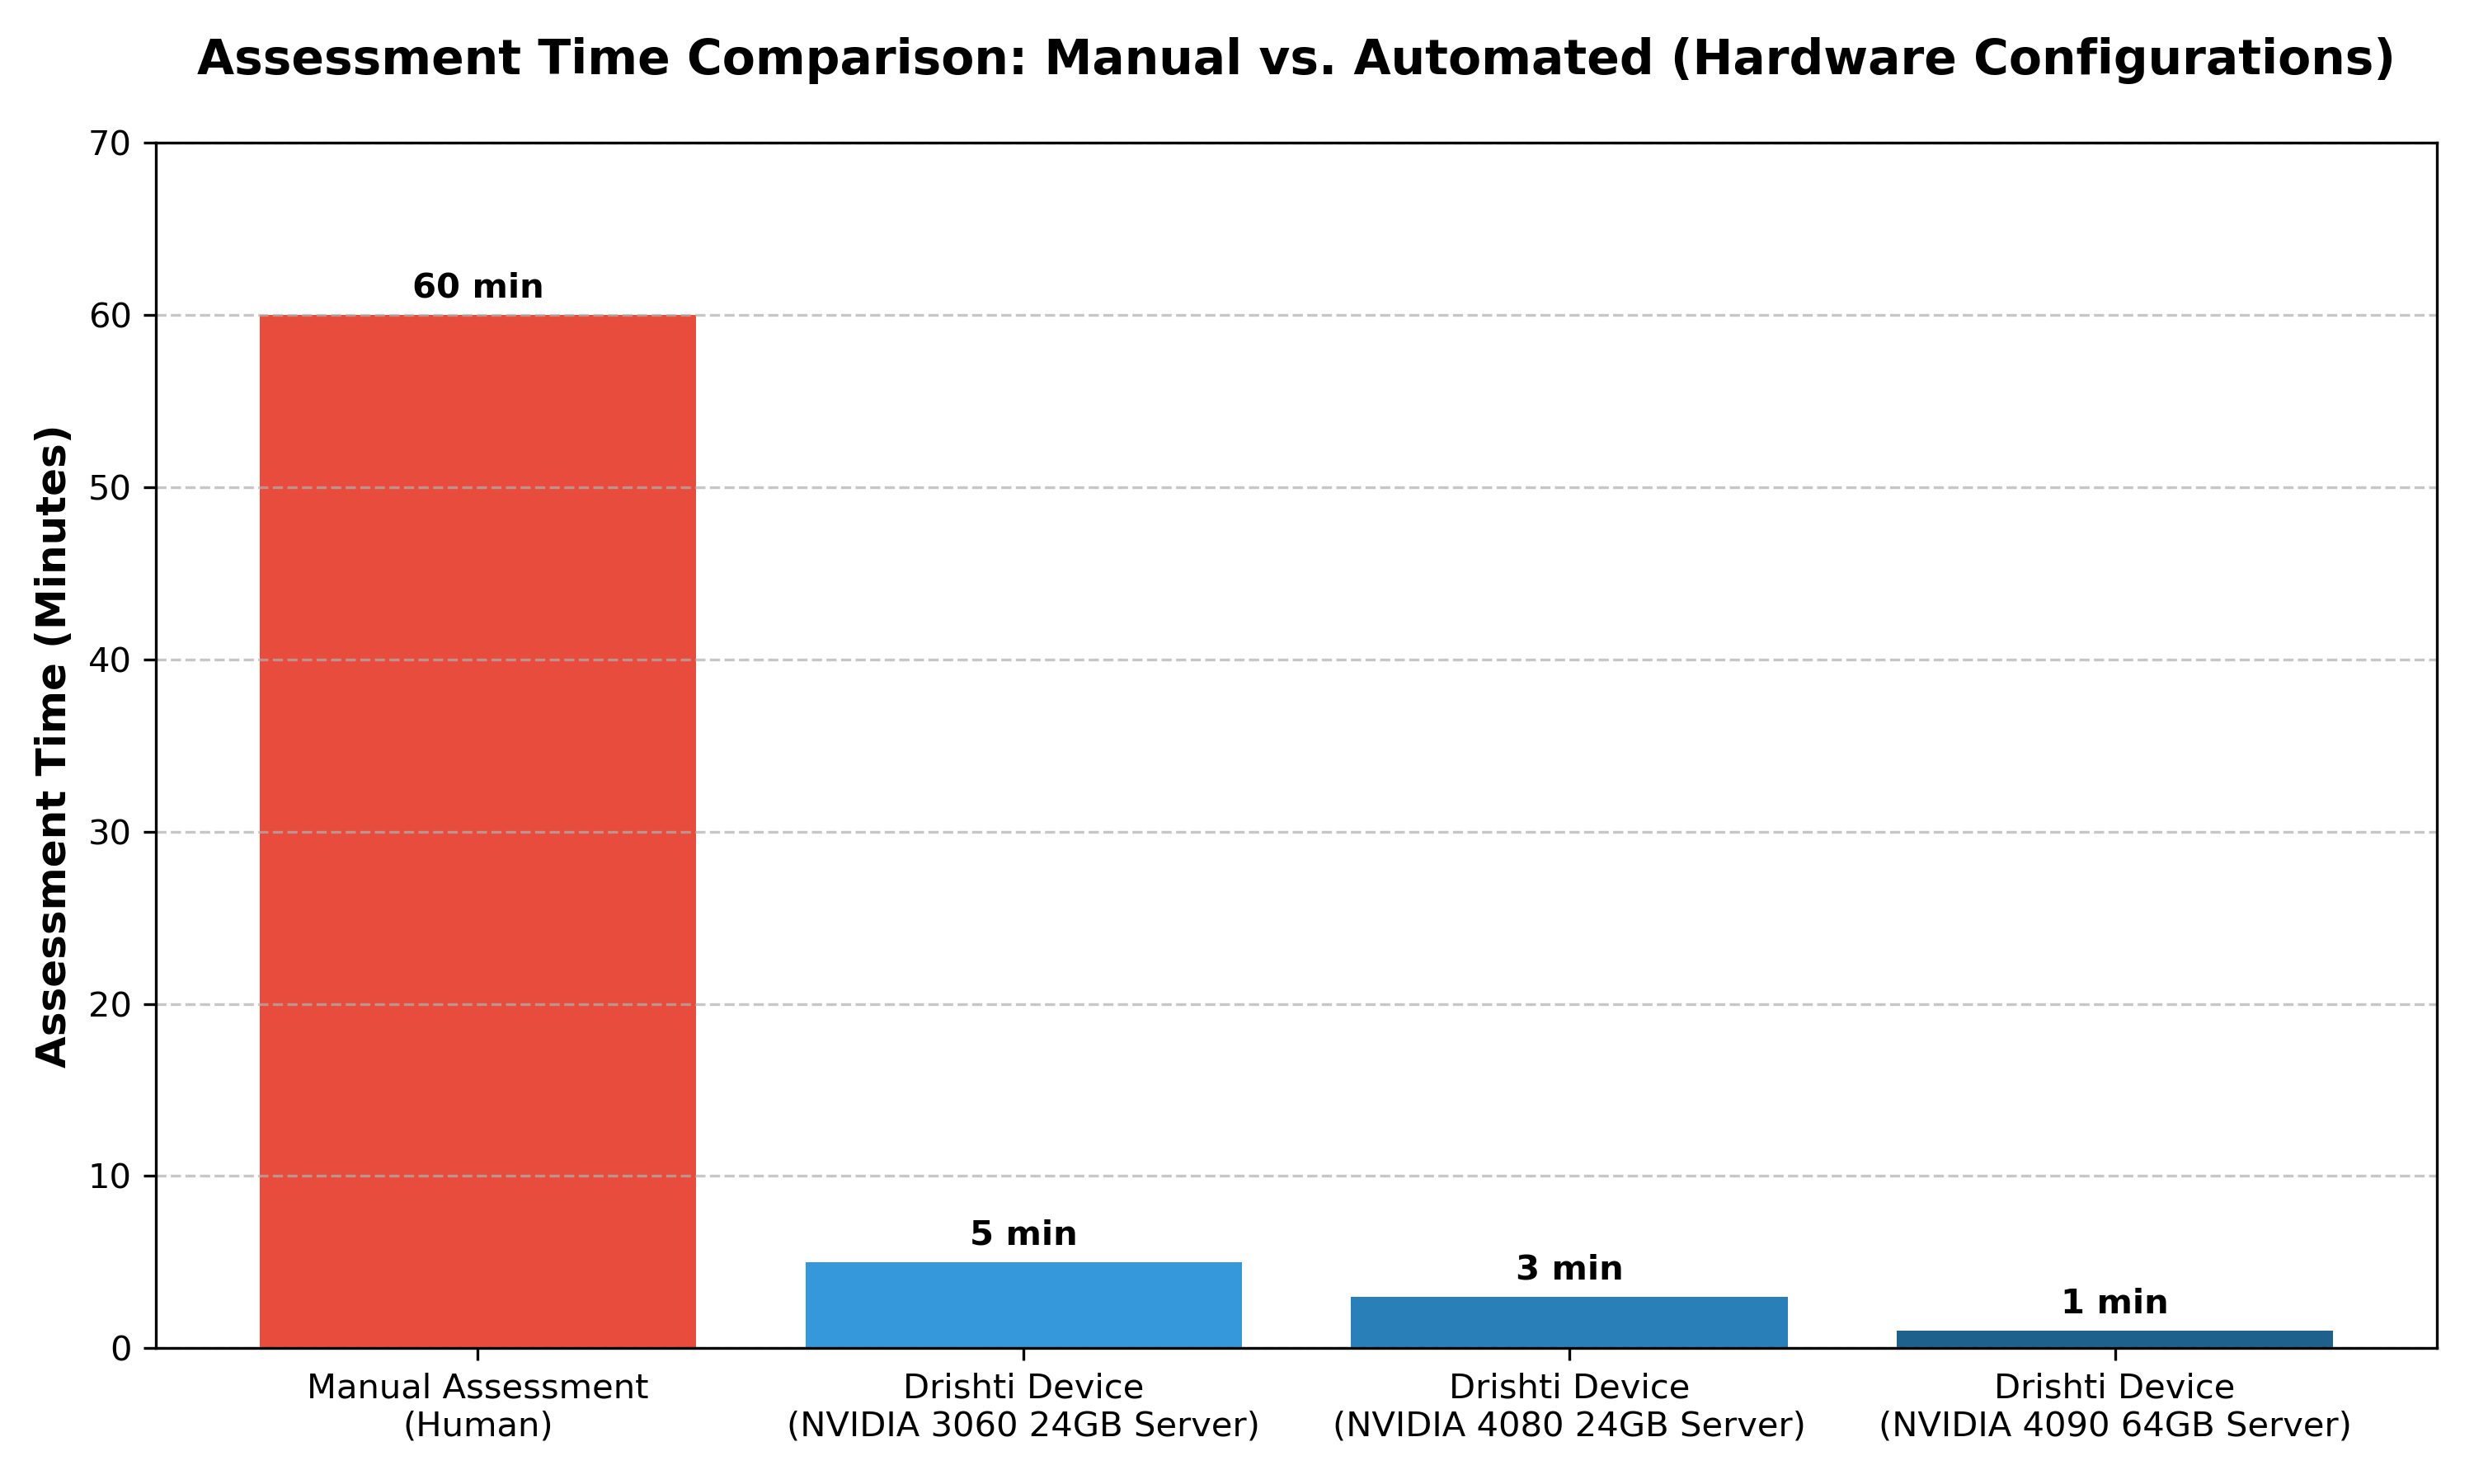
\includegraphics[width=0.95\textwidth]{Images/time_comparison.png}
    \caption{Comparison of assessment times between manual human inspection and the automated Drishti device across various GPU server configurations.}
    \label{fig:time_comparison}
\end{figure}

As illustrated in Figure~\ref{fig:time_comparison}, a baseline deployment using an NVIDIA RTX 3060 (24GB Server) completes the full assessment in approximately 5 minutes. Upgrading to an NVIDIA RTX 4080 (24GB Server) reduces this to 3 minutes, while a high-end NVIDIA RTX 4090 (64GB Server) can process the entire pipeline in just 1 minute. This acceleration represents a paradigm shift for high-volume procurement environments, allowing operations to scale without creating a bottleneck at the quality gate.

The reduction from 60 minutes to under 5 minutes is not merely a convenience improvement; it is a structural change in how procurement logistics can be organised. A shift that previously required a full hour per lot can be completed before the truck queue builds to the point where delays propagate through the supply chain.

%----------------------------------------------------------------------------------------
\section{Evaluation of the Mechanical Dispersion System}
%----------------------------------------------------------------------------------------

% Note to author: Insert quantitative dispersion metrics (coverage percentage
% across frames, mean entity isolation rate, spillage incident rate) when available.

The aspect of the prototype that generated the most immediate interest from evaluators was the solenoid dispersion mechanism. Analysts who had spent years sorting wheat grain manually were quick to identify that the staggered-impulse actuation was doing something that vibration-based systems typically do not: producing genuine grain rotation, not just lateral redistribution. This was noted specifically in the context of \textit{Infested} specimens, where the ventral-side entry marks that are one of the most reliable diagnostic features were described as becoming visible in the image sequence in a way that a static loading would not have supported.

The hole-fitting tray interface was operated by each evaluator without instruction beyond a brief demonstration. The drop-in placement motion, which had been a point of design uncertainty during development, was adopted quickly and generated no negative feedback. Evaluators noted that the absence of rails or latches was an improvement over their expectation---dust management was mentioned explicitly by one quality manager as a practical benefit.

No tray instability or spillage was observed across the demonstration cycles. Full quantitative coverage metrics---percentage of sample entities exposed across the frame sequence, mean isolation rate between actuation cycles---are deferred to the field trial phase.

%----------------------------------------------------------------------------------------
\section{Classification Performance}
%----------------------------------------------------------------------------------------

% Note to author: Insert confusion matrix, per-category precision/recall/F1 scores,
% and comparison against manual assessment baseline when available.

The domain-specific model was evaluated against parallel expert assessment on the same wheat lot samples used in the demonstration. The full statistical analysis is pending; the preliminary observations from Bangalore are recorded here as indicative findings, not final conclusions.

Major category detection---pure wheat, foreign matter including stone and chaff, and premium variety separation---produced outputs that evaluators assessed as consistent with their own manual readings of the same samples. The distinction between \textit{Sharbati} and \textit{Lokwan} specimens, which experienced assessors treat as reliable but junior assessors find difficult, was handled correctly in the cases reviewed during the demonstration.

Performance on orientation-sensitive defect categories was noted as appearing stronger than evaluators had expected from a single-camera system. The food analysts attributed this directly to the multi-frame capture approach, confirming the core hardware-software co-design hypothesis: mechanical exposure of previously occluded surfaces produced observable improvement in the system's ability to detect defects whose diagnostic features are not visible from a static top-down view.

The confusable pairs---\textit{Kernel Burnt} versus dark-variety \textit{Pure Wheat}, early \textit{Infested} versus \textit{Broken}---remain the areas of greatest uncertainty until full quantitative data are available.

\begin{figure}[H]
    \centering
    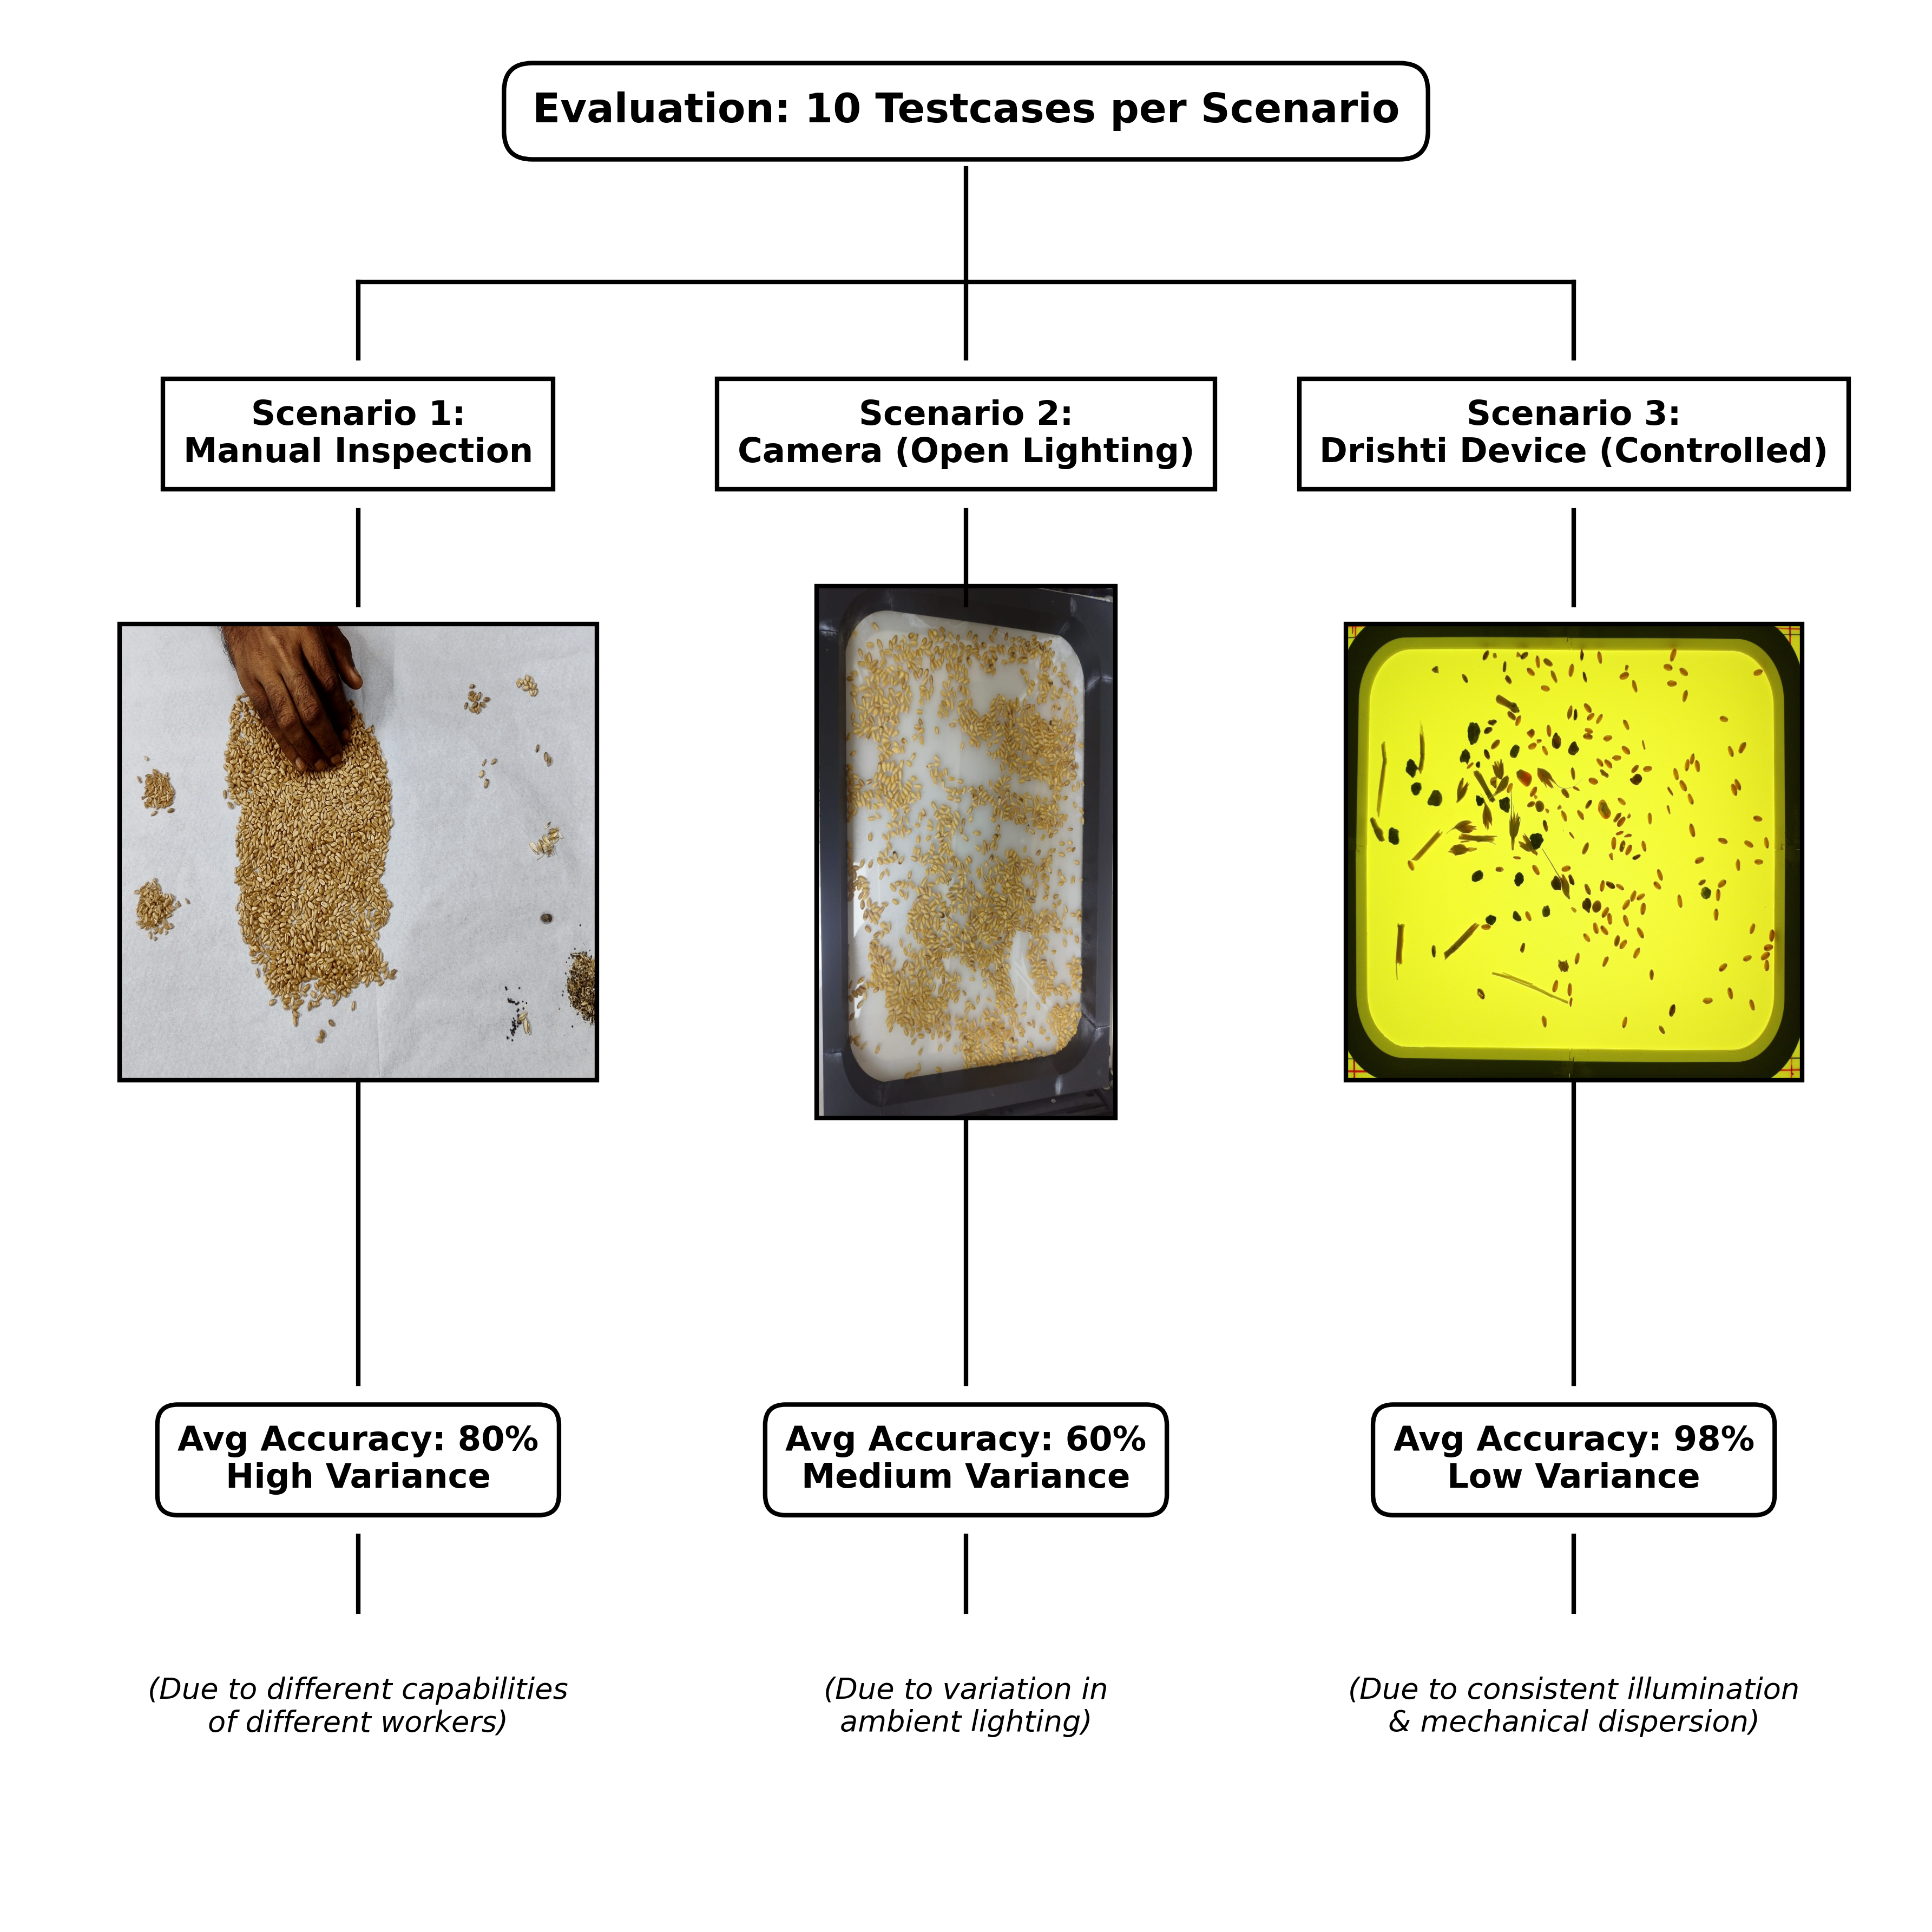
\includegraphics[width=0.95\textwidth]{Images/accuracy_flowchart.png}
    \caption{Comparative accuracy assessment across three inspection scenarios evaluated on ten standard test cases: manual inspection by an experienced technician, camera-based inspection in open uncontrolled lighting, and camera-based inspection within the Drishti device. The Drishti device's controlled illumination and multi-frame capture with solenoid dispersion consistently produced the highest accuracy across defect categories, particularly for orientation-sensitive cases such as Infested and Kernel Burnt grains.}
    \label{fig:accuracy_flowchart}
\end{figure}

%----------------------------------------------------------------------------------------
\section{Expert Feedback: Design and Interface Evaluation}
%----------------------------------------------------------------------------------------

The structured feedback session following the demonstration produced observations across both interaction layers.

On physical handling, the consensus was that tray operation was faster than evaluators had anticipated and that the full cycle sequence was comprehensible without explanation. One evaluator noted that having a device that could be loaded in the same time it takes to walk back to the sorting station was operationally meaningful---a comment that reflects exactly the kind of integration concern that emerged from the fieldwork.

On the digital interface, threshold visualisation was rated more immediately interpretable than the numerical tabular format used in existing warehouse assessment records. The distinction appeared most pronounced among senior managers, who described the threshold-relative indicators as making borderline cases more visible rather than requiring mental comparison of a number against a remembered limit. The Admin Review feature for $\pm 2\%$ threshold samples received explicit approval from senior quality managers, who framed it as consistent with how they already exercise oversight in manual assessment---reviewing borderline calls personally rather than delegating the finalisation of ambiguous results.

%----------------------------------------------------------------------------------------
\section{Summary}
%----------------------------------------------------------------------------------------

The Bangalore evaluation provided early and largely positive evidence for the two central claims of this thesis: that hardware-software co-design can address the physical observability constraints that limit single-image grain assessment, and that field-grounded interface design produces a device that operates meaningfully within the actual workflow rather than alongside it. What the evaluation does not provide, and what should not be claimed from it, is performance certainty across the conditions that matter most for deployment. That requires the multi-site field trials that follow. The Bangalore demonstration is a beginning, not a conclusion.

% Chapter 9 --- Conclusion and Future Work

\chapter{Conclusion and Future Work}\doublespacing
\label{Chapter9}
\lhead{Chapter IX. \emph{Conclusion and Future Work}}

%----------------------------------------------------------------------------------------
\section{Summary of Findings}
%----------------------------------------------------------------------------------------

The problem this thesis addressed was stated in operational terms at the outset: a quality assessment cycle that takes sixty minutes is a bottleneck. But the more important finding was not about speed. It was about the nature of the problem that made speed difficult to achieve without sacrificing accuracy---and why that problem had a design solution rather than simply an algorithmic one.

Dense grain samples do not cooperate with overhead cameras. They pile up, obscure each other, and present their surfaces in orientations that happen to hide the diagnostic features most relevant to the category calls that matter most. No model, however well-trained, can classify what it cannot see. This is not a gap in the current state of computer vision; it is a consequence of physics. The research contribution of Drishti is the recognition that the right response to this constraint is not to build a better model but to build a system that ensures the model is never asked to classify from hidden evidence.

Three specific findings support this claim. First, the high-density packing of a 100-gram sample---approximately 2,800 grain entities---creates occlusion that purely software-based approaches cannot reliably resolve, and any system that does not address this physically will produce estimates with an uncharacterisable bias in the direction of over-representing whatever happened to land on the surface. Second, staggered solenoid actuation ($T_A$ through $T_D$ at 50\,ms offsets) provides effective dispersion and orientation diversity across the image sequence; vibration, the more obvious alternative, does not, for reasons that took several experimental cycles to understand. Third, the hardware-software co-design approach---shaping the physical observability of the sample to support tractable inference---enabled a cycle time reduction compatible with operational requirements while producing outputs that ITC food analysts judged to be consistent with their own assessments of the same samples.

%----------------------------------------------------------------------------------------
\section{Contribution to Industrial Design Practice}
%----------------------------------------------------------------------------------------

This thesis is an Industrial Design thesis, not a machine learning thesis. The distinction is worth spelling out. The technical contributions---the solenoid timing logic, the calibration pipeline, the server-client deployment architecture---are important, but they are in service of a design argument. That argument is that the way a device structures the physical conditions of observation is as much an engineering decision as the algorithm running inside it, and that Industrial Design is a discipline with the right tools to make that decision well.

Two transferable design patterns emerge from this work for practitioners designing AI-integrated industrial devices.

The first is \textbf{Active Vision}: the deliberate engineering of physical conditions to improve the quality of visual information entering an inference system \cite{Aloimonos1988}. In Drishti, this means the solenoid actuation mechanism, the dual-illumination optics, the fixed white-balance calibration, and the frame-sequence capture strategy are not separate features---they are a single integrated strategy for giving the model a better problem to solve. This pattern is transferable to any inspection context where the natural presentation of the subject is unfavourable for the imaging geometry.

The second is \textbf{Human-Centred AI at decision interfaces}: the principle that automation should be applied to the part of a decision where it is most reliable, and human judgement should be preserved at the part where it is most valuable \cite{Shneiderman2020}. The Admin Review mechanism, which holds near-threshold results for expert consideration rather than resolving them automatically, is an expression of this. It is not a hedge against the system's accuracy; it is an acknowledgement that some decisions carry enough consequence that the confidence threshold for automated resolution should be higher than for routine clearances.

%----------------------------------------------------------------------------------------
\section{Limitations and Future Work}
%----------------------------------------------------------------------------------------

The limitations of this research are specific enough to be stated plainly rather than in the conventional register of academic hedging.

The Bangalore validation was an expert demonstration, not a longitudinal deployment. It could establish that the device worked as intended and that experienced evaluators found its outputs plausible; it could not establish how the system performs across the seasonal and regional variation in wheat quality, variety mix, and supply-chain handling practices that characterises ITC's network over a full procurement season. That validation requires the multi-site field trials scheduled for completion after the time of writing.

The training dataset, while domain-specific and acquisition-matched to the device, was finite in defect diversity. Edge-case defect presentations---unusual adulteration patterns, damage signatures from atypical handling conditions, morphologies from wheat varieties not yet represented in training---may produce lower-confidence or incorrect classifications. Understanding the distribution of such failures is only possible at scale.

Three directions for future work are identified as most productive:

\textbf{Large-scale field validation:} Complete multi-site trials and use the resulting error distribution to identify the specific failure modes that warrant targeted model refinement. The goal is not simply to improve aggregate accuracy but to understand where the system fails and whether those failures are systematic or random.

\textbf{Extension to adjacent commodities:} The hardware-software co-design framework developed for wheat is not wheat-specific. Rice, pulses, coffee beans, and spices all involve dense-entity inspection problems with orientation-sensitive quality attributes. The platform's mechanical and optical architecture could be adapted to these domains with commodity-specific dataset development and threshold calibration.

\textbf{Predictive quality analytics:} Sustained deployment at multiple sites will generate a longitudinal record of quality assessment results that has value beyond individual accept/reject decisions. Patterns across vendors, seasons, and storage conditions visible in that record could support predictive models of procurement risk that would be informative at a supply chain planning level rather than only at the point of intake.

%----------------------------------------------------------------------------------------
\section{Closing Reflection}
%----------------------------------------------------------------------------------------

The most experienced wheat assessors at ITC's procurement sites are doing something genuinely impressive: reading subtle morphological cues from thousands of grain entities under time pressure, in difficult conditions, and producing judgements that hold up against subsequent chemical analysis. That expertise took years to develop and exists in a small number of people. It is not robust to shift length, to staff turnover, or to the simple fact that the procurement season is finite and the demand for consistent quality assessment is not.

Drishti was not designed to replace that expertise. It was designed to make consistent, reliable quality assessment available at more points, more reliably, than human expertise alone can sustain. The question of whether it succeeds at that---whether the results produced by the device are trustworthy enough to underpin procurement decisions across a full operating season---is a question that the field trials will answer. What the work in this thesis established is that the design direction is viable, and that the specific constraints of the problem point toward a class of solution that has not previously been applied to this context. That is, at least, a beginning.


\clearpage 

%----------------------------------------------------------------------------------------
%	APPENDICES
%----------------------------------------------------------------------------------------

\addtocontents{toc}{\vspace{2em}} 

\appendix 

% Appendix A — Wheat Quality Thresholds and Classification Categories

\chapter{Wheat Quality Thresholds and Classification Categories}

\label{AppendixA}

\lhead{Appendix A. \emph{Grain Classification Thresholds}}

This appendix documents the twelve grain and impurity categories central to standard wheat quality assessment protocols, and the corresponding $W/W\%$ thresholds against which each sample is evaluated. These thresholds were sourced from food analysts during the contextual inquiry phase and form the benchmark against which the Drishti classifier is calibrated.

\vspace{1em}

\begin{table}[h!]
\centering
\caption{Wheat grain classification categories and indicative $W/W\%$ thresholds as applied in procurement protocols. Specific threshold values are proprietary and represented here in generalised form.}
\label{tab:thresholds}
\begin{tabular}{llp{5cm}}
\toprule
\textbf{Category} & \textbf{Type} & \textbf{Notes} \\
\midrule
Pure Wheat          & Desired Output    & No upper threshold; higher $\%$ indicates quality. \\
Broken Wheat        & Affected Grain    & $W/W\%$ must remain below threshold. \\
Kernel Burnt        & Affected Grain    & Scorched pericarp; often ventral-side defect. \\
Infested            & Affected Grain    & Insect-bored or contaminated; ventral-side signature. \\
Black Tip           & Affected Grain    & Discolouration at embryo end; subtle chromatic marker. \\
Potia               & Affected Grain    & Immature or shrivelled kernel. \\
Shrunken            & Affected Grain    & Undersized due to growth conditions. \\
Sprouted            & Affected Grain    & Germination initiated; structural compromise. \\
Stone               & Impurity          & High density; settles during vibration. \\
Earth Balls         & Impurity          & Clumped soil; density-variable. \\
Chaff               & Impurity          & Low density; surface-presenting under vibration. \\
Other Impurities    & Impurity          & Miscellaneous non-wheat material. \\
\bottomrule
\end{tabular}
\end{table}

\vspace{1em}

The twelve-category framework above illustrates the classification complexity that the Drishti system is designed to replicate. The concentration of defects with ventral-side signatures (Kernel Burnt, Infested, Black Tip) directly motivated the development of the electromagnetic solenoid grain dispersion system documented in Chapter~\ref{Chapter5}.

% Appendix B — Solenoid Timing and GPIO Configuration

\chapter{Solenoid Actuation Parameters and GPIO Configuration}

\label{AppendixB}

\lhead{Appendix B. \emph{Solenoid Parameters}}

This appendix documents the hardware configuration parameters for the electromagnetic solenoid actuation system. These values represent the empirically determined optima identified through the iterative testing programme described in Chapter~\ref{Chapter5}.

\vspace{1em}

\begin{table}[h!]
\centering
\caption{Solenoid actuation parameters for the staggered pulse activation sequence.}
\label{tab:solenoid_params}
\begin{tabular}{lll}
\toprule
\textbf{Parameter} & \textbf{Value} & \textbf{Notes} \\
\midrule
Number of solenoids           & 4              & Mounted at cardinal midpoints of grain plate. \\
Inter-solenoid delay ($\Delta t$) & 50 ms      & Empirical optimum for shearing effect. \\
Activation duration per solenoid  & 500 ms     & Measured from individual trigger point. \\
Full cycle duration           & 650 ms         & From $T_A$ trigger to $T_D$ deactivation. \\
Cycles per inspection         & Variable       & Image capture interleaved between cycles. \\
GPIO library                  & RPi.GPIO       & Raspberry Pi 5, Python implementation. \\
\bottomrule
\end{tabular}
\end{table}

\vspace{1em}

\noindent The staggered activation sequence follows the timing model defined in Chapter~\ref{Chapter5}:

\begin{align}
    T_A &= t \nonumber \\
    T_B &= t + 50\,\text{ms} \nonumber \\
    T_C &= t + 100\,\text{ms} \nonumber \\
    T_D &= t + 150\,\text{ms} \nonumber
\end{align}

\vspace{1em}

\begin{table}[h!]
\centering
\caption{Camera and illumination parameters (static configuration, AWB disabled).}
\label{tab:camera_params}
\begin{tabular}{lll}
\toprule
\textbf{Parameter} & \textbf{Value} & \textbf{Notes} \\
\midrule
Camera module         & Raspberry Pi HQ Camera   & 12.3 MP Sony IMX477 sensor. \\
Lens                  & 16mm telephoto            & Chosen for working distance to grain plane. \\
Shutter speed         & [To be specified]         & Set to eliminate motion blur during actuation. \\
White balance         & Fixed matrix (manual)     & Calibrated against colour reference chart. \\
Top illumination      & WS2812B RGB LED array     & Addressable; intensity tuned per variant. \\
Bottom illumination   & LCD backlight (dynamic)   & Colour programmable per wheat category. \\
Lux level (surface)  & [To be specified]         & Tuned to minimise specular highlights. \\
\bottomrule
\end{tabular}
\end{table}

\vspace{1em}
\noindent Parameters marked ``[To be specified]'' are to be completed following the finalisation of the imaging calibration protocol at ITC field sites.


\addtocontents{toc}{\vspace{2em}} 

\backmatter

%----------------------------------------------------------------------------------------
%	BIBLIOGRAPHY
%----------------------------------------------------------------------------------------

\label{References}

\lhead{\emph{References}} 
\renewcommand\bibname{References}
\bibliographystyle{unsrtnat} 

\bibliography{references} 

%\newpage
%\include{LOP}
% \newpage
% \chapter*{Biography}
\thispagestyle{plain}
\lhead{\emph{Biography}}

\noindent \textbf{[Your Name]} is a Master of Design candidate at the Indian Institute of Technology Kanpur, with a research focus on the intersection of industrial design, computer vision, and human-device interaction in agricultural FMCG supply chains.

\vspace{1em}

\noindent Prior to joining IIT Kanpur, [Your Name] completed their undergraduate studies in [Your Undergraduate Discipline] at [Your Undergraduate Institution]. The ``Drishti'' Wheat Grain Analyser, documented in this thesis, was developed in collaboration with ITC Limited as part of a sponsored research engagement with the Department of [Your Department].

\vspace{1em}

\noindent \textbf{Contact:} [your.email@iitk.ac.in]


\end{document}